% Self contained manuscript. Elsevier CAS support retains its original licence.
% Figures are supplied in the accompanying figures directory; bibliography is inline.
\begin{filecontents*}{cas-sc.cls}
%%
%% This is file `cas-dc.cls'.
%%
%% This file is part of the 'CAS Bundle'.
%% ......................................
%% 
%% It may be distributed under the conditions of the LaTeX Project Public
%% License, either version 1.3c of this license or (at your option) any
%% later version.  The latest version of this license is in
%%    http://www.latex-project.org/lppl.txt
%% and version 1.3c or later is part of all distributions of LaTeX
%% version 1999/12/01 or later.
%% 
%% The list of all files belonging to the 'CAS Bundle' is
%% given in the file `manifest.txt'.
%% 

%% $Id: cas-sc.cls 96 2024-05-04 09:29:44Z rishi $

 \def\RCSfile{cas-sc}%
 \def\RCSversion{2.4}%
 \def\RCSdate{2024/05/04}%
\NeedsTeXFormat{LaTeX2e}[1995/12/01]
\ProvidesClass{\RCSfile}[\RCSdate, \RCSversion: Formatting class
   for CAS single column articles]
%
\def\ABD{\AtBeginDocument}
%
% switches
% 
\newif\iflongmktitle    \longmktitlefalse
\newif\ifdc             \global\dcfalse
\newif\ifsc             \global\sctrue
\newif\ifcasreviewlayout  \global\casreviewlayoutfalse
\newif\ifcasfinallayout   \global\casfinallayoutfalse

\newcounter{blind}
\setcounter{blind}{0}

\def\blstr#1{\gdef\@blstr{#1}}
\def\@blstr{1}
\newdimen\@bls
\@bls=\baselineskip

\DeclareOption{singleblind}{\setcounter{blind}{1}}
\DeclareOption{doubleblind}{\setcounter{blind}{2}}
\DeclareOption{longmktitle}{\global\longmktitletrue}
\DeclareOption{final}{\global\casfinallayouttrue}
\DeclareOption{review}{\global\casreviewlayouttrue}

\ExecuteOptions{a4paper,10pt,oneside,fleqn}
\DeclareOption*{\PassOptionsToClass{\CurrentOption}{article}}
\ProcessOptions
\LoadClass{article}

\RequirePackage{graphicx}
\RequirePackage{amsmath,amsfonts,amssymb}
\allowdisplaybreaks

\RequirePackage{expl3,xparse}
\@ifundefined{regex_match:nnTF}{\RequirePackage{l3regex}}{}
\RequirePackage{etoolbox}
\RequirePackage{booktabs,makecell,multirow,array,colortbl,dcolumn,stfloats}
\RequirePackage{xspace,xstring,footmisc}
\RequirePackage[svgnames,dvipsnames]{xcolor}

\ifbool{casreviewlayout}{\RequirePackage{setspace}}{}

\RequirePackage[colorlinks]{hyperref}
\colorlet{scolor}{black}
\colorlet{hscolor}{DarkSlateGrey}
\hypersetup{%
  pdfcreator={LaTeX3; cas-sc.cls; hyperref.sty},
  pdfproducer={pdfTeX;},
  linkcolor={hscolor},
  urlcolor={hscolor},
  citecolor={hscolor},
  filecolor={hscolor},
  menucolor={hscolor},
}
% \AtEndDocument{\hypersetup
%   {pdftitle={\csuse{__short_title:}},
%   pdfauthor={\csuse{__short_authors:}}}}
 
 \let\comma\@empty
\let\tnotesep\@empty
\let\@title\@empty
%
% Load Common items
%

\RequirePackage{cas-common}

%
% Specific to Single Column
%
\ExplSyntaxOn

\RenewDocumentCommand \maketitle {}
{
  \ifbool { usecasgrabsbox }
    { 
      \setcounter{page}{0}
      \thispagestyle{empty}
      \unvbox\casgrabsbox  
    } { }  
  \pagebreak  
  \ifbool { usecashlsbox }
    { 
      \setcounter{page}{0}
      \thispagestyle{empty}
      \unvbox\casauhlbox
    } { }    
  \pagebreak  
  \thispagestyle{first}
  \ifbool{longmktitle}
  {
    \ifnum\theblind>0\relax
        \LongMaketitleBox[blind]
    \else
		\LongMaketitleBox
    \fi
    \ProcessLongTitleBox
  }
  {
    \ifnum\theblind>0\relax
        \MaketitleBox[blind]
    \else
		\MaketitleBox
    \fi
    \printFirstPageNotes
  }
  \normalcolor \normalfont
  \setcounter{footnote}{\int_use:N \g_stm_fnote_int}
  \renewcommand\thefootnote{\arabic{footnote}}
  \gdef\@pdfauthor{\infoauthors}
  \gdef\@pdfsubject{Complex ~STM ~Content}
  \ifbool{casreviewlayout}{\doublespacing}{}
}

%
% Fonts
%
\RequirePackage[T1]{fontenc}

\file_if_exist:nTF { stix.sty }
{
  \file_if_exist:nTF { charis.sty }
  {
    \RequirePackage[notext]{stix} 
    \RequirePackage{charis}
  }
  { \RequirePackage{stix} }
}
{
  \iow_term:x {  *********************************************************** }
  \iow_term:x { ~Stix ~ and ~ Charis~ fonts ~ are ~ not ~ available ~ }
  \iow_term:x { ~ in ~TeX~system.~Hence~CMR~ fonts~ are ~ used. }
  \iow_term:x {  *********************************************************** }
}

\file_if_exist:nTF { inconsolata }
{ \RequirePackage[scaled=.85]{inconsolata} }
{ \tex_gdef:D \ttdefault { cmtt } }

\ExplSyntaxOff

%
% Page geometry
%

\usepackage[%
  paperwidth=192mm,
  paperheight=262mm,
%  vmargin={12.4mm,11.5mm},
  vmargin={19mm,19mm},
  hmargin={13.7mm,13.7mm},
  headsep=12pt,
  footskip=12pt,
]{geometry}


\endinput
  
%
% End of class 'cas-sc'
%


\end{filecontents*}
\begin{filecontents*}{cas-common.sty}
%%
%% This is file `cas-common.sty',
%%
%% This file is part of the 'CAS Bundle'.
%% ......................................
%% 
%% It may be distributed under the conditions of the LaTeX Project Public
%% License, either version 1.3c of this license or (at your option) any
%% later version.  The latest version of this license is in
%%    http://www.latex-project.org/lppl.txt
%% and version 1.3c or later is part of all distributions of LaTeX
%% version 1999/12/01 or later.
%% 
%% The list of all files belonging to the 'CAS Bundle' is
%% given in the file `manifest.txt'.
%% 

% $Id: cas-common.sty 94 2024-05-04 09:27:09Z rishi $

 \def\RCSfile{cas-common}%
 \def\RCSversion{2.4}%
 \def\RCSdate{2024/05/04}%
\NeedsTeXFormat{LaTeX2e}[1995/12/01]

\pretolerance=-1
\tolerance=1000
\hyphenpenalty=1000
\exhyphenpenalty=100
\brokenpenalty=10000
\vfuzz=\z@
\hfuzz=.2pt
\doublehyphendemerits=100
\emergencystretch=2pt
\frenchspacing
\clubpenalty=10000
\widowpenalty=10000

\ExplSyntaxOn
\makeatletter
%
% Front matter macros
%
% The front matter macros are derived/adopted from stm-prelims.sty
% written by CV Radhakrishnan <cvr@cvr.cc> and copyrighted by him.
% Usage of those macros and methods are gratefully acknowledged.
% 

\tl_set:Nn \l_stm_title_color_tl { black }

\keys_define:nn { stm / title }
   {
     mode      .choice:     ,
     mode / title  .meta:n  = 
       {
         type   = title      ,
         size   = \LARGE      ,
         shape  = \upshape   ,
         weight = \mdseries  ,
         color  = black  ,
         before = 0pt        ,
         after  = 0pt        ,
         align  = \raggedright ,
       } ,
     mode / alt  .meta:n  = 
       {
         type   = alt      ,
         size   = \large     ,
         shape  = \upshape   ,
         weight = \mdseries  ,
         color  = black  ,
         before = 6pt        ,
         after  = 0pt        ,
         align  = \raggedright ,
       } ,
     mode / sub    .meta:n  = 
       {
         type   = sub           ,
         size   = \large        ,
         shape  = \upshape      ,
         weight = \mdseries     ,
         color  = black!80  ,
         before = 6pt          ,
         after  = 0pt           ,
         align  = \raggedright  ,
       } ,
     mode / trans   .meta:n  = 
       {
         type   = trans         ,
         size   = \normalsize   ,
         shape  = \upshape      ,
         weight = \mdseries     ,
         color  = black!60      ,
         before = 6pt           ,
         after  = 0pt           ,
         align  = \raggedright  ,
       } ,
     mode / transsub   .meta:n  = 
       {
         type   = transsub      ,
         size   = \small        ,
         shape  = \upshape      ,
         weight = \mdseries     ,
         color  = black!50      ,
         before = 6pt           ,
         after  = 0pt           ,
         align  = \raggedright  ,
       } ,
     mode / ascii   .meta:n  = 
       {
         type   = ascii            ,
         size   = \small\ttfamily  ,
         shape  = \upshape         ,
         weight = \mdseries        ,
         color  = black            ,
         before = 12pt             ,
         after  = 0pt              ,
         align  = \raggedright     ,
       } ,
     type      .tl_set:N    = \l_stm_title_type_tl      ,  
     size      .tl_set:N    = \l_stm_title_size_tl      ,
     shape     .tl_set:N    = \l_stm_title_shape_tl     ,
     weight    .tl_set:N    = \l_stm_title_weight_tl    ,
     before    .dim_set:N   = \l_stm_title_before_dim   ,
     after     .dim_set:N   = \l_stm_title_after_dim    ,
     align     .tl_set:N    = \l_stm_title_align_tl     ,
     color     .tl_set:N    = \l_stm_title_color_tl     ,
   }

\NewDocumentCommand \processTmarks { }
   {
     \cs_if_free:cTF { mark@title }
     { \ignorespaces }
     { \tl_set:Nx \l_tmpa_tl { \cs:w mark@title\cs_end: }
       \clist_map_inline:cn { mark@title }
       {
         \str_case:nn { ##1 }
         {
           { 1 }  { $^\star$ } 
           { 2 }  { $^{,\star\star}$ }
           { 3 }  { $^{,\star\star\star}$ }
         } 
       }
     }
   }

\RenewDocumentCommand \title { O{} m }
   {
     \pdfstringdef \@pdftitle { #2 } 
     \csgdef { casprelimstitle } { #2 }
     \keys_set:nn { stm / title } { #1 }
     \seq_gput_right:Nn \g_stm_title_seq
      {
        \keys_set:nn { stm / title } { #1 }
%        \msg_term:n { MODE:~\l_stm_title_mode_tl ~ ~ [#2]}
        \par \vskip \l_stm_title_before_dim
        \l_stm_title_align_tl
        \l_stm_title_size_tl
        \l_stm_title_shape_tl
        \l_stm_title_weight_tl
        \color { \l_stm_title_color_tl }
        \noindent \unskip \ignorespaces #2
        \tl_set:Nn \l_tmpa_tl { title }
        \tl_if_eq:NNTF \l_stm_title_type_tl \l_tmpa_tl
        { \processTmarks } { }
        \par \vskip  \l_stm_title_after_dim 
        \normalcolor \normalsize \normalfont
      } 
     }

%  \gappto\usestmtitle{#1}%

\renewcommand \@title { \seq_use:Nn \g_stm_title_seq { } }

\NewDocumentCommand \wrAun { m }      %  unexpanded write to aux
   { \iow_now:Nn \@auxout { #1 } }
\NewDocumentCommand \wrAux { m }      %  expanded write to aux
   { \iow_now:Nx \@auxout { #1 } }

\NewDocumentCommand \wrShipAux { m }   % expanded write at shipout
   { \iow_shipout:Nx \@auxout { #1 } }
\NewDocumentCommand \wrShipAun { m }   % unexpanded write at shipout
   { \iow_shipout:Nn \@auxout { #1 } }

\NewDocumentCommand \stmLabel { m }
   {
     \@bsphack \wrAux
     { \token_to_str:N \NewLabel { #1 }
       { \@currentlabel }
     } \@esphack
   }
\NewDocumentCommand \NewLabel { m m }
   {
     \cs_if_free:cTF { X@#1: }
       { \cs_new:cx { X@#1: } { #2 } }
       { \cs_set:cx { X@#1: } { #2 } }
     }
\NewDocumentCommand \stmRef { m }
   {
    \cs_if_free:cTF { X@#1: }
      { 0 } {\use:c {X@#1:} } 
   }

\seq_clear_new:N \l_fnmk_seq
\NewDocumentCommand \processFnRef { m }
   {
      \seq_clear:N \l_fnmk_seq
      \clist_map_inline:nn { #1 }
      { \seq_put_right:Nx \l_fnmk_seq 
          {\cs_if_free:cTF { X@##1: } {0} { \use:c {X@##1:} }}
      }
    }

\NewDocumentCommand \fnmark { O{} }
   { \writemarks { fnau\theau@ } { #1 } }


\NewDocumentCommand  \fnref { m }
   {
     \processFnRef { #1 }
     \wrAux { \token_to_str:N \csxdef {mark@fnau\theau@}
         { \seq_use:Nn \l_fnmk_seq  { , } } }
   }

\NewDocumentCommand \corref { m }
   {
     \str_set:Nx \l_tmpa_str { \stmRef { #1 } }
     \wrAux { \token_to_str:N \csxdef { mark@corau\theau@ }
       {
         \cs_if_free:cTF { X@#1: } {0} { \use:c {X@#1:} }
       }
     }
   }

\NewDocumentCommand \cormark { O{} }
   {
     \@cormarktrue
     \writemarks {corau\theau@} { #1 } 
   }

\seq_new:N \l_stm_au_seq
\seq_new:N \l_stm_au_sn_seq
\seq_new:N \l_stm_au_fn_seq
\seq_new:N \l_stm_au_ead_seq
\seq_new:N \l_stm_au_orcid_seq
\seq_new:N \l_stm_au_contrib_role_seq

\NewDocumentCommand \parsename { m }
   { \seq_set_split:Nnn \l_stm_au_seq { ~ } {#1}
     \seq_pop_right:NN \l_stm_au_seq \l_stm_au_sn_seq
     \seq_map_inline:Nn \l_stm_au_seq
      { \seq_put_right:Nx \l_stm_au_ead_seq
        { \tl_head:n { #1 }. } } 
    }

\NewDocumentCommand \invparsename { m }
   { \seq_set_split:Nnn \l_stm_au_seq { ~ } {#1}
     \seq_pop_left:NN \l_stm_au_seq \l_stm_au_sn_seq
     \seq_map_inline:Nn \l_stm_au_seq
      { \seq_put_right:Nx \l_stm_au_ead_seq
        { \tl_head:n { #1 }. } } 
    }
     
    
\NewDocumentCommand \surname {} { \l_stm_au_sn_seq }
\NewDocumentCommand \firstname {} 
    { \seq_use:Nn \l_stm_au_seq { ~ } }
\NewDocumentCommand \eadauthor {} 
    { \seq_map_inline:Nn \l_stm_au_seq
      { \regex_match:nnTF { \. } { ##1 } 
        { ##1 }
        { \tl_head:n {##1}. }
      }
        {~} \l_stm_au_sn_seq
     }
\cs_set_eq:NN \shortauthor \eadauthor

\seq_clear_new:N \l_affmk_seq
\NewDocumentCommand \processAffRef { m }
   {
     \seq_clear:N \l_affmk_seq
     \clist_map_inline:nn { #1 }
     { 
       \seq_put_right:Nx \l_affmk_seq 
       {\stmRef{##1}}
      }
    }

\NewDocumentCommand \processAffNum { m }
   {
     \seq_clear:N \l_affmk_seq
     \clist_map_inline:nn { #1 }
     {
       \seq_put_right:Nn \l_affmk_seq 
       { \int_to_alph:n {##1} }
      }
    }

\NewDocumentCommand \listAff { }
   { 
     \tl_if_blank:nTF { \l_affmk_seq }
       { \tl_gset:Nn \g_stm_comma_tl { 0 } }
       {
         \seq_use:Nn \l_affmk_seq { , }
         \tex_def:D \sep{\unskip,}
       }
   }

\NewDocumentCommand \ead { O{} m }
   {
     \tl_if_empty:nTF { #1 } { \@ead {#2} } { \@uad[#1]{#2} } 
   }

\NewDocumentCommand \eadsep { } { }

\int_new:N \g_ead_int
\seq_new:N \g_stm_ead_seq
\int_new:N \g_uad_int
\seq_new:N \g_stm_uad_seq
\seq_new:N \g_stm_orcid_seq
\seq_new:N \g_stm_contrib_role_seq

\newcommand\theead { \int_use:N \g_ead_int }

\NewDocumentCommand \@uad { O{} m }
   {
     \group_begin:
     \wrAux { \token_to_str:N \urlauthor
       { \exp_not:n {#2}}{\the\@eadauthor}}%
     \group_end:
   }

\NewDocumentCommand \urlauthor { m m }
   {
     \int_gincr:N \g_uad_int
     \seq_gput_right:Nn \g_stm_uad_seq
       {
         { %\ttfamily \tl_to_str:n
           \url{ #1 } }
         \parsename { #2 }
         \space(\eadauthor)
       }
     }
\NewDocumentCommand \@stmuads { }
  { \seq_use:Nn \g_stm_uad_seq { ;~ } }

\NewDocumentCommand \@ead { m }
   {
     \group_begin:
     \wrAux { \token_to_str:N \emailauthor
       { \exp_not:n { #1 }}{ \the\@eadauthor }}
     \group_end:
   }

\newtoks \@eadauthor
\newbool{@cormark}

\NewDocumentCommand \emailauthor { m m }
   {
     \int_gincr:N \g_ead_int
     \seq_gput_right:Nn \g_stm_ead_seq
       {
         { \ttfamily \tl_to_str:n { #1 } }
         \parsename { #2 }
         \space(\eadauthor)%
       }
     }

\NewDocumentCommand \@elseads { }
  { \seq_use:Nn \g_stm_ead_seq { ;~ } }


\NewDocumentCommand \printemails { }
{
  \group_begin:
  \int_compare:nNnTF { \int_use:N \g_ead_int } > { 0 }
  {
    \tex_let:D \thefootnote \relax \footnotetext
    {
      \raggedright
      \bool_if:NTF \g_stm_nologo_bool
      { 
        \int_compare:nTF { \g_ead_int = 1 }
        { \textit{Email~address:\c_space_token} }
        { \textit{Email~addresses:\c_space_token} }
      }
      { \includegraphics[height=8pt]{thumbnails/cas-email.jpeg}\c_space_token } 
      \seq_use:Nn \g_stm_ead_seq { ;~ }
    }
  }
  {  }
  \group_end:
}

\NewDocumentCommand \printurls { }
{
  \group_begin:
  \int_compare:nTF { \g_uad_int > 0 }
  {
    \tex_let:D \thefootnote \relax \footnotetext
    {
      \raggedright
      \bool_if:NTF \g_stm_nologo_bool
      { \textit{URL:\c_space_token} } 
      { \includegraphics[height=8pt]{thumbnails/cas-url.jpeg}\c_space_token } 
      \seq_use:Nn \g_stm_uad_seq { ;~ }
    }
  }
  { }
  \group_end:
}

%
% orcid
%
\NewDocumentCommand \orcidauthor { m m }
   {
     \seq_gput_right:Nn \g_stm_orcid_seq
       {
         { \ttfamily \tl_to_str:n { #1 } }
         \parsename{#2}
         \space(\eadauthor)
       }
     }

\NewDocumentCommand \printorcid { }
{
  \group_begin:
    \tex_let:D \thefootnote \relax \footnotetext
    {
      \raggedright
      \textsc{orcid}(s):\c_space_token 
      \seq_use:Nn \g_stm_orcid_seq { ;~ }
    }
  \group_end:
}

%
% Contrib Role
%

\seq_gclear_new:N \g_stm_credits_seq

\NewDocumentCommand \ContribRole { m }
{
  \wrAux { \token_to_str:N \creditauthor
    { #1 } { \the\@eadauthor } }
}

\NewDocumentCommand \creditauthor { m m }
{
  \seq_gput_right:Nx \g_stm_credits_seq
  { { \exp_not:N\bfseries #2 :}\space #1 }
}

\cs_set_eq:NN \credit \ContribRole

\NewDocumentCommand \printcredits { }
{
  \seq_if_empty:NF \g_stm_credits_seq
  {
    \section*{CRediT ~authorship ~contribution ~statement}
    \ifnum\theblind>0\relax
        \vspace*{10mm}
    \else
		\seq_use:Nn \g_stm_credits_seq { .~ }.
    \fi
  }
}

\NewDocumentCommand \writemarks { m m }
   { \wrAux { \token_to_str:N \csgdef{mark@#1}{#2} } }

\seq_new:N \g_stm_title_seq

\NewDocumentCommand \tnotemark { O{} }
   { \writemarks { title } { #1 } }

\NewDocumentCommand \@tnoteref { m }
   { \int_set:Nn \l_tmpa_int { 0 }
     \clist_map_inline:nn { #1 }
      {
%        \iow_term:n { ##1 .. [\cs:w X@##1:\cs_end:] }
        \cs_if_free:cTF { X@##1: } 
          { \csdef{X@##1:}{0} }
          {
            \tl_set:Nx \l_tmpa_tl { \cs:w X@##1:\cs_end: }
            \int_case:nn { \l_tmpa_tl }
              {
                 { 1 }  { $^\star$ } 
                 { 2 }  { $^{,\star\star}$ }
                 { 3 }  { $^{,\star\star\star}$ }
              } 
          }
      }
    }

\seq_new:N \g_stm_tnote_seq
\int_new:N \g_stm_tnote_int

\NewDocumentCommand \tnotetext { O{} m }
   {
     \tl_if_head_eq_catcode:nNTF { #1 } a
       {
%         \iow_term:n { [TNOTE:~alpha] }%
         \seq_gput_right:Nn \g_stm_tnote_seq
           { \int_incr:N \g_stm_tnote_int
             \str_set:Nx \@currentlabel { \int_use:N \g_stm_tnote_int }
              \stmLabel { #1 }
             \renewcommand\thefootnote 
              { \int_case:nn { \g_stm_tnote_int }
                 {
                   { 1 } { $^\star$ }
                   { 2 }  { $^{\star\star}$ }
                   { 3 }  { $^{\star\star\star}$ }
                 }
              } 
              \footnotetext { #2 }
            }
          }
        {
%          \iow_term:n { [TNOTE:~Number] }
          \seq_gput_right:Nn \g_stm_tnote_seq
          {
            \int_set:Nn \l_tmpa_int { #1 }
            \renewcommand\thefootnote
              { \int_case:nn { \l_tmpa_int }
                {
                  { 1 } { $^\star$ }
                  { 2 }  { $^{\star\star}$ }
                  { 3 }  { $^{\star\star\star}$ }
                }
              }
             \footnotetext { #2 }
           }
         }
       }

\newcommand \printtnotes { \seq_use:Nn \g_stm_tnote_seq { \par } }

\seq_new:N \g_stm_nonumnote_seq

\NewDocumentCommand \nonumnote { m }
{
  \group_begin:
  \seq_gput_right:Nn \g_stm_nonumnote_seq
  {
    \tex_def:D \thefootnote { }
    \footnotetext{#1}
  }
  \group_end:
}

\newcommand \printnonumnotes { \seq_use:Nn \g_stm_nonumnote_seq { \par } }

\seq_new:N \g_stm_fnote_seq
\int_new:N \g_stm_fnote_int

\NewDocumentCommand \fntext { O{} m }
{
  \tl_if_head_eq_catcode:nNTF { #1 } a
  {
%    \iow_term:n { [FN:~alpha] }%
    \seq_gput_right:Nn \g_stm_fnote_seq
    { \int_incr:N \g_stm_fnote_int
      \str_set:Nx \@currentlabel { \int_use:N \g_stm_fnote_int }
      \stmLabel { #1 }
      \tex_def:D \thefootnote { \int_use:N \g_stm_fnote_int }
      \footnotetext { #2 }
    }
  }
  {
%    \iow_term:n { [FN:~Number] }
    \seq_gput_right:Nn \g_stm_fnote_seq
    {
      \int_set:Nn \l_tmpa_int { #1 }
      \tex_def:D \thefootnote { \int_use:N \l_tmpa_int }
      \footnotetext { #2 }
    }
  }
}

\newcommand \printfnotes { \seq_use:Nn \g_stm_fnote_seq { \par } }

\seq_new:N \g_stm_cor_seq
\int_new:N \g_stm_cor_int

\NewDocumentCommand \cortext { O{} m }
{
  \tl_if_head_eq_catcode:nNTF { #1 } a
  {
%    \iow_term:n { [COR:~alpha] }%
    \seq_gput_right:Nn \g_stm_cor_seq
    { \int_incr:N \g_stm_cor_int
      \str_set:Nx \@currentlabel { \int_use:N \g_stm_cor_int }
      \stmLabel { #1 }
      \tex_def:D \thefootnote 
      { \int_case:nn { \g_stm_cor_int }
        {
          { 1 } { $\ast$ }
          { 2 } { $\ast\!\ast$ }
          { 3 } { $\ast\!\ast\!\ast$ }
        }
      } 
      \footnotetext { #2 }
    }
  }
  {
%    \iow_term:n { [COR:~Number] }
    \seq_gput_right:Nn \g_stm_cor_seq
    {
      \int_set:Nn \l_tmpa_int { #1 }
      \tex_def:D \thefootnote
      { \int_case:nn { \l_tmpa_int }
        {
          { 1 } { $\ast$ }
          { 2 } { $\ast\!\ast$ }
          { 3 } { $\ast\!\ast\!\ast$ }
        }
      }
      \footnotetext { #2 }
    }
  }
}

\newcommand \printcornotes { \seq_use:Nn \g_stm_cor_seq { \par } }

\NewDocumentCommand \process@marks { }
   {
     \cs_if_free:cTF { mark@corau\theauthor }
       { \ignorespaces }
       { \str_set:Nx \l_tmpa_str { \use:c{ mark@corau\theauthor } }
         \int_case:nn { \l_tmpa_str }
           {
             { 1 } { \sep$\ast$ }
             { 2 } { \sep$\ast\ast$ }
             { 3 } { \sep$\ast\!\ast\!\ast$ }
           }
           \tex_def:D \sep{\unskip,}
         }
      \cs_if_free:cTF { mark@fnau\theauthor }
        { \ignorespaces }
        { \sep\use:c { mark@fnau\theauthor }
          \tex_def:D \sep{\unskip,}
        }
      }
      

%
% Author macros
%
\seq_new:c { g_stm_au0_seq }
\seq_new:c { g_stm_clau0_seq }
\int_new:N \g_stm_au_int
\int_new:N \g_stm_aau_int

\NewDocumentCommand \ResetMarks { }
   {
     \keys_set:nn { stm / author }
     {
       auid       = {} ,
       bioid      = {} ,
       alt        = {} ,
       style      = { normal } ,
       prefix     = {} ,
       suffix     = {} ,
       degree     = {} ,
       role       = {} ,
       orcid      = {} ,
       collab     = { false }  ,
       type       = { author } ,
       anon       = { false }  ,
       deceased   = { false }  ,
       twitter    = {} ,
       facebook   = {} ,
       linkedin   = {} ,
       plus       = {} ,
       gplus      = {} ,
     }
      \tex_gdef:D \sep{}
      \tex_gdef:D \stm@corref{}
      \tex_gdef:D \@fnmark {}
    }


\int_new:N \l_autype_int
\keys_define:nn { stm / author } 
   {
     auid     .tl_set:N   = \l_stm_au_id_tl             ,
     bioid    .tl_set:N   = \l_stm_au_bioid_tl          ,
     alt      .tl_set:N   = \l_stm_au_alt_tl            ,
     style    .tl_set:N   = \l_stm_au_style_tl          ,
     prefix   .tl_set:N   = \l_stm_au_prefix_tl         ,
     suffix   .tl_set:N   = \l_stm_au_suffix_tl         ,
     degree   .tl_set:N   = \l_stm_au_degree_tl         ,
     role     .tl_set:N   = \l_stm_au_role_tl           ,
     orcid    .tl_set:N   = \l_stm_au_orcid_tl          ,
     collab   .bool_set:N = \l_stm_au_collab_bool       ,
     type     .multichoice:,
      type/author    .code:n = { \int_set:Nn \l_autype_int { 0 } },
      type/editor    .code:n = { \int_set:Nn \l_autype_int { 1 } },
      type/collab    .code:n = { \int_set:Nn \l_autype_int { 2 } },
      type/anon      .code:n = { \int_set:Nn \l_autype_int { 3 } },
%      type/collab    .bool_set:N = \l_stm_au_collab_bool          ,
%      type/anon      .bool_set:N = \l_stm_au_anon_bool            ,
     anon      .bool_set:N = \l_stm_au_anon_bool     ,
     deceased  .bool_set:N = \l_stm_au_deceased_bool ,
     twitter   .tl_set:N   = \l_stm_au_twitter_tl    ,
     facebook  .tl_set:N   = \l_stm_au_facebook_tl   ,
     linkedin  .tl_set:N   = \l_stm_au_linkedin_tl   ,
     plus      .tl_set:N   = \l_stm_au_gplus_tl      ,
     gplus     .tl_set:N   = \l_stm_au_gplus_tl      ,
   }

\keys_set:nn { stm / author }
   {
     auid       = {} ,
     bioid      = {} ,
     alt        = {} ,
     style      = { normal } ,
     prefix     = {} ,
     suffix     = {} ,
     degree     = {} ,
     role       = {} ,
     orcid      = {} ,
     collab     = { false }  ,
     type       = { author } ,
     anon       = { false }  ,
     deceased   = { false }  ,
     twitter    = {} ,
     facebook   = {} ,
     linkedin   = {} ,
     plus       = {} ,
     gplus      = {} ,
   }

\keys_define:nn { stm / ausetup }
   {
     type      .choice: ,
     type / authors .meta:n = 
       {
         size   =  \large         ,
         shape  =  \upshape       ,
         weight =  \mdseries      ,
         before =  \bigskipamount ,
         after  =  0pt            ,
         align  =  \raggedright     ,
         color  =  black          ,
         lskip  =  0pt            ,
         rskip  =  0pt            ,
       } ,
     type / collaboration .meta:n = 
       {
         size   =  \Large         ,
         shape  =  \upshape       ,
         weight =  \mdseries      ,
         before =  \bigskipamount ,
         after  =  0pt            ,
         align  =  \raggedright     ,
         color  =  black          ,
         lskip  =  0pt            ,
         rskip  =  0pt            ,
       } ,
     size      .tl_set:N    = \l_stm_augroup_size_tl      ,
     shape     .tl_set:N    = \l_stm_augroup_shape_tl     ,
     weight    .tl_set:N    = \l_stm_augroup_weight_tl    ,
     before    .dim_set:N   = \l_stm_augroup_before_dim   ,
     after     .dim_set:N   = \l_stm_augroup_after_dim    ,
     align     .tl_set:N    = \l_stm_augroup_align_tl     ,
     color     .tl_set:N    = \l_stm_augroup_color_tl     ,
     lskip     .dim_set:N   = \l_stm_augroup_lskip_tl     ,
     rskip     .dim_set:N   = \l_stm_augroup_rskip_tl     ,
   }

\DeclareDocumentCommand \stmAuthorSetup { m }
   { \keys_set:nn { stm / ausetup } { #1 } }
\DeclareDocumentCommand \stmausetup { m }
   { \tl_set:Nn \l_stm_au_setup_tl
     { \keys_set:nn { stm / ausetup } { #1 } }
   }
\DeclareDocumentCommand \stmclbsetup { m }
   { \tl_set:Nn \l_stm_clb_setup_tl
     { \keys_set:nn { stm / ausetup } { #1 } }
   }

\stmausetup { }
\stmclbsetup { }

\seq_new:N  \g_stm_maltese_seq
\seq_new:N  \g_stm_facebook_seq
\seq_new:N  \g_stm_twitter_seq
\seq_new:N  \g_stm_gplus_seq
\seq_new:N  \g_stm_linkedin_seq
\bool_new:N \g_stm_nologo_bool
\bool_gset_false:N \g_stm_nologo_bool

\NewDocumentCommand \twitterauthor { m m }
   {
     \seq_gput_right:Nn \g_stm_twitter_seq
       {
         \parsename { #2 }
         \url{https://twitter.com/\tl_to_str:n{#1}}\space(\eadauthor)
       }
     }
\NewDocumentCommand \facebookauthor { m m }
   {
     \seq_gput_right:Nn \g_stm_facebook_seq
       {
         \parsename { #2 }
         \url{https://www.facebook.com/\tl_to_str:n{#1}}\space(\eadauthor) %
       }
     }
\NewDocumentCommand \gplusauthor { m m }
   {
     \seq_gput_right:Nn \g_stm_gplus_seq
       {
         \parsename { #2 }
         \url{https://plus.google.com/\tl_to_str:n{#1}}\space(\eadauthor)%
       }
     }
\NewDocumentCommand \linkedinauthor { m m }
   {
     \seq_gput_right:Nn \g_stm_linkedin_seq
       {
         \parsename { #2 }
         \url{https://www.linkedin.com/profile/view?id=\tl_to_str:n{#1}}%
         \space(\eadauthor)
       }
     }

\NewDocumentCommand \printmaltese { }
    {
      \seq_use:Nn { \g_stm_maltese_seq } { }
    }
\NewDocumentCommand \printfacebook { }
    {
      \seq_if_empty:NTF \g_stm_facebook_seq { }
        { 
          \tex_def:D \thefootnote{}
          \footnotetext 
          {
            \bool_if:NTF \g_stm_nologo_bool
             { Facebook:\c_space_token }
             { \includegraphics[height=8pt]{thumbnails/cas-facebook.jpeg}\c_space_token }
            \seq_use:Nn \g_stm_facebook_seq {,\c_space_token }
          }
        }
      }
\NewDocumentCommand \printtwitter { }
    {
      \seq_if_empty:NTF \g_stm_twitter_seq { }
        { 
          \tex_def:D \thefootnote{}
          \footnotetext 
          {
            \bool_if:NTF \g_stm_nologo_bool
             { Twitter:\c_space_token }
             { \includegraphics[height=8pt]{thumbnails/cas-twitter.jpeg}\c_space_token }
            \seq_use:Nn \g_stm_twitter_seq {,\c_space_token }
          }
        }
      }
\NewDocumentCommand \printgplus { }
    {
      \seq_if_empty:NTF \g_stm_gplus_seq { }
        { 
          \tex_def:D \thefootnote{}
          \footnotetext 
          {
            \bool_if:NTF \g_stm_nologo_bool
             { Google+:\c_space_token }
             { \includegraphics[height=8pt]{thumbnails/cas-gplus.jpeg}\c_space_token }
            \seq_use:Nn \g_stm_gplus_seq {,\c_space_token }
          }
        }
      }
\NewDocumentCommand \printlinkedin { }
    {
      \seq_if_empty:NTF \g_stm_linkedin_seq { }
        { 
          \tex_def:D \thefootnote{}
          \footnotetext 
          {
            \bool_if:NTF \g_stm_nologo_bool
             { LinkedIn:\c_space_token }
             { \includegraphics[height=8pt]{thumbnails/cas-linkedin.jpeg}\c_space_token }
            \seq_use:Nn \g_stm_linkedin_seq {,\c_space_token }
          }
        }
      }
      
\seq_new:N \g_stm_prelimsau_seq

\csxdef{infoauthors}{}      
\cs_new:Nn \no_break_space: { \nobreak{~} \penalty 10000 }
\RenewDocumentCommand \author { O{} m O{} }
   {
     \ResetMarks
     \tl_if_blank:nTF { #3 } { }
       { \keys_set:nn { stm / author } { #3 } }
%
     \int_gincr:N \g_stm_au_int  
     \tex_gdef:D \theau@ { \int_use:N \g_stm_au_int }
%
     \seq_gput_right:Nn \g_stm_prelimsau_seq { #2 }
     \bool_if:NTF \l_stm_au_collab_bool
       { \seq_gput_right:cn { g_stm_clau\int_use:N \g_stm_augr_int _seq } }
       { \seq_gput_right:cn { g_stm_au\int_use:N \g_stm_augr_int _seq } }
       {          
         \int_gincr:N \g_stm_aau_int  
         \tex_gdef:D \theauthor {\int_use:N \g_stm_aau_int }
         \keys_set:nn { stm /author } { #3 }
         \tl_if_head_eq_catcode:nNTF { #1 } a
            { \processAffRef { #1 } }
            { \processAffNum { #1 } }
         \tl_if_empty:NF \l_stm_au_prefix
            { \l_stm_au_prefix_tl \c_space_token } 
         \str_if_eq:VnTF \l_stm_au_style_tl  { chinese }
            { %\iow_term:n {STYLE~T=\l_stm_au_style_tl........}
              \invparsename { #2 } 
              \textcolor{\l_stm_augroup_color_tl}{\surname}
              \no_break_space:
              \textcolor{\l_stm_augroup_color_tl !50}{\firstname}
            }
            { %\iow_term:n {STYLE~F=\l_stm_au_style_tl........}  
              \parsename { #2 } 
              \textcolor{\l_stm_augroup_color_tl !50}{\firstname} 
              \no_break_space:
              \textcolor{\l_stm_augroup_color_tl}{\surname}
            }
        \tl_if_empty:NF \l_stm_au_suffix_tl
        { \c_space_token \l_stm_au_suffix_tl }
         \unskip
         \textsuperscript
         {
           \tl_if_blank:nTF { #1 }
           { \tex_def:D \sep{} }
           { {\itshape\listAff} \tex_def:D \sep{\unskip,} }
           \process@marks 
           \bool_if:NT \l_stm_au_deceased_bool 
           { \sep \maltese
             \tex_def:D \sep { \unksip, }
           }
         }
        \tl_if_empty:NF \l_stm_au_degree_tl
        { ,\c_space_token \l_stm_au_degree_tl }
        \tl_if_empty:NF \l_stm_au_role_tl
        { \c_space_token (\l_stm_au_role_tl) }
%
       \ResetMarks
      }
%
      \bool_if:NT \l_stm_au_deceased_bool 
       { 
        \seq_gput_right:Nn \g_stm_maltese_seq
         {
          \tex_def:D \thefootnote { \maltese }
          \footnotetext{Deceased~author.} 
         } 
       }
% various social media
      \tl_if_empty:NTF \l_stm_au_facebook_tl { }
        { 
          \wrAux { \token_to_str:N \facebookauthor
            { \l_stm_au_facebook_tl } { \exp_not:n {#2} } }
        }
      \tl_if_empty:NF \l_stm_au_twitter_tl
        { 
          \wrAux { \token_to_str:N \twitterauthor
            { \l_stm_au_twitter_tl } { \exp_not:n {#2} } }
        }
      \tl_if_empty:NF \l_stm_au_gplus_tl
        { 
          \wrAux { \token_to_str:N \gplusauthor
            { \l_stm_au_gplus_tl } { \exp_not:n {#2} } }
        }
      \tl_if_empty:NF \l_stm_au_linkedin_tl
        { 
          \wrAux { \token_to_str:N \linkedinauthor
            { \l_stm_au_linkedin_tl } { \exp_not:n {#2} } }
        }
      \tl_if_empty:NF \l_stm_au_orcid_tl
        { 
          \wrAux { \token_to_str:N \orcidauthor
            { \l_stm_au_orcid_tl } { \exp_not:n {#2} } }
        }
%
        \@eadauthor={#2}
        \pdfstringdef\__info_au: { #2 }
        \int_compare:nNnTF { \theau@ } < { 4 }
        { \xappto \infoauthors { \__info_au: , ~ } }
        {
          \int_compare:nNnTF { \theau@ } = { 4 }
          { \xappto \infoauthors { et~al. } }
          { }
        }        
    }

\NewDocumentCommand \stmauthors { } 
   {
     \group_begin:
     \stmAuthorSetup { type = authors }
     \l_stm_au_setup_tl
     \par \vskip\l_stm_augroup_before_dim
     \l_stm_augroup_align_tl
     \l_stm_augroup_size_tl
     \l_stm_augroup_shape_tl
     \l_stm_augroup_weight_tl
     \color{ \l_stm_augroup_color_tl }
     \bool_if:NTF \g_stm_augr_bool
       { \seq_use:Nn \g_stm_augr_seq { \par } }
       {
         \seq_use:cnnn { g_stm_au\int_use:N\g_stm_augr_int _seq }
         { ,~ } { ,~ } { ~and~ }
       }
     \par\vskip\l_stm_augroup_after_dim
     \group_end:
   }  

\seq_new:c { g_stm_collab0_seq }
\bool_new:N \g_stm_in_clau_bool

\NewDocumentCommand \stmcollab { }
   {
     \bool_if:NTF \g_stm_augr_bool 
     { }
     {
       \group_begin:
       \stmAuthorSetup { type = collaboration }
       \l_stm_clb_setup_tl
       \par \vskip \l_stm_augroup_before_dim
       \l_stm_augroup_align_tl
       \l_stm_augroup_size_tl
       \l_stm_augroup_shape_tl
       \l_stm_augroup_weight_tl
       \color{ \l_stm_augroup_color_tl }
       \seq_use:cn {g_stm_collab\int_use:N \g_stm_aaugr_int _seq} { }
       \seq_use:cnnn {g_stm_clau\int_use:N \g_stm_aaugr_int _seq}
        { ~and~ } { ,~ } { ~and~ } 
        \par \vskip \l_stm_augroup_after_dim
        \group_end: 
      } 
    }

\newenvironment{collaboration}[1][]
    {
      \seq_gput_right:cn {g_stm_collab\int_use:N \g_stm_augr_int _seq} 
      { \textit{Collaboration:~} #1 \par \smallskip }
    }
    {  }

\NewDocumentCommand \dept  { m } { #1 }
\NewDocumentCommand \divn  { m } { #1 }
\NewDocumentCommand \aline { m } { #1 }
\NewDocumentCommand \city  { m } { #1 }
\NewDocumentCommand \cnty  { m } { #1 }
\NewDocumentCommand \phone { m } { #1 }
\NewDocumentCommand \fax   { m } { #1 }
\NewDocumentCommand \aurl  { m } { #1 }

\def\ca_affitem_postskip{\mbox{~}\unskip\ignorespaces}
%%Author Address
\DeclareDocumentCommand \ca_organization { O{,} m }
  {
%    #2 #1\mbox{~}\unskip\ignorespaces
    \csgappto { ca_affiliation_values } { #2 #1\ca_affitem_postskip }
  }
\DeclareDocumentCommand \ca_postal_code { O{,} m }
  {
%    #2 #1\mbox{~}\unskip\ignorespaces
    \csgappto { ca_affiliation_values } { #2 #1\ca_affitem_postskip }
  }
\DeclareDocumentCommand \ca_aff_city { O{,}  m }
  {   
%    #2 #1\mbox{~}\unskip\ignorespaces
    \csgappto { ca_affiliation_values } { #2 #1\ca_affitem_postskip }
  }
\DeclareDocumentCommand \ca_address_line { O{,}m }
  {
%    #2 #1\mbox{~}\unskip\ignorespaces
    \csgappto { ca_affiliation_values } { #2 #1\ca_affitem_postskip }
  }
\DeclareDocumentCommand \ca_state { O{,} m }
  {
%    #2 #1\mbox{~}\unskip\ignorespaces
    \csgappto { ca_affiliation_values } { #2 #1\ca_affitem_postskip }
  }
\DeclareDocumentCommand \ca_country { O{ } m }
  {
%    #2 #1
    \csgappto { ca_affiliation_values } { #2 #1 }
  }
  
\DeclareDocumentCommand \ca_stm_organization { O{,} m }
  {
    #2 #1\ca_affitem_postskip
  }
\DeclareDocumentCommand \ca_stm_postal_code { O{,} m }
  {
    #2 #1\ca_affitem_postskip
  }
\DeclareDocumentCommand \ca_stm_aff_city { O{,}  m }
  {   
    #2 #1\ca_affitem_postskip
  }
\DeclareDocumentCommand \ca_stm_aff_address_line { O{,}m }
  {
    #2 #1\ca_affitem_postskip
  }
\DeclareDocumentCommand \ca_stm_state { O{,} m }
  {
    #2 #1\ca_affitem_postskip
  }
\DeclareDocumentCommand \ca_stm_country { O{ } m }
  {
    #2 #1
  }

\keys_define:nn { stm / affiliation }
  {
    op   .tl_set_x:N   = \l_organization_punc_tl,  
    oraganizationsep   .tl_set_x:N   = \l_organization_punc_tl,      
    ap   .tl_set_x:N   = \l_address_line_punc_tl,
    addresslinesep   .tl_set_x:N   = \l_address_line_punc_tl,    
    cp   .tl_set_x:N   = \l_city_punc_tl,
    citysep   .tl_set_x:N   = \l_city_punc_tl,    
    pp   .tl_set_x:N   = \l_postal_code_punc_tl,
    postcodesep   .tl_set_x:N   = \l_postal_code_punc_tl,    
    sp   .tl_set_x:N   = \l_state_punc_tl,
    statesep   .tl_set_x:N   = \l_state_punc_tl,    
    o    .code:n       = { \ca_organization[\l_organization_punc_tl]{#1} },
    organization    .code:n       = { \ca_organization[\l_organization_punc_tl]{#1} },    
    a    .code:n       = { \ca_address_line[\l_address_line_punc_tl]{#1} },
    addressline    .code:n       = { \ca_address_line[\l_address_line_punc_tl]{#1} },    
    c    .code:n       = { \ca_aff_city[\l_city_punc_tl]{#1} },
    city .code:n       = { \ca_aff_city[\l_city_punc_tl]{#1} },    
    p    .code:n       = { \ca_postal_code[\l_postal_code_punc_tl]{#1} },
    postcode    .code:n       = { \ca_postal_code[\l_postal_code_punc_tl]{#1} },    
    s    .code:n       = { \ca_state[\l_state_punc_tl]{#1} },
    state    .code:n       = { \ca_state[\l_state_punc_tl]{#1} },    
    orp  .tl_set_x:N   = \l_organization_punc_tl,
    adp  .tl_set_x:N   = \l_address_line_punc_tl,
    cip  .tl_set_x:N   = \l_city_punc_tl,
    pcp  .tl_set_x:N   = \l_postal_code_punc_tl,
    stp  .tl_set_x:N   = \l_state_punc_tl,
    cyp  .tl_set_x:N   = \l_country_punc_tl,
    or   .code:n       = { \ca_organization[\l_organization_punc_tl]{#1} },
    ad   .code:n       = { \ca_address_line[\l_address_line_punc_tl]{#1} },
    ci   .code:n       = { \ca_aff_city[\l_city_punc_tl]{#1} },
    pc   .code:n       = { \ca_postal_code[\l_postal_code_punc_tl]{#1} },
    st   .code:n       = { \ca_state[\l_state_punc_tl]{#1} },
    cy   .code:n       = { \ca_country[\l_country_punc_tl]{#1} },
    country   .code:n  = { \ca_country[\l_country_punc_tl]{#1} },    
    unknown   .code:n  = {
                           \ifstrempty { #1 } {
                                \csxappto { ca_affiliation_values }
                                     { {\l_keys_key_tl}~ } 
                              } {
                                \csxappto { ca_affiliation_values }
                                     { {#1}~ }
                              }
                         }
  }   

\cs_set:Npn \__reset_affiliation:
{
  \tl_gset:Nn \l_organization_punc_tl { , }
  \tl_gset:Nn \l_address_line_punc_tl { , }
  \tl_gset:Nn \l_city_punc_tl { , }
  \tl_gset:Nn \l_postal_code_punc_tl { , }
  \tl_gset:Nn \l_state_punc_tl { , }
  \tl_gset:Nn \l_country_punc_tl { }
}

\seq_new:c { g_stm_aff0_seq }
\int_new:N \g_stm_aff_int
\tl_new:N \l_addrtype_tl

\keys_define:nn { stm / address } 
   {
     foot     .bool_gset:N  = \g_stm_addr_foot_bool       ,
     name     .tl_set:N    = \l_stm_addr_name_tl          ,
     type     .multichoice:                               ,
      type/alt     .code:n = { \tl_set:Nn \l_stm_addr_type_tl 
          { Alternate~address } }  ,
      type/addl    .code:n = { \tl_set:Nn \l_stm_addr_type_tl 
          { Additional~address } } ,
      type/regular .code:n = { \tl_set:Nn \l_stm_addr_type_tl
          {  } } ,
      type/custom  .code:n = { \tl_set:Nn \l_stm_addr_type_tl 
          { \l_stm_addr_name_tl } } ,
   }
\DeclareDocumentCommand \stmAddrSetup { m  }
   { \keys_set:nn { stm / address } { #1 } }

\keys_set:nn { stm / address } 
{
  foot       = { false }   ,
  type       = { regular } ,
  name       = { Alternate~address } ,
}
   
\cs_new:Nn \__reset_addr:
{
  \bool_gset_false:N \g_stm_addr_foot_bool
  \tl_set:Nn \l_stm_addr_type_tl {  }
  \tl_set:Nn \l_stm_addr_name_tl { Alternate~address }
}
   
\seq_new:N \g_stm_aff_foot_seq

\NewDocumentCommand \printaddrinfoot { }
   {
     { \seq_use:Nn \g_stm_aff_foot_seq { \par } }
   }

\NewDocumentCommand \address { O{} m O{} }
   {
     \__reset_addr:
     \keys_set:nn { stm / address } { #3 }
     \bool_if:NTF \g_stm_addr_foot_bool
     { \__foot_address:nnn [#1]{#2}[#3] }
     {
       \seq_gput_right:cn { g_stm_aff\int_use:N \g_stm_augr_int _seq }
       { \tl_if_blank:nTF { #1 }
         {
           \tex_xdef:D \thefootnote{}
           { #2 }
         }
         { 
           \tl_if_head_eq_catcode:nNTF { #1 } a
           {
             \int_gincr:N \g_stm_aff_int
             \tex_xdef:D \@currentlabel 
             { \int_to_alph:n { \int_use:N \g_stm_aff_int } }
             \stmLabel {#1}
             \textsuperscript{\itshape\@currentlabel} #2 
         }
         {
           \int_gset:Nn \g_stm_aff_int { #1 }
           \tex_xdef:D \@currentlabel 
           { \int_to_alph:n {  \int_use:N \g_stm_aff_int } }
           \textsuperscript{\itshape\@currentlabel} #2 
         }
       }
     }
   }
 }
 
\int_new:N \g_stm_aff_ext_int 
\int_new:N \g_stm_aff_int_int 

\NewDocumentCommand \affiliation { O{} m O{} }
   {   
    \__reset_affiliation:
    \csgdef { ca_affiliation_values } { }   
    \IfNoValueTF { #2 }
      { }
      {
       \keys_set:nn { stm / affiliation } { #2 }
      }
     \int_gincr:N \g_stm_aff_ext_int 
     \csxdef{ca_affiliation_\int_use:N \g_stm_aff_ext_int}{\csuse { ca_affiliation_values }} 
     \__reset_addr:
     \keys_set:nn { stm / address } { #3 }
     \bool_if:NTF \g_stm_addr_foot_bool
     { \__foot_affiliation:nnn [#1]{#2}[#3] }
     {
       \seq_gput_right:cn { g_stm_aff\int_use:N \g_stm_augr_int _seq }
       { \int_gincr:N \g_stm_aff_int_int 
         \tl_if_blank:nTF { #1 }
         {
           \tex_xdef:D \thefootnote{}
           { \csuse { ca_affiliation_\int_use:N \g_stm_aff_int_int } }
         }
         { 
           \tl_if_head_eq_catcode:nNTF { #1 } a
           {
             \int_gincr:N \g_stm_aff_int
             \tex_xdef:D \@currentlabel 
             { \int_to_alph:n { \int_use:N \g_stm_aff_int } }
             \stmLabel {#1}
             \textsuperscript{\itshape\@currentlabel} { \csuse { ca_affiliation_\int_use:N \g_stm_aff_int_int } } 
           }
           {
             \int_gset:Nn \g_stm_aff_int { #1 }
             \tex_xdef:D \@currentlabel 
             { \int_to_alph:n {  \int_use:N \g_stm_aff_int } }
             \textsuperscript{\itshape\@currentlabel} { \csuse { ca_affiliation_\int_use:N \g_stm_aff_int_int } }
           }
        }
      }
    }
}  

\cs_new:Npn \__foot_address:nnn [#1]#2[#3]
{
  \keys_set:nn { stm / address } { #3 }  
  \seq_gput_right:cn { g_stm_aff_foot_seq }
  {
    \tl_if_empty:nTF { #1 }
    {
      \tl_if_empty:NTF \l_stm_addr_type_tl
      { \footnotetext{#2} }
      {
        \footnotetext{\textit{\l_stm_addr_type_tl}:
          \c_space_token #2 }
      }
    }
    {
      \tl_if_head_eq_catcode:nNTF { #1 } a
      % 
      {
        \tex_def:D \thefootnote{\itshape\@currentlabel}
        \tl_if_empty:NTF \l_stm_addr_type_tl
        { \footnotetext{#2} }
        { \footnotetext{\textit{\l_stm_addr_type_tl}: \c_space_token #2} }
      }
      {
        \tex_def:D \thefootnote { \itshape\int_to_alph:n { #1 } }
        \tl_if_empty:NTF \l_stm_addr_type_tl
        { \footnotetext{#2} }
        { \footnotetext{\textit{\l_stm_addr_type_tl}:
            \c_space_token #2 } }
      }
    }
  }
}

\int_new:N \g_stm_fn_aff_ext_int
\int_new:N \g_stm_fn_aff_int_int
\cs_new:Npn \__foot_affiliation:nnn [#1]#2[#3]
{
  \__reset_affiliation:
  \csgdef { ca_affiliation_values } { }   
  \IfNoValueTF { #2 }
    { }
    {
     \keys_set:nn { stm / affiliation } { #2 }
    }
  \int_gincr:N \g_stm_aff_ext_int 
  \csxdef{ca_affiliation_\int_use:N \g_stm_fn_aff_ext_int}{\csuse { ca_affiliation_values }}     
  \keys_set:nn { stm / address } { #3 }
  \seq_gput_right:cn { g_stm_aff_foot_seq }
  {
    \int_gincr:N \g_stm_aff_int_int
    \tl_if_empty:nTF { #1 }
    {
      \tl_if_empty:NTF \l_stm_addr_type_tl
      { \footnotetext{\csuse { ca_affiliation_\int_use:N \g_stm_fn_aff_int_int }} }
      {
        \footnotetext{\textit{\l_stm_addr_type_tl}:
          \c_space_token \csuse { ca_affiliation_\int_use:N \g_stm_fn_aff_int_int } }
      }
    }
    {
      \tl_if_head_eq_catcode:nNTF { #1 } a
      % 
      {
        \tex_def:D \thefootnote{\itshape\@currentlabel}
        \tl_if_empty:NTF \l_stm_addr_type_tl
        { \footnotetext{\csuse { ca_affiliation_\int_use:N \g_stm_fn_aff_int_int }} }
        { \footnotetext{\textit{\l_stm_addr_type_tl}: \c_space_token 
          \csuse { ca_affiliation_\int_use:N \g_stm_fn_aff_int_int }} }
      }
      {
        \tex_def:D \thefootnote { \itshape\int_to_alph:n { #1 } }
        \tl_if_empty:NTF \l_stm_addr_type_tl
        { \footnotetext{\csuse { ca_affiliation_\int_use:N \g_stm_fn_aff_int_int }} }
        { \footnotetext{\textit{\l_stm_addr_type_tl}:
            \c_space_token \csuse { ca_affiliation_\int_use:N \g_stm_fn_aff_int_int } } }
      }
    }
  }
}

 
\keys_define:nn { stm / affsetup }
   {
     type      .choice: ,
     type / normal .code:n = 
       { \tl_set:Nn \l_stm_aff_type_tl { 0 } } ,
     type / nonum .code:n = 
       { \tl_set:Nn \l_stm_aff_type_tl { 1 } } ,

     size      .tl_set:N    = \l_stm_aff_size_tl      ,
     shape     .tl_set:N    = \l_stm_aff_shape_tl     ,
     weight    .tl_set:N    = \l_stm_aff_weight_tl    ,
     before    .dim_set:N   = \l_stm_aff_before_dim   ,
     after     .dim_set:N   = \l_stm_aff_after_dim    ,
     align     .tl_set:N    = \l_stm_aff_align_tl     ,
     color     .tl_set:N    = \l_stm_aff_color_tl     ,
     lskip     .dim_set:N   = \l_stm_aff_lskip_dim    ,
     rskip     .dim_set:N   = \l_stm_aff_rskip_dim    ,
   }

\DeclareDocumentCommand \stmAffSetup { m }
   { \keys_set:nn { stm / affsetup } { #1 } }
\DeclareDocumentCommand \stmaffsetup { m }
   { \tl_set:Nn \l_stm_aff_setup_tl
     { \keys_set:nn { stm / affsetup } { #1 } }
   }
\stmaffsetup { 
    size   = \footnotesize,
    shape  = \itshape,
    color  = black,
    before = 0pt,
    weight = \mdseries,
    align  = \raggedright,
    }

\NewDocumentCommand \stmaddress { } 
   {
     \bool_if:NTF \g_stm_augr_bool
     { }
     {
       \group_begin:
       \stmAffSetup { type = normal }
       \l_stm_aff_setup_tl
       \par \vskip\l_stm_aff_before_dim
       \l_stm_aff_align_tl
       \l_stm_aff_size_tl
       \l_stm_aff_shape_tl
       \l_stm_aff_weight_tl
       \color{ \l_stm_aff_color_tl }
       \seq_use:cn { g_stm_aff\int_use:N \g_stm_aaugr_int _seq }
       { \par\vskip2pt  }
       \par\vskip\l_stm_aff_after_dim
       \group_end: 
     }
   }

\int_new:N \g_stm_augr_int
\seq_new:N \g_stm_augr_seq
\int_new:N \g_stm_aaugr_int
\bool_new:N \g_stm_augr_bool

\NewDocumentEnvironment { augroup } { }
   { 
     \bool_gset_true:N \g_stm_augr_bool
     \int_gincr:N \g_stm_augr_int
     \seq_new:c {g_stm_au\int_use:N \g_stm_augr_int _seq}
     \seq_new:c {g_stm_aff\int_use:N \g_stm_augr_int _seq}
     \seq_new:c {g_stm_collab\int_use:N \g_stm_augr_int _seq}
     \seq_new:c {g_stm_clau\int_use:N \g_stm_augr_int _seq}
%     \iow_term:n { AUGR:~\int_use:N \g_stm_augr_int ... }
   } 
   {
     \seq_gput_right:Nn \g_stm_augr_seq
       { 
         \int_gincr:N \g_stm_aaugr_int
         \group_begin:
         \stmAuthorSetup { type = collaboration }
         \l_stm_clb_setup_tl
         \par \vskip \l_stm_augroup_before_dim
         \l_stm_augroup_align_tl
         \l_stm_augroup_size_tl
         \l_stm_augroup_shape_tl
         \l_stm_augroup_weight_tl
         \color{ \l_stm_augroup_color_tl }
         \seq_use:cnnn { g_stm_au\int_use:N \g_stm_aaugr_int _seq }
         { ~and~ } { ,~ } { ~and~ }
         \par \vskip \l_stm_augroup_after_dim
         \group_end:
%
         \group_begin:
         \stmAffSetup { type = normal }
         \l_stm_aff_setup_tl
         \par \vskip\l_stm_aff_before_dim
         \l_stm_aff_align_tl
         \l_stm_aff_size_tl
         \l_stm_aff_shape_tl
         \l_stm_aff_weight_tl
         \color{ \l_stm_aff_color_tl }
         \seq_use:cn { g_stm_aff\int_use:N \g_stm_aaugr_int _seq }
           { \par \smallskip }
         \par\vskip\l_stm_aff_after_dim
%         \iow_term:n { AAUGR:~\int_use:N \g_stm_aaugr_int ... }
         \group_end:
%
         \group_begin:
         \stmAuthorSetup { type = collaboration }
         \l_stm_clb_setup_tl
         \par \vskip \l_stm_augroup_before_dim
         \l_stm_augroup_align_tl
         \l_stm_augroup_size_tl
         \l_stm_augroup_shape_tl
         \l_stm_augroup_weight_tl
         \color{ \l_stm_augroup_color_tl }
         \seq_use:cn {g_stm_collab\int_use:N \g_stm_aaugr_int _seq} { }
         \seq_use:cnnn {g_stm_clau\int_use:N \g_stm_aaugr_int _seq}
         { ~and~ } { ,~ } { ~and~ } 
         \par\vskip \l_stm_augroup_after_dim
         \group_end: 
        } 
    } 

%
% Abstract
% 
\RequirePackage{moreverb}
    
\tex_gdef:D \abstractname { A\,B\,S\,T\,R\,A\,C\,T }
\tl_new:N \l_stm_abs_title_tl
\box_new:N \g_stm_abs_box

\NewDocumentEnvironment { Abstract } { o }
{
%  \global\setbox \g_stm_abs_box = \vtop \bgroup 
%  \hsize = .65 \textwidth \parindent \z@
  \group_begin:
  \IfNoValueTF { #1 } { }
  { \tex_gdef:D \abstractname { #1 } }
  \parindent \z@
  \box_if_empty:NTF \g_stm_key_box
  { \leftskip = .35 \textwidth }
  {
    \dim_gset:Nn \l_tmpa_dim { \box_ht:N \g_stm_key_box }
    \dim_gadd:Nn \l_tmpa_dim { \box_dp:N \g_stm_key_box }
    \leftskip .35\textwidth
    \hspace*{-.35 \textwidth }
    \noindent\hbox_to_wd:nn {  \z@ } { \box \g_stm_key_box } 
    \skip_vertical:n { - \l_tmpa_dim } 
  }
  \noindent \abstractname \par
  \skip_vertical:n { -4pt}
  \noindent \rule{.65\textwidth}{.2pt}\par \footnotesize
  \ignorespaces \everypar { \parindent=1.5em }
}
{ \par \group_end: }

\NewDocumentEnvironment { PrelimsAbstract } { O{} }
  {\parindent=0pt 
   { \fontsize{14pt}{16pt}\selectfont #1 }\par
   \vskip12pt
   { \fontsize{12pt}{14pt}\bfseries\selectfont\casprelimstitle } \par
   \vskip6pt
   \ifnum\theblind>0\relax
     \vspace*{\the\baselineskip}
   \else  
     \seq_use:Nn \g_stm_prelimsau_seq { ,~ }
   \fi  
   \vskip12pt
   \par 
  } 
  {}

\RenewDocumentEnvironment { abstract } { o }
{
  \IfNoValueTF { #1 } { }
   { \tex_gdef:D \abstracttitle { #1 } }
  \verbatimwrite{\jobname.abs}
}
{ \endverbatimwrite }

\newbox\casgrabsbox
\newbox\casauhlbox
\newbool { usecasgrabsbox }
\newbool { usecashlsbox }

\DeclareDocumentEnvironment { graphicalabstract } { O{Graphical~Abstract} }
{
 \global \booltrue { usecasgrabsbox }
 \global\setbox\casgrabsbox=\vbox\bgroup
  \begin{PrelimsAbstract}[#1]
  \noindent \ignorespaces
}
{
  \end{PrelimsAbstract}   
  \egroup
}

\DeclareDocumentEnvironment { highlights } { O{Highlights} }
{
 \global \booltrue { usecashlsbox }
 \global\setbox\casauhlbox=\vbox\bgroup
  \begin{PrelimsAbstract}[#1]
  \noindent \ignorespaces
  \begin{itemize}
}
{
  \end{itemize}
  \end{PrelimsAbstract}   
  \egroup
}


\NewDocumentCommand \dashrule { O{.4pt} m m }
   {
     \color{black!50}
     \skip_vertical:n { #2 }
     \noindent \rule { \linewidth } { #1}
     \normalcolor \skip_vertical:n { #3 }
   }

\NewDocumentCommand \keywordtitle { } { Keywords }
\NewDocumentCommand \keywordtitlesep { } {:\c_space_token }
\box_new:N \g_stm_key_box

\NewDocumentCommand \MSC { O{} m }
   {
     \par\noindent \textit { #1\c_space_token MSC:\c_space_token } #2
   }
\NewDocumentCommand \JEL { m }
   {
     \par\noindent \textit { JEL:\c_space_token } #1
   }
\NewDocumentCommand \PACS { m }
   {
     \par\noindent \textit { PACS:\c_space_token } #1
   }

\NewDocumentEnvironment { keywords } { O{ Keywords } }
   {
     \tex_global:D \tex_setbox:D \g_stm_key_box = \vtop \bgroup
     \hsize=.25 \textwidth
     \cs_new:Nn \sep: { \par }
     \cs_set_eq:NN \sep \sep:
     \parindent \z@
     A\,R\,T\,I\,C\,L\,E\ \ I\,N\,F\,O \par \skip_vertical:n { -3pt }
     \rule{.25 \textwidth}{.2pt}\par\footnotesize
     \noindent \textit { #1 }:  \par
   }
   { \egroup }
  
  
%
% Print all footnotes in the title page
% 

\bool_new:N \g_stm_longmktitle_bool
\int_new:N \g_stm_jtype_int
\int_new:N \g_stm_blind_int

\NewDocumentCommand \printFirstPageNotes { }
   {
     \bool_if:NTF \g_stm_longmktitle_bool
       { \tex_let:D \columnwidth = \textwidth }
       { }
     \int_compare:nTF { \g_stm_jtype_int > 5 }
       { \stmaddress } 
       { }
     \printtnotes
     \printnonumnotes
     \bool_if:NTF \g_stm_blind_bool 
       { }
       { 
         \printcornotes
         \printmaltese
         \printaddrinfoot
         \printemails 
         \printurls
         \printorcid
         \printfacebook
         \printtwitter
         \printgplus
         \printlinkedin
         \printfnotes
       } 
     \bool_if:NTF \g_stm_longmktitle_bool
       { 
         \if@twocolumn
         \tex_let:D \columnwidth = \Columnwidth \fi
       }
       { }
       \normalcolor
     }

%
% Date History
% 
\tl_new:N \g_stm_recd_tl
\tl_new:N \g_stm_accd_tl
\tl_new:N \g_stm_revd_tl
\tl_new:N \g_stm_pub_online_tl
\tl_new:N \g_stm_pub_print_tl

\cs_new:Npn \date_parse:n #1 { \date_parse_aux:w #1 \q_stop }
\cs_new:Npn \date_parse_aux:w #1 / #2 / #3 \q_stop
{ <do something with the date> }

\NewDocumentCommand \received { m } 
    { \tl_gput_right:Nn \g_stm_recd_tl { #1 } }
\NewDocumentCommand \accepted { m } 
    { \tl_gput_right:Nn \g_stm_accd_tl { #1 } }
\NewDocumentCommand \revised { m } 
    { \tl_gput_right:Nn \g_stm_revd_tl { #1 } }
\NewDocumentCommand \published { O{} m } 
{
  \tl_if_eq:nnTF { #1 } { online }
  { \tl_if_gput_right:Nn \g_stm_pub_online_tl { #2 } }
  { \tl_if_gput_right:Nn \g_stm_pub_print_tl { #2 } }
}

%
% Verse/Recto
% 
\tl_new:N \l_stm_verso_tl    
\tl_new:N \l_stm_recto_tl    

\NewDocumentCommand \verso { m }
{ \tl_set:Nn \l_stm_verso_tl { #1 } }
\NewDocumentCommand \recto { m }
{ \tl_set:Nn \l_stm_recto_tl { #1 } }

%
% Maketitle
%

\newcounter{au}
\newcounter{cnote}
\newcounter{tnote}
\newcounter{fnote}
\newcounter{aff}

\cs_new:Nn \__reset_title_counters:
{
  \setcounter{cnote}{0}
  \setcounter{fnote}{0}
  \setcounter{tnote}{0}
  \setcounter{footnote}{0}
}

\keys_define:nn { stm / mktitle }
{
  blind        .bool_gset:N     = \g_stm_blind_bool        ,
  footer       .multichoice:,
       footer/default  .tl_gset:N  = \g_stm_footer_default_tl ,
       footer/custom   .tl_gset:N  = \g_stm_footer_custom_tl  ,
  longtitle     .bool_gset:N    = \g_stm_longtitle_bool    ,
  longabstract  .bool_gset:N    = \g_stm_longtitle_bool    ,
  breakafter    .clist_gset:N   = \g_stm_breakafter_clist  ,
  nologo        .bool_gset:N    = \g_stm_nologo_bool       ,
}

\bool_new:N \g_stm_breakafter_title_bool
\bool_new:N \g_stm_breakafter_auaff_bool
\bool_new:N \g_stm_breakafter_abstract_bool

\NewDocumentCommand \processbreakafter { }
{
  \clist_if_empty:NTF \g_stm_breakafter_clist { }
  {
    \clist_map_inline:Nn \g_stm_breakafter_clist
    { \bool_gset_true:c { g_stm_breakafter_##1_bool } }
  }
}
             
\NewDocumentCommand \pprintMaketitle { O{} }
{
  \tl_if_blank:nTF { #1 } { }
  { \keys_set:nn { stm / mktitle } { #1 } }
  \processbreakafter 
  \clearpage
  \__reset_title_counters:
  \tex_def:D \baselinestretch { 1 }
  \printFirstPageNotes
  \thispagestyle{pprintTitle}%
  \group_begin: 
  \@title 
  \group_end:
  \bool_if:NTF \g_stm_breakafter_title_bool
  { \newpage } { }
  % 
  \bool_if:NTF \g_stm_blind_bool 
  { \vspace* { 10 mm } }
  { 
    \group_begin:
    \normalsize \stmauthors \par
    \stmcollab \par
    \footnotesize \itshape \stmaddress \par \vskip36pt
    \group_end:
    \bool_if:NTF \g_stm_breakafter_auaff_bool
    { \newpage } { }
  }
  % 
  \printabsbox
  \printkeybox
  \bool_if:NTF \g_stm_breakafter_abstract_bool
  { \newpage } { }
  % 
  \setcounter{footnote}{\c@fnote}
  \tex_gdef:D \thefootnote { \arabic{footnote} }
  \tex_def:D \baselinestretch { \@blstr }
  \normalfont \normalsize 
}

\NewDocumentCommand \MaketitleBox { O{} }
{
  \tl_if_blank:nTF { #1 } { }
  { \keys_set:nn { stm / mktitle } { #1 } }
  \processbreakafter 
  \tex_def:D \baselinestretch{1}
  \group_begin:
  \@title
  \group_end: 
  % 
  \bool_if:NTF \g_stm_blind_bool 
  { \vspace* { 10 mm } }
  { 
    \group_begin:
    \normalsize \stmauthors \par
    \stmcollab \par
    \footnotesize \itshape \stmaddress \par
    \group_end:
    \bool_if:NTF \g_stm_breakafter_auaff_bool
    { \newpage } { }
  }
  % \printFirstPageNotes
  % 
  \dashrule{0pt}{3pt}
  \begin{Abstract}
    \noindent \ignorespaces
    \file_if_exist:nT { \jobname.abs } { \file_input:n { \jobname.abs } }
  \end{Abstract}
  \dashrule{6pt}{3pt}
  \bool_if:NTF \g_stm_breakafter_abstract_bool
  { \newpage } { }
}

\box_new:N \g_stm_notes_box
\box_new:N \g_stm_front_box
\cs_set:Npn \__fn_text:n #1
{ \group_begin:\vbox_top:n { \footnotesize #1 } \group_end:\par}

\NewDocumentCommand \LongMaketitleBox { O{} }
{
  \tl_if_blank:nTF { #1 } { }
  { \keys_set:nn { stm / mktitle } { #1 } }
  \vbox_gset:Nn \g_stm_front_box
  {
    \tex_def:D \baselinestretch{1}
    \group_begin:
    \@title
    \group_end: 
    % 
    \bool_if:NTF \g_stm_blind_bool 
     { \vspace* { 10 mm } }    
     { \group_begin:
       \normalsize \stmauthors \par
       \stmcollab \par
       \footnotesize \itshape \stmaddress \par
       \group_end:
     }
  % 
  \dashrule{0pt}{3pt}
  \begin{Abstract}
    \noindent \ignorespaces
    \file_if_exist:nT { \jobname.abs } { \file_input:n { \jobname.abs } }
  \end{Abstract}
  \dashrule{3pt}{3pt}
  }
  \vbox_gset:Nn \g_stm_notes_box
  {  \cs_set_eq:NN \footnotetext \__fn_text:n  \printFirstPageNotes }
   \dim_gset:Nn \g_tmpb_dim { \box_ht:N \g_stm_notes_box }
   % \iow_term:x { ...~[ht: \dim_use:N \g_tmpb_dim  ] }
   \dim_gadd:Nn \g_tmpb_dim { \box_dp:N \g_stm_notes_box }
   % \iow_term:x { ...~[ht+dp: \dim_use:N \g_tmpb_dim  ] }
   \ifbool{sc}{\dim_gadd:Nn \g_tmpb_dim { 12pt } } { }
  
}

\NewDocumentCommand \ProcessLongTitleBox { }
{
  % \vbox_gset:Nn \g_stm_notes_box
  % {  \cs_set_eq:NN \footnotetext \__fn_text:n \printFirstPageNotes }
  %  \dim_gset:Nn \g_tmpb_dim { \box_ht:N \g_stm_notes_box }
  % % \iow_term:x { ...~[ht: \dim_use:N \g_tmpb_dim  ] }
  %  \dim_gadd:Nn \g_tmpb_dim { \box_dp:N \g_stm_notes_box }
  % % \iow_term:x { ...~[ht+dp: \dim_use:N \g_tmpb_dim  ] }
  % 
  \dim_gset:Nn \g_tmpa_dim { \textheight }
%  \vbox_unpack:N \g_stm_notes_box
  % \iow_term:x { ...~[tmpa:~ \dim_use:N \g_tmpa_dim ] }
  % \dim_gsub:Nn \g_tmpa_dim { \box_ht:N \g_stm_notes_box }
  % \iow_term:x { ...~[tmpa-noteht:~ \dim_use:N \g_tmpa_dim ] }
  % \dim_gsub:Nn \g_tmpa_dim { \box_dp:N \g_stm_notes_box }
  % \iow_term:x { ...~[tmpa-notedp:~ \dim_use:N \g_tmpa_dim ] }
  \dim_gsub:Nn \g_tmpa_dim { \g_tmpb_dim }  
  \vbox_set_split_to_ht:NNn \g_tmpb_box \g_stm_front_box { \g_tmpa_dim }
  \noindent \vbox_unpack_clear:N \g_tmpb_box 
  \printFirstPageNotes
  \dim_gzero:N \g_tmpa_dim
  \dim_gset:Nn \g_tmpa_dim { \box_ht:N \g_stm_front_box }
  % \iow_term:x { ...~[tmpa-ht:~ \dim_use:N \g_tmpa_dim ] }
  \dim_gadd:Nn \g_tmpa_dim { \box_dp:N \g_stm_front_box }
  % \iow_term:x { ...~[tmpa-ht+dp:~ \dim_use:N \g_tmpa_dim ~+~\the\textheight] }
  \dim_compare:nNnTF { \dim_use:N \g_tmpa_dim } > { \the\textheight }
  {
    \vbox_set_split_to_ht:NNn \g_tmpb_box \g_stm_front_box { \textheight }
    \vbox_unpack_clear:N \g_tmpb_box
    \ifbool{dc}
    { \twocolumn[{\vbox_unpack_clear:N \g_stm_front_box}] }
    { \vbox_unpack_clear:N \g_stm_front_box }
  }
  {
    \ifbool{dc}
    { \twocolumn[{\vbox_unpack_clear:N \g_stm_front_box}] }
    { \vbox_unpack_clear:N \g_stm_front_box }
  } 
 \normalcolor \normalfont 
}
\ExplSyntaxOff

%
% Headings
%
\def\@seccntDot{.}
\def\@seccntformat#1{\csname the#1\endcsname\@seccntDot\hskip 0.5em}

\newdimen\paraindent     \paraindent=\parindent
\newdimen\subparaindent  \subparaindent=\parindent
\def\ssssparaindent{}
\def\sectionfont{\rmfamily\fontsize{12pt}{14pt}%
  \bfseries}
\def\ssectionfont{\rmfamily\fontsize{11pt}{13pt}%
  \bfseries\selectfont}
\def\sssectionfont{\rmfamily\fontsize{10.5pt}{12pt}%
  \fontseries{b}\fontshape{it}\selectfont}
\def\ssssectionfont{\rmfamily\fontsize{11pt}{10pt}\itshape\selectfont}
\def\sssssectionfont{\rmfamily\fontsize{11pt}{10pt}\selectfont}%

\AtBeginDocument{\global\@afterindentfalse}

\renewcommand\section{\@startsection{section}{1}{\z@}%
    {15pt \@plus 3\p@ \@minus 3\p@}%
    {4\p@}%
    {%\let\@hangfrom\relax
     \sectionfont\raggedright\hst[13pt]}}

\renewcommand\subsection{\@startsection{subsection}{2}{\z@}%
    {10pt \@plus 3\p@ \@minus 2\p@}%
    {.1\p@}%
    {%\let\@hangfrom\relax
     \ssectionfont\raggedright }}

\renewcommand\subsubsection{\@startsection{subsubsection}{3}{\z@}%
    {10pt \@plus 1\p@ \@minus .3\p@}%
    {.1\p@}%
    {%\let\@hangfrom\relax
     \sssectionfont\raggedright}}

\renewcommand\paragraph{\@startsection{paragraph}{4}{\parindent}%
    {10pt \@plus0.01pt \@minus0.01pt}%
    {-6pt}%
    {\ssssparaindent%
     \ssssectionfont\itshape\raggedright}}

\renewcommand\subparagraph{\@startsection{subparagraph}{5}{\parindent}%
    {0pt \@plus0.1pt \@minus0.1pt}%
    {-6pt}%
    {\hspace*{\subparaindent}
     \sssssectionfont\raggedright}}

\def\thesubsection{\thesection.\arabic{subsection}}
\def\thesubsubsection{\thesubsection.\arabic{subsubsection}}

%
% Sundry lengths
%
\def\xstrut#1#2{\vrule height#1 depth #2 width\z@}
\def\hstrut#1{\vrule height#1 depth \z@ width 0pt}
\def\dstrut#1{\vrule height0pt depth#1 width 0pt}
\def\hst[#1]{\vrule height#1 depth \z@ width \z@}
\def\dst[#1]{\vrule height0pt depth#1 width 0pt}
\def\xst[#1][#2]{\vrule height#1 depth #2 width\z@}

\def\lastpage{100}

\AtEndDocument{%
%   \clearpage
   \immediate\write\@auxout{\string\csxdef{lastpage}{\thepage}}
}

\ExplSyntaxOn

%
% pagestyle
%

\cs_new:Npn \__first_footerline:
{
  \group_begin:
  \small
  \sffamily
  \ifnum\theblind>0\relax
  \else 
	\__short_authors: :~
  \fi
  { \rmfamily \itshape Preprint~ submitted ~to ~Elsevier }
  \group_end:
}

\cs_new:Npn \__first_head: 
{ 
  \parbox[t]{\textwidth}
  {
    \color{black!20}
    \rule{\textwidth}{0pt}
  }
}
    

\cs_new:Npn \__first_foot: 
{ 
  \parbox[t]{\textwidth}
  { 
     \rule{\textwidth}{.2pt}\\
     \__first_footerline: \hfill Page~ \thepage {} ~of~ \lastpage }
}   


\cs_new:Npn \__cas_head: 
{ 
  \parbox{\textwidth}
    { 
      \sffamily\small\centering
      \__short_title:
    }
  }
    

\cs_new:Npn \__cas_foot: 
{ 
  \parbox[t]{\textwidth}
  {
   \rule{\textwidth}{.2pt}\\ 
   \sffamily\small
   \__first_footerline:
   \hfill Page~\thepage {}~of~ \lastpage 
  }
}   

\newcommand \ps@first
 {
   \cs_set_eq:NN \@oddhead \__first_head:
   \cs_set_eq:NN \@evenhead \__first_head:
   \cs_set_eq:NN \@evenfoot \__first_foot:
   \cs_set_eq:NN \@oddfoot \__first_foot:
 }
 

\newcommand \ps@cas
{
  \cs_set_eq:NN \@oddhead \__cas_head:
  \cs_set_eq:NN \@evenhead \__cas_head:
  \cs_set_eq:NN \@evenfoot \__cas_foot:
  \cs_set_eq:NN \@oddfoot \__cas_foot:
}
 
\ps@cas


%
% Floats
%
 
\def\topfraction{.9}
\def\bottomfraction{.9}
\setcounter{topnumber}{4}
\setcounter{bottomnumber}{3}
\setcounter{totalnumber}{5}
\renewcommand\textfraction{.1}
\renewcommand\floatpagefraction{.9}
\setcounter{dbltopnumber}{2}
\renewcommand\dbltopfraction{.9}
\renewcommand\dblfloatpagefraction{.95}
\newdimen \FullWidth
\ABD{\FullWidth=\textwidth}

\newcolumntype{L}{@{\extracolsep{\fill}}l}
\newcolumntype{R}{@{\extracolsep{\fill}}r}
\newcolumntype{C}{@{\extracolsep{\fill}}c}

\cs_gset_eq:NN \thead  \toprule 
\cs_gset_eq:NN \endthead  \midrule 
\cs_gset_eq:NN \tabref  \ref 

\dim_new:N \l_tbl_width_dim
\dim_set:Nn \l_tbl_width_dim { \linewidth }

\cs_new:Npn \__make_tbl_caption:nn #1#2
{
  \l_tbl_align_tl
  \skip_vertical:N \l_tbl_abovecap_skip 
  % \bool_if:NTF \g_tbl_full_bool
  % { 
  %  \color{scolor!70}\rule{\FullWidth}{2pt}\normalcolor\\
  % } 
  % { \color{scolor!70}\rule{\tblwidth}{2pt}\normalcolor\\ }
  % \fboxsep=4pt
  % \colorbox{white}
  {\parbox{ \dimexpr(\l_tbl_width_dim)}
    {\rightskip=0pt\sffamily\small\textbf{\color{scolor}#1}\par#2\par\vskip4pt }}
  \skip_vertical:N \l_tbl_belowcap_skip
}

\keys_define:nn { cas / tbl }
{
  width     .dim_set:N   =  \l_tbl_width_dim ,
  pos       .tl_set:N    =  \l_tbl_pos_tl ,
  cols      .tl_set:N    =  \l_tbl_cols_tl ,
  align     .tl_set:N    =  \l_tbl_align_tl,
  abovecap  .skip_set:N  =  \l_tbl_abovecap_skip ,
  belowcap  .skip_set:N  =  \l_tbl_belowcap_skip ,
  abovetbl  .skip_set:N  =  \l_tbl_abovetbl_skip ,
  belowtbl  .skip_set:N  =  \l_tbl_belowtbl_skip ,
  full      .bool_gset:N =  \g_tbl_full_bool ,
  unknown   .code:n      = { 
                              \ifstrempty { #1 } 
                                 {
                                   \tl_set:Nn \l_fig_pos_tl { \l_keys_key_tl }
                                 } 
                                 {
                                   \l_keys_key_tl=#1
                                 }  
                           }  
}

\cs_set:Npn \__reset_tbl:
{
  \tl_set:Nx \l_tbl_pos_tl { t }
  \tl_set:Nx \l_tbl_cols_tl { 1 }
  \tl_set:Nn \l_tbl_align_tl { \centering }
  \skip_set:Nn \l_tbl_abovecap_skip { 6pt }
  \skip_set:Nn \l_tbl_belowcap_skip { 0pt }
  \skip_set:Nn \l_tbl_abovetbl_skip { 6pt }
  \skip_set:Nn \l_tbl_belowtbl_skip { 6pt }
  
}

\RenewDocumentEnvironment { table } { O{} }
{
  \__reset_tbl:
  \bool_gset_false:N \g_tbl_full_bool
  \dim_set:Nn \l_tbl_width_dim { \linewidth }
  \keys_set:nn { cas / tbl } { #1 }
  \csxdef{fps@table}{\l_tbl_pos_tl}
  \csgdef{tblwidth}{\dim_use:N \l_tbl_width_dim}
  \cs_set_eq:NN \@makecaption \__make_tbl_caption:nn 
  \@float{table}
  \l_tbl_align_tl
  \sffamily\small
}
{
\end@float                                                       
}

    
\RenewDocumentEnvironment { table* } { O{width=\FullWidth} }
  {
    \__reset_tbl:
    \bool_gset_true:N \g_tbl_full_bool
 	  \dim_set:Nn \l_tbl_width_dim { \FullWidth }
   \keys_set:nn { cas / tbl } { #1 }
    \csxdef{fps@table}{\l_tbl_pos_tl}
    \csgdef{tblwidth}{\dim_use:N \l_tbl_width_dim}
    \cs_set_eq:NN \@makecaption \__make_tbl_caption:nn 
    \@dblfloat{table}
     \l_tbl_align_tl
     \sffamily\small
 %    \leftskip=-\FullWidth
  }
  {
    \end@dblfloat                                                       
  }
  

\dim_new:N \l_fig_width_dim
\dim_set:Nn \l_fig_width_dim { \linewidth }

\newbox\cascaptionbox

\cs_new:Npn \__make_fig_caption:nn #1#2
{
  \l_fig_align_tl
  \skip_vertical:N \l_fig_abovecap_skip 
%  \bool_if:NTF \g_fig_full_bool
%  { \skip_horizontal:n { -\FullWidth } } { }
  \setbox\cascaptionbox=\hbox{%
     \sffamily\small\textbf{\color{scolor}#1:}~#2}
  \ifdim\the\wd\cascaptionbox<\dim_use:N \l_fig_width_dim\relax
  	\parbox{ \l_fig_width_dim }
   		{\unskip\ignorespaces\hfil\sffamily\small
       \textbf{\color{scolor}#1:}~#2\hfil\par }  
  \else
  	\parbox{ \l_fig_width_dim }
   		{\rightskip=0pt\unskip\ignorespaces\sffamily
       \small\textbf{\color{scolor}#1:}~#2\par }
  \fi
  \skip_vertical:N \l_fig_belowcap_skip
}

\keys_define:nn { cas / fig }
{
  width     .dim_set:N   =  \l_fig_width_dim ,
  pos       .tl_set:N    =  \l_fig_pos_tl ,
  cols      .tl_set:N    =  \l_fig_cols_tl ,
  align     .tl_set:N    =  \l_fig_align_tl,
  abovecap  .skip_set:N  =  \l_fig_abovecap_skip ,
  belowcap  .skip_set:N  =  \l_fig_belowcap_skip ,
  abovefig  .skip_set:N  =  \l_fig_abovefig_skip ,
  belowfig  .skip_set:N  =  \l_fig_belowfig_skip ,
  full      .bool_gset:N =  \g_fig_full_bool ,
  unknown   .code:n      = { 
                              \ifstrempty { #1 } 
                                 {
                                   \tl_set:Nn \l_fig_pos_tl { \l_keys_key_tl }
                                 } 
                                 {
                                   \l_keys_key_tl=#1,
                                 }  
                           }  
}

\cs_set:Npn \__reset_fig:
{
  \tl_set:Nx \l_fig_pos_tl { t }
  \tl_set:Nx \l_fig_cols_tl { 1 }
  \tl_set:Nn \l_fig_align_tl { \raggedleft }
  \skip_set:Nn \l_fig_abovecap_skip { 6pt }
  \skip_set:Nn \l_fig_belowcap_skip { 6pt }
  \skip_set:Nn \l_fig_abovefig_skip { 6pt }
  \skip_set:Nn \l_fig_belowfig_skip { 6pt }
  
}

\RenewDocumentEnvironment { figure } { O{} }
  {
    \__reset_fig: 
    \bool_gset_false:N \g_fig_full_bool
    \dim_set:Nn \l_fig_width_dim { \linewidth }
    \keys_set:nn { cas / fig } { #1 }
    \csxdef{fps@figure}{\l_fig_pos_tl}
    \csgdef{figwidth}{\dim_use:N \l_fig_width_dim}
    \cs_set_eq:NN \@makecaption \__make_fig_caption:nn 
   \@float{figure}
     \l_fig_align_tl
     \sffamily\small
  }
  {
    \end@float                                                       
  }

    
\RenewDocumentEnvironment { figure* } { O{width=\textwidth} }
{
  \__reset_fig:
  \bool_gset_true:N \g_fig_full_bool
  \dim_set:Nn \l_fig_width_dim { \FullWidth }
  \keys_set:nn { cas / fig } { #1 }
  \csxdef{fps@figure}{\l_fig_pos_tl}
  \csgdef{figwidth}{\dim_use:N \l_fig_width_dim}
  \cs_set_eq:NN \@makecaption \__make_fig_caption:nn 
  \@dblfloat{figure}
  \l_fig_align_tl
  \sffamily\small
%  \leftskip=-\FullWidth
}
{ \end@dblfloat }

%
% wrapped figure
% 
\RequirePackage{wrapfig}

\dim_new:N \l_wrap_figwidth_dim
\dim_new:N \l_wrap_fighspace_dim
\dim_new:N \l_wrap_figvspace_dim
\dim_new:N \l_wrap_fighcorr_dim
\dim_new:N \l_wrap_figvcorr_dim
\dim_new:N \l_above_bio_dim
\int_new:N \l_wrap_figlcorr_int
\int_new:N \l_wrap_figlines_int
\tl_new:N  \l_wrap_figfile_tl

\NewDocumentCommand \wfigwidth { m }
  { \dim_set:Nn \l_wrap_figwidth_dim { #1 } }
\NewDocumentCommand \wfighspace { m }
  { \dim_set:Nn \l_wrap_fighspace_dim { #1 } }
\NewDocumentCommand \wfigvspace { m }
  { \dim_set:Nn \l_wrap_figvspace_dim { #1 } }
\NewDocumentCommand \wfighcorr { m }
  { \dim_set:Nn \l_wrap_fighcorr_dim { #1 } }
\NewDocumentCommand \wfigvcorr { m }
  { \dim_set:Nn \l_wrap_figvcorr_dim { #1 } }
\NewDocumentCommand \addfiglines { m }
  { \int_set:Nn \l_wrap_figlcorr_int { #1 } }
\NewDocumentCommand \abovebioskip { m }
  { \dim_set:Nn \l_above_bio_dim { #1 } }  

\cs_new:Nn \__fig_defaults:
  {
    \wfigwidth  { 25.5mm }
    \wfighspace { 0mm }
    \wfigvspace { 0mm }
    \wfighcorr  { 0pt }
    \wfigvcorr  { -12pt }
    \wfigvcorr  { 0pt }    
    \abovebioskip { 12pt }
    \tl_set:Nn  \l_wrap_figpos_tl { l }
    \int_set:Nn \l_wrap_figlines_int { 3 }
    \int_set:Nn \l_wrap_figlcorr_int { 1 }
    \tl_clear:N \l_wrap_figcap_tl
  }

\__fig_defaults:

\keys_define:nn { wrap / fig }
{
  width    .dim_set:N    =  \l_wrap_figwidth_dim ,
  hspace   .dim_set:N    =  \l_wrap_fighspace_dim ,
  vspace   .dim_set:N    =  \l_wrap_figvspace_dim ,
  hcorr    .dim_set:N    =  \l_wrap_fighcorr_dim ,
  vcorr    .dim_set:N    =  \l_wrap_figvcorr_dim ,
  lcorr    .int_set:N    =  \l_wrap_figlcorr_int ,
  pos      .tl_set:N     =  \l_wrap_figpos_tl ,
  lines    .int_set:N    =  \l_wrap_figlines_int ,
  cap      .tl_set:N     =  \l_wrap_figcap_tl ,
}

\cs_new:Npn \__find_fig_height:n #1
{
  \box_clear:N  \g_tmpa_box
  \hbox_gset:Nn \g_tmpa_box
  { \includegraphics [ width = \l_wrap_figwidth_dim ] { #1 } }
  \dim_zero:N \l_tmpa_dim
  \dim_set:Nn \l_tmpa_dim { \box_ht:N \g_tmpa_box }
  \dim_add:Nn \l_tmpa_dim { \box_dp:N \g_tmpa_box }
  \fp_set:Nn  \l_tmpa_fp  { \dim_to_fp:n { \l_tmpa_dim } }
  \fp_set:Nn  \l_tmpb_fp  { \dim_to_fp:n { \baselineskip } }
%
  \fp_set:Nn \l_wrap_figlines_fp
    { \fp_eval:n { ( \l_tmpa_fp / \l_tmpb_fp )  + .5 } }
  \int_set:Nn \l_wrap_figlines_int
    { \fp_to_int:N \l_wrap_figlines_fp }
%
    \iow_term:x { ...~wr-fig:~[BL:~\the\baselineskip] ~ ...}
    \iow_term:x { ...~wr-fig:~[LINE-FP:~ \fp_use:N \l_wrap_figlines_fp]~ ...}
    \iow_term:x { ...~wr-fig:~[LINE-INT:~ \int_use:N \l_wrap_figlines_int]~ ...}
}

\newbox \l_bio_text_box

\NewDocumentCommand \WrapFigure { o m }
{
  \__fig_defaults:
  \IfNoValueTF { #1 } { } { \keys_set:nn { wrap / fig } { #1 } }
  \stepcounter { ca_biography_ctr }
  \__find_fig_height:n { #2 }
  \dim_zero:N \l_tmpb_dim
  \dim_set:Nn \l_tmpb_dim
  { \l_wrap_figwidth_dim + \l_wrap_fighspace_dim }
  \int_gadd:Nn \l_wrap_figlines_int { \int_use:N \l_wrap_figlcorr_int }
  \setlength { \columnsep } { 5pt }
  \setlength { \intextsep } { 0pt }  
%  \mbox{}
  \ifbool { dc }
    { \xdef\Columnwidth{238.25pt} }
    { \xdef\Columnwidth{\the\textwidth} }
  \ifcsundef { cabio\theca_biography_ctr lines } 
    {
      \setbox \l_bio_text_box = \vbox \bgroup 
      \hsize = \dimexpr ( \Columnwidth - 72.28pt )
    } 
    { 
      \ifbool { dc } {
         \int_gset:Nn \l_wrap_figlines_int 
            { \csuse { cabio\theca_biography_ctr lines } } 
      } { }
      \skip_vertical:N \l_above_bio_dim    
      \begin{wrapfigure}[\int_use:N \l_wrap_figlines_int]
        { \l_wrap_figpos_tl }
        [ \dim_use:N \l_wrap_fighcorr_dim ]
        { \dim_use:N \l_tmpb_dim }
        %\skip_vertical:N \l_wrap_figvcorr_dim    
        \includegraphics[width=\l_wrap_figwidth_dim]{#2}
      \end{wrapfigure}
      \setbox \l_bio_text_box = \vbox \bgroup 
      \hsize = \dimexpr ( \Columnwidth )
    }
}

\cs_set:Nn \__fwidth: { 1in }
\cs_set:Nn \__fpos: { l }

% 
% short authors/title
% 
 
\newcommand\shortauthors[1]{ \cs_gset:Nn \__short_authors: { #1 } }
\newcommand\shorttitle[1]{ \cs_gset:Nn \__short_title: { #1 } }

\shortauthors{First~Author~et~al.}
\shorttitle{Short ~Title ~of~the~Article}

\newcounter { ca_biography_ctr }
\newbool { cas_no_pic_bio }
\boolfalse { cas_no_pic_bio }

\ifnum\theblind>0\relax
\newbox\hidebiobox
\NewDocumentCommand \bio { O{} m }
  {\setbox\hidebiobox=\vbox\bgroup}
\NewDocumentCommand \endbio { } {
  \egroup
}  
\else
\NewDocumentCommand \bio { O{} m }
{
  \global \boolfalse { cas_no_pic_bio }
  \casbiographyfont
  \par \medskip  \tl_set:Nn \l_tmpa_tl { #2 }
  \tl_if_empty:NTF \l_tmpa_tl
  { \global \booltrue { cas_no_pic_bio } }
  { \WrapFigure [ #1 ]{ #2 } }
  \noindent \ignorespaces
}

\int_new:N \l_ca_temp_inta

\NewDocumentCommand \endbio { } { 
 \ifbool{ cas_no_pic_bio } { } { 
  \egroup 
%  \fp_set:Nn \l_wrap_figlines_fp
%    { \fp_eval:n { ( ( \l_tmpa_fp + 
%      \numexpr\dimexpr\the\ht\l_bio_text_box )
%      / \l_tmpb_fp )  + .5 } }
  \int_gset:Nn \l_ca_temp_inta
      { \numexpr\dimexpr(\the\ht\l_bio_text_box + 2\baselineskip )/
        \dimexpr\the\baselineskip } 
  \iow_now:Nx \@auxout {
     \string\csgdef{cabio\theca_biography_ctr lines}
        { \int_use:N \l_ca_temp_inta } }      
\mbox{}\vspace*{-4.5pt}\noindent        
\unvbox \l_bio_text_box }
}
\fi

\let\casbiographyfont\relax

\NewDocumentEnvironment { biography } { o m }
{
  \IfValueTF { #1 }
  { \par\medskip \noindent \includegraphics[width=1in]{#1} }
  { }
  \par\smallskip
  \noindent \textbf{#2:}\enspace
}
{ }

\ExplSyntaxOff

%
% Customized Enumeration
%
\def\blstr#1{\gdef\@bslstr{#1}}
\def\@blstr{1}
\newdimen\leftMargin
\leftMargin=2em
\newtoks\@enLab  %\newtoks\@enfont
\def\@enQmark{?}
\def\@enLabel#1#2{%
  \edef\@enThe{\noexpand#1{\@enumctr}}%
  \@enLab\expandafter{\the\@enLab\csname the\@enumctr\endcsname}%
  \@enloop}
\def\@enSpace{\afterassignment\@enSp@ce\let\@tempa= }
\def\@enSp@ce{\@enLab\expandafter{\the\@enLab\space}\@enloop}
\def\@enGroup#1{\@enLab\expandafter{\the\@enLab{#1}}\@enloop}
\def\@enOther#1{\@enLab\expandafter{\the\@enLab#1}\@enloop}
\def\@enloop{\futurelet\@entemp\@enloop@}
\def\@enloop@{%
  \ifx A\@entemp         \def\@tempa{\@enLabel\Alph  }\else
  \ifx a\@entemp         \def\@tempa{\@enLabel\alph  }\else
  \ifx i\@entemp         \def\@tempa{\@enLabel\roman }\else
  \ifx I\@entemp         \def\@tempa{\@enLabel\Roman }\else
  \ifx 1\@entemp         \def\@tempa{\@enLabel\arabic}\else
  \ifx \@sptoken\@entemp \let\@tempa\@enSpace         \else
  \ifx \bgroup\@entemp   \let\@tempa\@enGroup         \else
  \ifx \@enum@\@entemp   \let\@tempa\@gobble          \else
                         \let\@tempa\@enOther
             \fi\fi\fi\fi\fi\fi\fi\fi
  \@tempa}
\newlength{\@sep} \newlength{\@@sep}
\setlength{\@sep}{.5\baselineskip plus.2\baselineskip
            minus.2\baselineskip}
\setlength{\@@sep}{.1\baselineskip plus.01\baselineskip
            minus.05\baselineskip}
\providecommand{\sfbc}{\rmfamily\upshape}
\providecommand{\sfn}{\rmfamily\upshape}
\def\@enfont{\ifnum \@enumdepth >1\let\@nxt\sfn \else\let\@nxt\sfbc \fi\@nxt}
\def\enumerate{%
   \ifnum \@enumdepth >3 \@toodeep\else
      \advance\@enumdepth \@ne
      \edef\@enumctr{enum\romannumeral\the\@enumdepth}\fi
   \@ifnextchar[{\@@enum@}{\@enum@}}
\def\@@enum@[#1]{%
  \@enLab{}\let\@enThe\@enQmark
  \@enloop#1\@enum@
  \ifx\@enThe\@enQmark\@warning{The counter will not be printed.%
   ^^J\space\@spaces\@spaces\@spaces The label is: \the\@enLab}\fi
  \expandafter\edef\csname label\@enumctr\endcsname{\the\@enLab}%
  \expandafter\let\csname the\@enumctr\endcsname\@enThe
  \csname c@\@enumctr\endcsname7
  \expandafter\settowidth
            \csname leftmargin\romannumeral\@enumdepth\endcsname
            {\the\@enLab\hskip\labelsep}%
  \@enum@}
\def\@enum@{\list{{\@enfont\csname label\@enumctr\endcsname}}%
           {\usecounter{\@enumctr}\def\makelabel##1{\hss\llap{##1}}%
     \ifnum \@enumdepth>1\setlength{\topsep}{\@@sep}\else
           \setlength{\topsep}{\@sep}\fi
     \ifnum \@enumdepth>1\setlength{\itemsep}{0pt plus1pt minus1pt}%
      \else \setlength{\itemsep}{\@@sep}\fi
     %\setlength\leftmargin{\leftMargin}%%%{1.8em}
     \setlength{\parsep}{0pt plus1pt minus1pt}%
     \setlength{\parskip}{0pt plus1pt minus1pt}
                   }}

\def\endenumerate{\par\ifnum \@enumdepth >1\addvspace{\@@sep}\else
           \addvspace{\@sep}\fi \endlist}

\def\sitem{\@noitemargtrue\@item[\@itemlabel *]}

\def\itemize{\@ifnextchar[{\@Itemize}{\@Itemize[]}}

\def\@Itemize[#1]{\def\next{#1}%
  \ifnum \@itemdepth >\thr@@\@toodeep\else
   \advance\@itemdepth\@ne
  \ifx\next\@empty\else\expandafter\def\csname
   labelitem\romannumeral\the\@itemdepth\endcsname{#1}\fi%
  \edef\@itemitem{labelitem\romannumeral\the\@itemdepth}%
  \expandafter\list\csname\@itemitem\endcsname
  {\def\makelabel##1{\hss\llap{##1}}}%
 \fi}

%
% Customized theorem
% (non-italic enunciations)
% 

\def\newdefinition#1{%
  \@ifnextchar[{\@odfn{#1}}{\@ndfn{#1}}}%]
\def\@ndfn#1#2{%
  \@ifnextchar[{\@xndfn{#1}{#2}}{\@yndfn{#1}{#2}}}
\def\@xndfn#1#2[#3]{%
  \expandafter\@ifdefinable\csname #1\endcsname
    {\@definecounter{#1}\@newctr{#1}[#3]%
     \expandafter\xdef\csname the#1\endcsname{%
       \expandafter\noexpand\csname the#3\endcsname \@dfncountersep
          \@dfncounter{#1}}%
     \global\@namedef{#1}{\@dfn{#1}{#2}}%
     \global\@namedef{end#1}{\@enddefinition}}}
\def\@yndfn#1#2{%
  \expandafter\@ifdefinable\csname #1\endcsname
    {\@definecounter{#1}%
     \expandafter\xdef\csname the#1\endcsname{\@dfncounter{#1}}%
     \global\@namedef{#1}{\@dfn{#1}{#2}}%
     \global\@namedef{end#1}{\@enddefinition}}}
\def\@odfn#1[#2]#3{%
  \@ifundefined{c@#2}{\@nocounterr{#2}}%
    {\expandafter\@ifdefinable\csname #1\endcsname
    {\global\@namedef{the#1}{\@nameuse{the#2}}
  \global\@namedef{#1}{\@dfn{#2}{#3}}%
  \global\@namedef{end#1}{\@enddefinition}}}}
\def\@dfn#1#2{%
  \refstepcounter{#1}%
  \@ifnextchar[{\@ydfn{#1}{#2}}{\@xdfn{#1}{#2}}}
\def\@xdfn#1#2{%
  \@begindefinition{#2}{\csname the#1\endcsname}\ignorespaces}
\def\@ydfn#1#2[#3]{%
  \@opargbegindefinition{#2}{\csname the#1\endcsname}{#3}\ignorespaces}
\def\@dfncounter#1{\noexpand\arabic{#1}}
\def\@dfncountersep{.}
\def\@begindefinition#1#2{\trivlist
   \item[\hskip\labelsep{\bfseries #1\ #2.}]\upshape}
\def\@opargbegindefinition#1#2#3{\trivlist
      \item[\hskip\labelsep{\bfseries #1\ #2\ (#3).}]\upshape}
\def\@enddefinition{\endtrivlist}

\def\@begintheorem#1#2{\trivlist
  \let\baselinestretch\@blstr
   \item[\hskip \labelsep{\bfseries #1\ #2.}]\itshape}
\def\@opargbegintheorem#1#2#3{\trivlist
  \let\baselinestretch\@blstr
      \item[\hskip \labelsep{\bfseries #1\ #2\ (#3).}]\itshape}
%
% Unnumbered roman proofs
%      
\def\newproof#1{%
  \@ifnextchar[{\@oprf{#1}}{\@nprf{#1}}}
\def\@nprf#1#2{%
  \@ifnextchar[{\@xnprf{#1}{#2}}{\@ynprf{#1}{#2}}}
\def\@xnprf#1#2[#3]{%
  \expandafter\@ifdefinable\csname #1\endcsname
    {\@definecounter{#1}\@newctr{#1}[#3]%
     \expandafter\xdef\csname the#1\endcsname{%
       \expandafter\noexpand\csname the#3\endcsname \@prfcountersep
          \@prfcounter{#1}}%
     \global\@namedef{#1}{\@prf{#1}{#2}}%
     \global\@namedef{end#1}{\@endproof}}}
\def\@ynprf#1#2{%
  \expandafter\@ifdefinable\csname #1\endcsname
    {\@definecounter{#1}%
     \expandafter\xdef\csname the#1\endcsname{\@prfcounter{#1}}%
     \global\@namedef{#1}{\@prf{#1}{#2}}%
     \global\@namedef{end#1}{\@endproof}}}
\def\@oprf#1[#2]#3{%
  \@ifundefined{c@#2}{\@nocounterr{#2}}%
    {\expandafter\@ifdefinable\csname #1\endcsname
    {\global\@namedef{the#1}{\@nameuse{the#2}}%
  \global\@namedef{#1}{\@prf{#2}{#3}}%
  \global\@namedef{end#1}{\@endproof}}}}
\def\@prf#1#2{%
  \refstepcounter{#1}%
  \@ifnextchar[{\@yprf{#1}{#2}}{\@xprf{#1}{#2}}}
\def\@xprf#1#2{%
  \@beginproof{#2}{\csname the#1\endcsname}\ignorespaces}
\def\@yprf#1#2[#3]{%
  \@opargbeginproof{#2}{\csname the#1\endcsname}{#3}\ignorespaces}
\def\@prfcounter#1{\noexpand\arabic{#1}}
\def\@prfcountersep{.}
\def\@beginproof#1#2{\trivlist\let\baselinestretch\@blstr
   \item[\hskip \labelsep{\scshape #1.}]\rmfamily}
\def\@opargbeginproof#1#2#3{\trivlist\let\baselinestretch\@blstr
      \item[\hskip \labelsep{\scshape #1\ (#3).}]\rmfamily}
\def\@endproof{\endtrivlist}
\newcommand*{\qed}{\hbox{}\hfill$\Box$}

\xspaceaddexceptions{]}

\ABD{\@ifundefined{bibsep}{}{\bibsep=0pt}}
%\ifbool{casfinallayout}
%  {%
   \ABD{\gdef\bibfont{\fontsize{8pt}{10pt}\selectfont}%
    \gdef\casbiographyfont{\fontsize{8pt}{10pt}\selectfont}%
   }%
%  }
%  {}

\endinput


\end{filecontents*}

\documentclass[a4paper,fleqn]{cas-sc}
\usepackage[authoryear]{natbib}
\usepackage{amsmath,amssymb,booktabs,array,graphicx}
\usepackage{tikz,pgfplots}
\pgfplotsset{compat=1.18}
\usetikzlibrary{arrows.meta,positioning}
\usepackage{microtype}
\hypersetup{hypertexnames=false}
\providecommand{\doi}[1]{\href{https://doi.org/#1}{doi:\nolinkurl{#1}}}
\usepackage{placeins}
\usepackage{flafter,float}
\definecolor{tech}{RGB}{45,100,145}
\definecolor{news}{RGB}{184,94,43}
\definecolor{decay}{RGB}{52,135,94}
\newcommand{\E}{\mathbb{E}}
\newcommand{\R}{\mathbb{R}}
\newcommand{\ind}{\mathbf{1}}
\newcommand{\NA}{,}
\newcommand{\tabnote}[1]{\par\smallskip{\footnotesize #1}\par}
\newsavebox{\tablefitbox}
\newcommand{\fitTable}[1]{%
  \sbox{\tablefitbox}{#1}%
  \ifdim\wd\tablefitbox>\linewidth
    \resizebox{\linewidth}{!}{\usebox{\tablefitbox}}%
  \else\usebox{\tablefitbox}\fi}

\raggedbottom
% Compact, consistent float spacing; do not force white space around figures.
\setlength{\textfloatsep}{12pt plus 2pt minus 3pt}
\setlength{\floatsep}{10pt plus 2pt minus 2pt}
\setlength{\intextsep}{10pt plus 2pt minus 2pt}
\renewcommand{\topfraction}{0.90}
\renewcommand{\bottomfraction}{0.80}
\renewcommand{\textfraction}{0.08}
\renewcommand{\floatpagefraction}{0.75}
% Replace the single definition below with the confirmed PUBLIC repository URL.
\newcommand{\ResearchRepository}{\url{https://github.com/mojustacpu-cpu/xrp-news-sentiment-forecasting}}
\setlength{\emergencystretch}{2em}
\ExplSyntaxOn
\bool_gset_true:N \g_stm_nologo_bool
\ExplSyntaxOff
\RenewDocumentCommand\printorcid{}{}
\RenewDocumentCommand\printemails{}{\begingroup\renewcommand\thefootnote{}\footnotetext{\raggedright\textit{Email addresses:}\\\texttt{m.ali@thedatagov.com} (M. Ali);\\\texttt{O.Bamgboye@napier.ac.uk} (O. Bamgboye);\\\texttt{m.ullah@napier.ac.uk} (M.Z. Ullah).}\endgroup}
\begin{document}
\let\WriteBookmarks\relax
\shorttitle{News enhanced XRP forecasting}
\shortauthors{Ali et al.}
\title[mode=title]{Generative-AI News Sentiment and Technical Indicators for XRP Price Forecasting Using BiLSTM}
\author[1]{Mahmoud Ali}\cormark[1]\ead{m.ali@thedatagov.com}
\author[1]{Oluwaseun Bamgboye}\ead{O.Bamgboye@napier.ac.uk}
\author[1]{Md Zia Ullah}\ead{m.ullah@napier.ac.uk}
\affiliation[1]{organization={School of Computing Engineering, Edinburgh Napier University},addressline={10 Colinton Road},city={Edinburgh},postcode={EH10 5DT},country={UK}}
\cortext[1]{Corresponding author.}
\begin{abstract}
Cryptocurrency price forecasting remains challenging because market movements are influenced by both historical trading patterns and external news. This study investigates whether GPT-4o-derived news sentiment improves 24-hour XRP/USDT forecasting beyond technical indicators. Using hourly market data from 23 October 2023 to 24 October 2026, we evaluate Long Short-Term Memory (LSTM) and Bidirectional LSTM (BiLSTM) models, the contribution of Bitcoin closing prices, and a statistical benchmark. The selected technical forecasting approach is then extended through early fusion of nine technical indicators and structured news features. Three configurations are compared: technical-only, direct-news integration, and relevance-weighted sentiment decay with half-lives of 3, 6, 12 and 24 hours. The main experiments use 30-hour input windows, chronological validation and five training seeds. Results show that direct-news integration achieves the lowest validation RMSE (0.063036), representing a 1.41\% improvement over the technical-only model (0.063935). Among the decay configurations, the six-hour setting performs best, achieving a 0.47\% improvement. However, these validation gains are not statistically robust after adjustment for multiple comparisons. In a later retrospective evaluation of 5,262 forecasts, the direct-news model records 5.36\% higher RMSE than the technical-only baseline (0.042118 versus 0.039976), indicating that the initial improvement does not persist. Exploratory analyses identify no robust forecasting advantage under specific market or news conditions. Feature attribution assigns 76.89\% of average absolute contributions to technical inputs and 23.11\% to news features, without establishing a corresponding improvement in predictive accuracy. A separate HBAR experiment also finds no forecasting benefit from news integration, alongside limited asset-specific news coverage. Overall, the findings show that although Generative AI-derived sentiment can influence cryptocurrency forecasting models, its inclusion does not consistently improve predictive performance. The study emphasises the importance of rigorous temporal evaluation, matched baselines and statistical validation when assessing news-enhanced forecasting.
\par\noindent Research materials and reproducibility instructions: \ResearchRepository.
\end{abstract}
\begin{keywords}
Cryptocurrency forecasting \sep XRP \sep BiLSTM \sep Sentiment analysis \sep Exponential decay \sep Generative AI \sep Expected gradients
\end{keywords}

\begin{highlights}
\item Benchmarks BiLSTM against LSTM and evaluates the predictive contribution of Bitcoin prices;
\item Develops a BiLSTM model combining technical indicators and GPT-4o-derived news sentiment for XRP forecasting;
\item Integrates news relevance, publication timing and sentiment decay into hourly price predictions;
\item Identifies six-hour sentiment decay as the best-performing tested half-life, with a modest validation improvement;

\item Finds that news sentiment improves validation accuracy by 1.41\%, but reduces accuracy by 5.36\% in later XRP evaluation;
\item Validates feature attribution using expected gradients and tests model generalisation on a separate cryptocurrency dataset (HBAR)
\end{highlights}
\maketitle
\section{Introduction}\label{sec:introduction}

Cryptocurrency price forecasting requires models that can capture historical market patterns while accounting for new information that may influence prices. Technical indicators summarise trends, momentum, volatility and trading activity, but they do not directly capture the content of regulatory announcements, court decisions or broader economic developments. Deep learning models, particularly those designed to analyse sequential data, have attracted considerable attention in financial forecasting \citep{Hochreiter1997,Fischer2018,Sezer2020}. Although these models can learn complex patterns from historical prices, they may struggle to anticipate sudden movements associated with unexpected news or market events. Their complexity also does not guarantee more accurate forecasts than a simple persistence model that assumes the next price will remain unchanged.

The XRP/USDT market provides a useful setting for investigating whether news can improve forecasting accuracy. XRP is the cryptocurrency being predicted, while USDT is the currency in which its price is quoted. This study examines whether structured news information adds predictive value to a Bidirectional Long Short-Term Memory (BiLSTM) model using technical indicators and BTC/USDT closing prices. Bitcoin prices provide additional context about broader cryptocurrency market movements. News may contain information that is absent from historical market data, but its forecasting value depends on whether it was available before the prediction was made and whether its potential influence remains predictable over the forecast period.

Previous research provides motivation for combining financial data with language-based information. \citet{Bollen2011} investigated relationships between social mood and stock market movements, while \citet{LopezLira2023} examined whether large language models could extract predictive information from financial news headlines. However, these findings do not establish that news sentiment improves XRP forecasting over a 24-hour horizon. A forecasting model may rely on news features without necessarily producing more accurate predictions. This study therefore evaluates whether GPT-4o-derived news sentiment provides measurable forecasting benefits beyond technical indicators.

The study uses hourly cryptocurrency market data from 23 October 2023 to 24 October 2026. Its main forecasting experiments use 30 completed hourly observations to predict the XRP price change over the following 24 hours, expressed as a logarithmic return. The experimental design applies transformations fitted on training data, separates chronological validation from later evaluation, repeats model training using five random seeds and compares predictions with a persistence baseline at identical forecast origins.

The investigation begins by evaluating the technical forecasting approach. We compare standard Long Short-Term Memory (LSTM) and BiLSTM models to examine whether processing an observed sequence in both directions improves forecasting accuracy compared with one-directional processing \citep{Hochreiter1997,Schuster1997}. We also assess whether including Bitcoin closing prices provides useful additional market information. ARIMAX is included as a traditional statistical benchmark that combines historical price dynamics with external predictors \citep{Hyndman2021,Statsmodels2026}. These technical comparisons provide supporting evidence for model selection and are reported separately from the return-based news experiments.

We then examine whether incorporating news sentiment improves the selected technical forecasting approach. To isolate the contribution of news, three experimental configurations are compared:

\begin{itemize}
    \item \textbf{E0 (Technical-Only Model):} A BiLSTM baseline using technical indicators and Bitcoin closing prices without news features.

    \item \textbf{E1B (Direct-News Model):} A BiLSTM model combining the same technical inputs with GPT-4o-derived news features, including sentiment, relevance and recency information.

    \item \textbf{E2 (Sentiment-Decay Model):} A BiLSTM model combining the same technical inputs with relevance-weighted news sentiment, where older news receives progressively less weight.
\end{itemize}

All three configurations use the same technical inputs, core BiLSTM architecture and 24-hour log-return forecasting target. The sentiment-decay approach is evaluated using four predefined half-lives of 3, 6, 12 and 24 hours. Model configurations are selected using validation results, after which the selected news-enhanced model is compared with the technical-only baseline over a later historical evaluation period. This design allows us to examine both the initial forecasting benefits of news and whether those benefits are maintained over time.

Previous research indicates that the predictive value of cryptocurrency sentiment can differ across digital assets and sentiment measures \citep{Kraaijeveld2020}. Moreover, an observed relationship between news and price movements does not necessarily establish a reliable forecasting advantage. Time-series evaluation requires careful consideration of temporal dependence and validation assumptions \citep{Bergmeir2018}, while selecting the best result from multiple historical experiments can overstate apparent predictive performance \citep{Sullivan1999}. These considerations motivate comparisons against matched baselines, explicit treatment of news timing and separate reporting of validation and later-period results.

Accordingly, this study addresses five research questions:

\begin{enumerate}

\item[\textbf{RQ1}] How do LSTM and BiLSTM models compare in forecasting XRP prices, and does including Bitcoin closing prices improve forecasting accuracy?

\item[\textbf{RQ2}] Does incorporating GPT-4o-derived news sentiment improve 24-hour XRP forecasting accuracy compared with a technical-only BiLSTM model, and are these improvements maintained during later evaluation?

\item[\textbf{RQ3}] How do direct news features and relevance-weighted sentiment decay affect forecasting accuracy, and which of the four predefined decay settings (3, 6, 12 or 24 hours) performs best during validation?

\item[\textbf{RQ4}] Under which observable market and news conditions do sentiment-enhanced models perform better or worse, and how are news publication times associated with significant XRP price movements?

\item[\textbf{RQ5}] How much do technical indicators and news sentiment contribute to model predictions, how consistent are these contributions across different training seeds and reference samples, and what does evaluation on a separate HBAR dataset reveal about the approach's applicability to another cryptocurrency?

\end{enumerate}

Event-based and subgroup analyses are treated as exploratory rather than confirmatory. The study contributes a reproducible approach to aligning news with hourly market data, comparing alternative sentiment representations and evaluating forecasting performance across chronological periods. It also examines model attribution and evaluates the approach on a separate HBAR dataset. The findings distinguish improvements observed during validation from forecasting performance in later evaluation, providing a more cautious assessment of the predictive value of news sentiment.


The remainder of the paper is organised as follows. Section~\ref{sec:related} reviews sequence forecasting, sentiment fusion and interpretability. Section~\ref{sec:method} presents the predictor and feature construction. Section~\ref{sec:experiments} describes the experimental design and XRP results. Section~\ref{sec:hbar-transfer} presents the separate HBAR experiment. Sections~\ref{sec:discussion}--\ref{sec:Conclusion} discuss limitations, future work and conclusions.


\section{Related work}\label{sec:related}

\subsection{Time-series and sequence models}\label{sec:related_models}

Cryptocurrency forecasting has developed from traditional statistical methods to machine learning and deep learning approaches. Statistical models such as Autoregressive Integrated Moving Average (ARIMA) use historical observations to describe patterns in a time series and generate future predictions \citep{Hyndman2021}. When additional explanatory variables are available, ARIMAX extends this approach by incorporating external predictors alongside historical price information. Related models, including Generalised Autoregressive Conditional Heteroskedasticity (GARCH) and Exponential GARCH (EGARCH), focus on changes in market volatility rather than directly modelling the future price level \citep{Bollerslev1986,Nelson1991}. These methods provide important foundations for financial forecasting, although their suitability depends on the characteristics of the data and the forecasting objective.

Machine learning introduced alternative approaches for capturing relationships that may be difficult to represent using traditional statistical models. For example, \citet{Tay2001} applied Support Vector Machines (SVMs) to financial time-series forecasting, while \citet{Alessandretti2018} investigated gradient-boosted models and Long Short-Term Memory (LSTM) networks using daily data from 1,681 cryptocurrencies. These studies demonstrate the potential of machine learning in financial forecasting, but their findings cannot be directly transferred to XRP because the assets, prediction targets, data frequencies and evaluation procedures differ.

Deep learning models are particularly relevant when predictions depend on patterns observed across several time steps. Long Short-Term Memory (LSTM) networks were developed to learn relationships in sequential data while retaining information from earlier observations \citep{Hochreiter1997}. They achieve this through a memory mechanism that controls which information is retained, updated or passed forward. In financial forecasting, this allows LSTM models to examine how earlier market conditions may relate to later price movements. \citet{Fischer2018} demonstrated the application of LSTM networks to equity-return prediction, while \citet{Sezer2020} reviewed the wider use of deep learning in financial time-series forecasting.

A standard LSTM processes an input sequence in one direction, from earlier observations to later observations. Bidirectional LSTM (BiLSTM) extends this approach by processing the same sequence in both directions, allowing the model to examine relationships across the complete observed window \citep{Schuster1997}. In forecasting applications, both directions must operate exclusively on information available before the prediction is made. Bidirectional processing therefore does not require access to future market observations.

Previous cryptocurrency research has compared recurrent architectures without establishing that one model is consistently superior. For example, \citet{Hamayel2021} evaluated GRU, LSTM and BiLSTM models for Bitcoin, Ethereum and Litecoin, finding that GRU performed best in their experiments. This reinforces the need to assess model performance within the specific dataset and forecasting task rather than assume that BiLSTM will always provide the highest accuracy.

The present study therefore compares BiLSTM with standard LSTM models, including a wider LSTM configuration with a similar parameter count. It also examines whether adding Bitcoin closing prices improves the technical model. A separate ARIMAX benchmark provides a statistical reference, while a persistence forecast represents the simple assumption that the future price will equal the latest observed price \citep{Hyndman2021}. These comparisons help evaluate the technical forecasting approach before investigating the additional contribution of news sentiment. The technical architecture comparisons are reported separately from the main news experiments because their neural models use an absolute-price target rather than the log-return target used for sentiment evaluation.

\subsection{Sentiment fusion and temporal feature engineering}\label{sec:related_sentiment}

Traditional forecasting models primarily learn from numerical market information, such as prices, trading volumes and technical indicators. However, cryptocurrency markets are also exposed to regulatory announcements, legal decisions, exchange developments and broader economic events. News and social media may contain information about these developments that is not directly represented in historical price data.

Previous studies have investigated whether textual information can help explain or predict financial market movements. \citet{Tetlock2007} examined the relationship between financial news and stock market behaviour, while \citet{Bollen2011} investigated whether social media mood could provide information about stock market movements. In cryptocurrency markets, \citet{Kraaijeveld2020} analysed Twitter-based indicators for nine cryptocurrencies, including XRP, and found that predictive relationships differed across assets and sentiment measures. These findings support examining news as a potential forecasting input, but they do not establish that sentiment consistently improves cryptocurrency price predictions.

Natural language processing has also developed from relatively simple sentiment dictionaries towards models capable of interpreting financial language in context. \citet{Araci2019} introduced FinBERT for financial sentiment classification, demonstrating the value of domain-specific language modelling. More recently, \citet{LopezLira2023} investigated whether large language models could identify information in financial headlines associated with subsequent stock returns. These studies motivate the use of Generative AI to extract structured information from financial text, while leaving its incremental value for XRP forecasting to be established experimentally.

The present study uses GPT-4o to convert archived news headlines into numerical features describing sentiment and other relevant characteristics, including asset specificity, uncertainty and publication recency. These features are combined with nine technical indicators and Bitcoin closing prices. Bitcoin is included as a source of broader cryptocurrency market context, not as a direct measure of market liquidity. Using a limited technical feature set also makes it easier to examine whether news adds information beyond the existing market inputs.

Combining numerical market information with text-derived features is a form of multimodal learning, in which different information sources are used within a common predictive system \citep{Baltrusaitis2019}. This study adopts early fusion, meaning that technical and news features are combined before entering the BiLSTM network. The model can then learn relationships between market conditions and news information within the same historical input window. However, adding more features also increases model complexity and does not guarantee better predictions.

An additional challenge is deciding how long news should influence the forecasting model. A recently published headline may receive greater attention than an older article, but the duration of its predictive relevance is uncertain. This study therefore compares direct news features with relevance-weighted sentiment decay, using predefined half-lives of 3, 6, 12 and 24 hours. The decay function gives relatively greater weight to recent articles when constructing an aggregated sentiment feature. Because the sentiment measure is normalised, the half-life controls the relative weighting of articles rather than guaranteeing that the final sentiment value itself halves after the specified period. The most suitable setting is selected using validation data rather than assumed from previous research.


\section{Proposed cryptocurrency predictor}
\label{sec:method}

This section describes the forecasting framework developed to investigate whether Generative AI-derived news sentiment improves XRP/USDT price prediction. The framework combines historical cryptocurrency market information with structured news annotations and evaluates their contribution using a Bidirectional Long Short-Term Memory (BiLSTM) model.

The methodology follows five stages. First, the forecasting objective and the information available at prediction time are defined. Second, market observations are transformed into technical features describing price trends, momentum, volatility and trading activity. Third, GPT-4o is used to extract structured information from cryptocurrency news headlines. Fourth, alternative methods are used to incorporate this information into the forecasting inputs. Finally, the resulting feature representations are evaluated using a common BiLSTM architecture.

The principal comparison consists of three configurations: a technical-only model (E0), a model incorporating direct news features (E1B), and a model incorporating relevance-weighted sentiment decay (E2). These experiments are designed to assess whether news provides additional forecasting information beyond historical market data, rather than to introduce a new recurrent neural network architecture.

\subsection{Problem formulation and information set}
\label{sec:method_problem}

The objective of this study is to predict how the XRP/USDT closing price will change over the next 24 hours using information available at the time of prediction. Each forecast is generated from the preceding 30 hourly observations. This historical window contains the market and, where applicable, news features available up to the forecast origin.

The forecasting task is formulated as supervised multivariate time-series regression. Unlike directional classification, which predicts whether the price will rise or fall, regression estimates the magnitude and direction of the expected price change.

Let $P_t>0$ denote the XRP/USDT closing price at completed-hour forecast origin $t$, and let $\mathbf{x}_t\in\mathbb{R}^{d}$ denote the vector of input features available at that time. The historical input sequence is defined as

\begin{equation}
\mathbf{X}_t
=
\left[
\mathbf{x}_{t-29},
\mathbf{x}_{t-28},
\ldots,
\mathbf{x}_t
\right]
\in\mathbb{R}^{30\times d}.
\label{eq:window}
\end{equation}

The 30 rows represent consecutive hourly observations, while the number of columns depends on the experimental configuration. All observations in the sequence occur at or before the forecast origin.

The principal experiments predict the exact 24-hour forward log return rather than the absolute future price. The target is defined as

\begin{equation}
r_{t,24}
=
\ln\left(\frac{P_{t+24}}{P_t}\right).
\label{eq:target_return}
\end{equation}

A positive value indicates an increase in the XRP closing price over the following 24 hours, while a negative value indicates a decrease. The BiLSTM learns a mapping from the historical input sequence to the future return:

\begin{equation}
\widehat{r}_{t,24}
=
f_{\theta}(\mathbf{X}_t),
\label{eq:return}
\end{equation}

where $f_{\theta}$ denotes the forecasting model and $\theta$ represents its trainable parameters.

During training, the target is transformed using scaling parameters estimated from the training data. Let $z_t=ar_{t,24}+b$, where $a$ and $b$ are the fitted scaling parameters. The network predicts the scaled target $\widehat{z}_t$, which is converted back to the original return scale before price reconstruction:

\begin{equation}
\widehat{r}_{t,24}
=
\frac{\widehat{z}_t-b}{a},
\qquad
\widehat{P}_{t+24}
=
P_t\exp(\widehat{r}_{t,24}).
\label{eq:inverse}
\end{equation}

For example, a predicted log return of $0.01$ corresponds to an approximate price increase of $1.005\%$ over the next 24 hours. It does not represent an absolute increase of 0.01 USDT.

A persistence forecast is also included as a simple benchmark. It assumes that the closing price 24 hours ahead will equal the most recently observed closing price:

\begin{equation}
\widehat{P}_{t+24}^{\mathrm{pers}}=P_t.
\label{eq:persistence}
\end{equation}

This is equivalent to predicting a zero log return. Persistence provides an important reference because a more complex model should demonstrate whether its additional inputs and computational complexity improve upon this simple assumption \citep{Hyndman2021}.

The three principal experiments differ in their input information. E0 uses the technical and market feature vector $\mathbf{T}_t$. E1B extends this vector with six direct news features $\mathbf{D}_t$. E2 instead adds two features representing relevance-weighted sentiment and the absence of relevant news. The same forecasting horizon, historical window and recurrent architecture design are used throughout these comparisons.

The supporting LSTM, BiLSTM, Bitcoin-input and ARIMAX comparisons use an absolute-price target. They are therefore evaluated separately from the principal log-return-based sentiment experiments.

\subsection{Technical indicators and Bitcoin market context}
\label{sec:method_technical}

Technical analysis describes market behaviour using historical prices and trading activity. In this study, technical features provide the information against which the additional value of news sentiment is evaluated. They allow the forecasting model to observe recent price direction, changes in momentum, market volatility and trading-volume patterns before considering external news.

The technical-only model uses \textbf{19 input variables}, comprising five observed OHLCV variables, nine selected technical indicators, four additional derived variables and one Bitcoin closing-price variable. These are 19 input features, not 19 separate technical indicators.

The feature definitions and ordering are kept consistent across the principal experiments. This ensures that the technical information remains unchanged when news features are added.

\subsubsection{Selection and purpose of technical features}

The technical features were selected to represent complementary aspects of market behaviour without introducing an unnecessarily large collection of overlapping indicators. The selected variables cover the observed price and volume history, smoothed price trends, momentum, volatility, relative price movements and broader cryptocurrency market context.

The nine technical indicators are SMA10, SMA20, EMA10, EMA20, Volatility10, MACD, MACD signal, MFI14 and OBV. Four additional derived variables represent the one-hour simple return, 20-hour rolling return volatility, and the relative deviations of the current price from SMA10 and SMA20.

Table~\ref{tab:technicalfeatures} summarises all 19 input variables and their purpose.

\begin{table}[htbp]
\centering
\small
\caption{Technical and market input variables used in the forecasting models.}
\label{tab:technicalfeatures}
\begin{tabular}{p{.19\linewidth}p{.35\linewidth}p{.37\linewidth}}
\toprule
Group & Input variables & Purpose \\
\midrule
Observed market
& Open, high, low, close, volume (5)
& Describe hourly prices, trading ranges and recorded trading activity. \\

Trend
& SMA10, SMA20, EMA10, EMA20 (4)
& Represent recent price direction over different smoothing periods. \\

Momentum
& MACD, MACD signal (2)
& Describe changes in the relationship between faster and slower price trends. \\

Price and volume
& MFI14, OBV (2)
& Describe price movements in relation to recorded trading volume. \\

Volatility
& Volatility10, return volatility20 (2)
& Measure the magnitude of recent price fluctuations over two historical windows. \\

Relative movement
& One-hour return, price-to-SMA10, price-to-SMA20 (3)
& Describe short-term price changes and displacement from recent averages. \\

Market context
& Bitcoin closing price (1)
& Provide information about broader cryptocurrency market movements. \\
\bottomrule
\end{tabular}
\end{table}

The variables are not assumed to provide 19 independent sources of information. Several are related transformations of the same underlying prices. Their purpose is to provide different representations of observed market behaviour, allowing the model to learn which relationships are useful for forecasting.

\subsubsection{Trend and momentum indicators}

Trend indicators help the forecasting model distinguish sustained price movements from short-term fluctuations. Moving averages summarise recent closing prices, while MACD describes changes in the relationship between shorter- and longer-term trends.

Let $O_t$, $H_t$, $L_t$, $P_t$ and $V_t$ denote the hourly open, high, low, close and volume observations, respectively.

The simple moving average over $n$ hours is calculated as

\begin{equation}
\operatorname{SMA}_{n,t}
=
\frac{1}{n}
\sum_{k=0}^{n-1}P_{t-k},
\qquad n\in\{10,20\}.
\label{eq:sma}
\end{equation}

SMA10 provides a relatively responsive representation of recent price direction, while SMA20 provides a smoother reference over a longer period.

The exponential moving average (EMA) gives greater weight to recent prices. Using $\alpha_n=2/(n+1)$ and $t_0$ as the first available calculation row, the finite-history, normalised calculation is

\begin{equation}
\operatorname{EMA}_{n,t}
=
\frac{
\sum_{k=0}^{t-t_0}(1-\alpha_n)^kP_{t-k}
}{
\sum_{k=0}^{t-t_0}(1-\alpha_n)^k
}.
\label{eq:ema}
\end{equation}

This corresponds to the adjusted-weight calculation implemented by \texttt{pandas ewm(span=n).mean()}. The same weighting convention is applied when calculating the MACD signal line. Initial indicator warm-up observations are excluded before model training.

The moving average convergence divergence indicator compares faster and slower exponential moving averages:

\begin{equation}
\operatorname{MACD}_t
=
\operatorname{EMA}_{12,t}
-
\operatorname{EMA}_{26,t}.
\label{eq:macd}
\end{equation}

Its signal line is calculated as

\begin{equation}
\operatorname{Signal}_t
=
\operatorname{EMA}_{9}
\left(\operatorname{MACD}\right)_t.
\label{eq:macd_signal}
\end{equation}

Together, MACD and its signal line describe changes in price momentum. They do not establish that a future reversal or continuation will occur.

\subsubsection{Volatility and relative price movement}

Volatility measures the extent of recent price fluctuations. This is particularly relevant to cryptocurrency forecasting because periods with similar price trends may differ substantially in the magnitude of their hourly movements.

The one-hour simple return is calculated as

\begin{equation}
u_t
=
\frac{P_t}{P_{t-1}}-1.
\label{eq:simple_return}
\end{equation}

Rolling historical volatility is then measured using the sample standard deviation of recent simple returns:

\begin{equation}
v_{n,t}
=
\sqrt{
\frac{1}{n-1}
\sum_{k=0}^{n-1}
\left(u_{t-k}-\bar{u}_{n,t}\right)^2
},
\qquad n\in\{10,20\},
\label{eq:rolling_volatility}
\end{equation}

where $\bar{u}_{n,t}$ is the average simple return over the corresponding window.

Volatility10 and return volatility20 provide two views of recent price variability. They describe the magnitude of fluctuations without determining whether the future price will increase or decrease.

The study also includes the relative difference between the current closing price and its moving averages:

\begin{equation}
d_{n,t}
=
\frac{
P_t-\operatorname{SMA}_{n,t}
}{
\operatorname{SMA}_{n,t}
},
\qquad n\in\{10,20\}.
\label{eq:relative_price}
\end{equation}

For example, $d_{10,t}=0.02$ indicates that the current closing price is $2\%$ above its ten-hour moving average. These features describe relative price displacement rather than an absolute difference in USDT.

\subsubsection{Price and trading-volume indicators}

Price movements accompanied by changes in trading volume may provide different information from price movements occurring with limited activity. Two indicators are included to describe this relationship: the Money Flow Index (MFI) and On-Balance Volume (OBV).

The Money Flow Index combines typical price and traded volume. Typical price is defined as

\begin{equation}
\tau_t
=
\frac{H_t+L_t+P_t}{3},
\label{eq:typical_price}
\end{equation}

and the corresponding raw money flow is

\begin{equation}
F_t=\tau_tV_t.
\label{eq:money_flow}
\end{equation}

Positive and negative money-flow totals are calculated over the preceding 14 hours:

\begin{equation}
F_t^{+}
=
\sum_{k=0}^{13}
F_{t-k}
\mathbf{1}
\left\{
\tau_{t-k}>\tau_{t-k-1}
\right\},
\label{eq:positive_flow}
\end{equation}

\begin{equation}
F_t^{-}
=
\sum_{k=0}^{13}
F_{t-k}
\mathbf{1}
\left\{
\tau_{t-k}<\tau_{t-k-1}
\right\},
\label{eq:negative_flow}
\end{equation}

where $\mathbf{1}\{\cdot\}$ equals one when the stated condition is satisfied and zero otherwise.

The Money Flow Index is calculated as

\begin{equation}
\operatorname{MFI}_{14,t}
=
100-
\frac{100}{
1+F_t^{+}/F_t^{-}
}.
\label{eq:mfi}
\end{equation}

Higher MFI values indicate relatively stronger positive price-weighted volume. This indicator is calculated from exchange price and volume observations; it does not directly measure cash entering or leaving the cryptocurrency market. Undefined initial or zero-flow cases are handled during data preparation.

On-Balance Volume accumulates trading volume according to the direction of the closing-price change:

\begin{equation}
\operatorname{OBV}_t
=
\operatorname{OBV}_{t-1}
+
V_t\operatorname{sgn}(P_t-P_{t-1}).
\label{eq:obv}
\end{equation}

When the closing price increases, the current volume is added; when it decreases, the volume is subtracted. An unchanged closing price contributes zero.

MFI and OBV therefore provide related but different descriptions of the relationship between prices and trading activity.

\subsubsection{Bitcoin as a market-context variable}

Bitcoin closing prices are included because XRP trades within a wider cryptocurrency market in which assets may respond to common economic conditions and market developments. The Bitcoin feature provides the model with an additional cross-asset price signal.

Bitcoin observations are aligned with XRP observations using the same completed-hour convention. Only Bitcoin closing prices available at or before the forecast origin are included.

The inclusion of Bitcoin is evaluated through a separate technical-model comparison. It is not assumed that Bitcoin always improves XRP forecasting accuracy, nor is the Bitcoin closing price treated as a direct measure of market liquidity.

The technical features collectively describe historical market behaviour. However, they do not explicitly identify the content of events such as regulatory decisions, legal developments or exchange announcements. This motivates the additional news-based representation introduced in the following subsection.

\subsection{Sentiment analyser and direct news features}
\label{sec:method_sentiment}

The sentiment component is designed to examine whether information contained in cryptocurrency news contributes to forecasting beyond historical market observations.

The process separates two distinct tasks. GPT-4o analyses the meaning and context of each headline, while the BiLSTM learns whether the resulting numerical features are associated with future XRP returns. GPT-4o is not used to predict the future XRP price directly.

The news-processing pipeline consists of three steps: extracting structured annotations from headlines, aligning those annotations with the hourly market timeline, and aggregating them into numerical features suitable for the forecasting model.

\subsubsection{GPT-4o headline analysis}

Financial news can contain information that is not adequately represented by a single positive or negative sentiment score. For example, a headline may describe favourable developments for the broader cryptocurrency market without referring to XRP. Another headline may directly concern XRP but describe an uncertain or speculative event.

The study therefore uses GPT-4o to distinguish several characteristics of a news item. This approach is motivated by developments in financial language modelling and research investigating the relationship between language-model interpretations of financial news and subsequent market outcomes \citep{Araci2019,LopezLira2023}.

Let the archived news corpus be

\begin{equation}
\mathcal{D}
=
\{d_1,d_2,\ldots,d_N\},
\label{eq:news_corpus}
\end{equation}

where each document $d_i$ represents a saved headline associated with a recorded publication timestamp $p_i$.

The corpus contains XRP-specific and broader cryptocurrency news. All timestamps are standardised to Coordinated Universal Time (UTC), and records are prepared for alignment with the hourly market observations.

The recovered GPT-4o batch configuration uses \texttt{gpt-4o-2024-08-06}, temperature zero, JSON-object responses and a 200-token output limit. Each request supplies the saved headline together with instructions requiring a structured financial-news assessment. Saved identifiers link the model response to its corresponding headline.

The annotation schema contains seven fields: sentiment, XRP stance, uncertainty, XRP specificity, event type, regulatory access and surprise. These fields describe different aspects of the reported information. They are not observed price impacts or forecasts.

The direct-news experiment uses four of these semantic fields. They were selected to represent complementary characteristics of each headline: its overall tone, its orientation towards XRP, the uncertainty of the information and its relevance to XRP. The remaining annotation fields are not included in the final direct-news input representation.

\subsubsection{Selection and interpretation of news features}

The direct-news model (E1B) uses six numerical features per hour. Four are derived from GPT-4o annotations, while two are calculated from the recorded news timestamps.

The four semantic features are:

\begin{itemize}
\item \textbf{Sentiment polarity ($s_i$):} describes whether the headline has negative, neutral or positive wording, on a scale from $-1$ to $+1$.

\item \textbf{XRP stance ($v_i$):} describes whether the headline expresses a negative, neutral or positive position towards XRP, using the values $-1$, $0$ and $+1$.

\item \textbf{Uncertainty ($u_i$):} describes the extent to which the headline presents tentative, speculative or unresolved information, on a scale from $0$ to $1$.

\item \textbf{XRP specificity ($q_i$):} describes how directly the headline concerns XRP, using the predefined values $0$, $0.6$ and $1$ for no direct XRP focus, mixed-asset relevance and direct XRP focus, respectively.
\end{itemize}

These variables are deliberately distinct. A headline can have positive sentiment without expressing a favourable XRP stance. Similarly, a headline can be directly relevant to XRP while containing substantial uncertainty.

Two additional features describe the availability and freshness of the archived news:

\begin{itemize}
\item \textbf{Current-hour news presence:} indicates whether at least one eligible headline is assigned to the current hourly observation.

\item \textbf{News recency:} measures the number of hours since the latest eligible archived headline, capped at 48 hours.
\end{itemize}

These two variables are calculated locally from timestamps and are not generated by GPT-4o. They allow the forecasting model to distinguish between an hour containing neutral news and an hour containing no recorded news.

Table~\ref{tab:newsfeatures} summarises the complete direct-news representation and the additional features used by the decay configuration.

\begin{table}[htbp]
\centering
\small
\caption{News features used in the direct-news and sentiment-decay experiments.}
\label{tab:newsfeatures}
\begin{tabular}{p{.24\linewidth}p{.17\linewidth}p{.49\linewidth}}
\toprule
Feature & Range or unit & Interpretation \\
\midrule
Sentiment $s_i$
& $[-1,1]$
& Overall negative-to-positive tone of a headline. \\

XRP stance $v_i$
& $\{-1,0,1\}$
& Negative, neutral or positive orientation towards XRP. \\

Uncertainty $u_i$
& $[0,1]$
& Degree of uncertainty or speculation expressed in the headline. \\

XRP specificity $q_i$
& $\{0,0.6,1\}$
& Degree of direct relevance to XRP. \\

Current-hour presence
& $\{0,1\}$
& Whether an eligible headline is recorded in the hour. \\

Recency
& $[0,48]$ hours
& Time since the latest eligible headline, capped at 48 hours. \\

Decay sentiment $N_t^{(h)}$
& Approximately $[-1,1]$
& Relevance- and recency-weighted average sentiment used in E2. \\

No relevant news $M_t^{(h)}$
& $\{0,1\}$
& Indicates the absence of positive relevance-weighted news mass. \\
\bottomrule
\end{tabular}
\end{table}

The first six features form the direct-news representation used in E1B. The final two features form the alternative sentiment-decay representation used in E2; they are not added to E1B.

\subsubsection{News availability and hourly alignment}

For news information to be useful in a forecasting experiment, it must be assigned to the correct point on the market timeline. A headline published after a forecast is made must not be included in that forecast's input data.

The study uses recorded publication timestamps as historical availability proxies. Because the market data are organised into completed hourly observations, each headline is assigned to the next completed-hour boundary.

Let $p_i$ denote the recorded publication time of headline $i$. Its assigned availability time is

\begin{equation}
a_i
=
\operatorname{ceil}_{1\mathrm{h}}(p_i+\delta),
\qquad \delta\geq 0,
\label{eq:availability}
\end{equation}

where $\operatorname{ceil}_{1\mathrm{h}}$ rounds forward to the next hourly boundary and $\delta$ represents an optional publication-delay assumption.

The principal experiments use $\delta=0$. Additional delayed-input checks are considered separately.

For example, a headline published at 07:49 UTC is first assigned to the completed 08:00 UTC observation. It is not available to an earlier hourly forecast.

For each completed hour $t$, the eligible current-hour headlines are defined as

\begin{equation}
\mathcal{H}_t
=
\left\{
i:
t-1\mathrm{h}<a_i\leq t
\right\}.
\label{eq:hourly_news_set}
\end{equation}

The four semantic values are averaged across the eligible headlines in that hour. Two additional variables record news presence and recency. The resulting direct-news feature vector is

\begin{equation}
\mathbf{D}_t
=
\left[
\bar{s}_t,
\bar{q}_t,
\bar{v}_t,
\bar{u}_t,
I_t,
R_t
\right],
\label{eq:direct}
\end{equation}

where

\begin{equation}
I_t
=
\mathbf{1}\{|\mathcal{H}_t|>0\},
\label{eq:news_presence}
\end{equation}

and

\begin{equation}
R_t
=
\begin{cases}
\min\left(48,\dfrac{t-\max_{a_i\leq t}a_i}{1\mathrm{h}}\right),
& \text{if a previous eligible headline exists},\\
48,
& \text{otherwise}.
\end{cases}
\label{eq:news_recency}
\end{equation}

The semantic averages are set to zero when no headline is recorded in the current hour. The presence indicator distinguishes such an empty hour from an hour containing headlines with neutral average sentiment.

The recency feature describes the age of the latest archived headline, not necessarily the age of the underlying event or the time when market participants first learned about it.

\subsubsection{Illustrative GPT-4o annotations}

Table~\ref{tab:examples} presents three saved headlines and their archived GPT-4o annotations. The examples illustrate how general market sentiment, XRP-specific stance and uncertainty are represented separately.

\begin{table}[htbp]
\centering
\small
\caption{Examples of archived headlines and GPT-4o semantic annotations.}
\label{tab:examples}
\setlength{\tabcolsep}{4pt}
\begin{tabular}{p{.16\linewidth}p{.38\linewidth}p{.15\linewidth}p{.22\linewidth}}
\toprule
Publication UTC & Headline & $(s,v,u,q)$ & Interpretation \\
\midrule
19 Mar 2025 13:22
& BREAKING Ripple News: SEC Will Drop Legal Case, XRP Price Reacts
& $(0.8,1,0.2,1.0)$
& Positive XRP-specific legal context. \\

03 Apr 2025 05:41
& Bitcoin Price Plummets to \$82K in Reaction to Trump Tariffs
& $(-0.7,0,0.4,0.0)$
& Negative broader-market tone without direct XRP focus. \\

14 Feb 2026 21:00
& XRP Buzz Grows After Reported Closed-Door Meeting Between SWIFT And Ripple Executives
& $(0.5,1,0.4,1.0)$
& Positive XRP-focused wording with some uncertainty. \\
\bottomrule
\end{tabular}

\par\footnotesize\emph{Note:} Values are saved model annotations, not independently established facts about the reported events or estimates of their realised price effects.
\end{table}

The examples demonstrate why sentiment alone is insufficient to describe news context. A negative Bitcoin headline may have broad market relevance even when its XRP-specificity score is zero. Conversely, an XRP-related headline may have positive wording while referring to an unconfirmed development.

The complete merged archive contains 19,928 records and 19,720 distinct normalised headlines. Repeated headlines appearing at different times may remain in the historical data; the archive is not assumed to represent a perfectly deduplicated set of real-world events.

Saved response checks confirm the structural integrity of the recovered batch records. The inspected batch contains 12,818 matched input and output records, with valid JSON responses and the required semantic fields within their permitted numerical ranges. A separate 300-article provenance sample includes 205 batch-linked and 95 legacy-JSON-linked records. These checks establish consistency between saved records and the numerical preparation process; they do not independently measure the semantic accuracy of the annotations.

\subsubsection{Publication timing and information availability}

An important limitation of historical news data is that the recorded publication time may differ from the time when the underlying information first became publicly available.

For example, an official announcement may occur before a news publisher produces a secondary report. A headline may also describe a price movement that has already started. Consequently, a historical article appearing after a market movement does not establish that the movement was caused by that article.

An illustrative case concerns the tariff announcement of 2 April 2025 \citep{GovInfo2025}. The first matching reaction report identified in the saved archive was published on 3 April 2025 and described an already declining market \citep{Young2025}. This illustrates a limitation of the available archive rather than establishing a general publication-delay estimate.

Figure~\ref{fig:timeline} distinguishes the underlying event, its first public announcement, subsequent reporting and assignment to the forecasting timeline.

\begin{figure}[htbp]
\centering
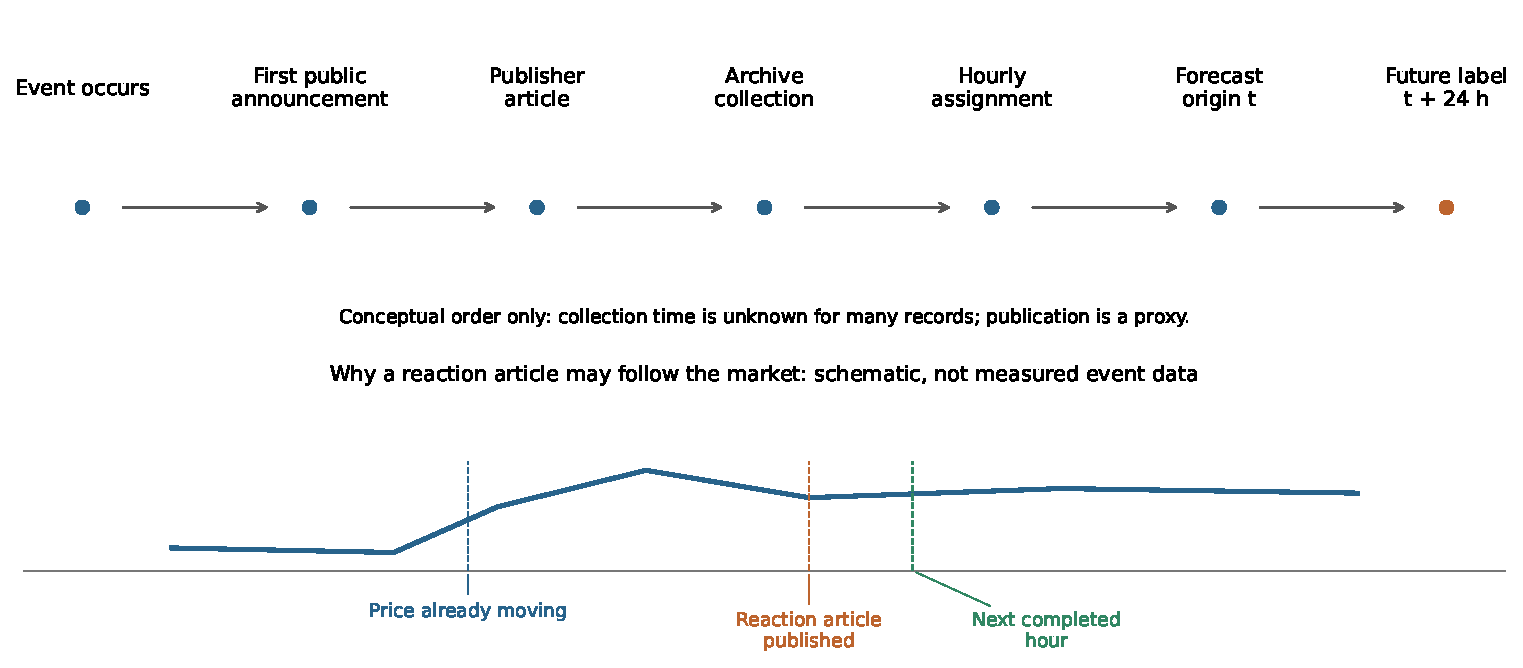
\includegraphics[width=.98\linewidth]{figures/fig02_availability_timeline.pdf}
\caption{Distinction between event occurrence, public announcement, article publication, archive collection and completed-hour assignment. The schematic illustrates possible timing differences; it does not estimate their frequency or duration.}
\label{fig:timeline}
\end{figure}

The study therefore preserves recorded timestamps and assigns headlines forward to completed-hour boundaries. Headlines are never moved to earlier periods on the basis of subsequent price movements.

This procedure prevents direct use of future-dated archived headlines, although it cannot establish the exact first-publication time of every underlying event.

\subsection{Relevance-weighted sentiment decay}
\label{sec:method_decay}

The direct-news configuration uses the average semantic characteristics of headlines recorded within each hour. However, news may remain relevant beyond its publication hour, and older information may have a different relationship with future market behaviour than more recent information.

To examine this possibility, the second news-enhanced configuration (E2) introduces relevance-weighted sentiment decay. This approach combines the sentiment polarity of eligible headlines while assigning greater weight to recent and XRP-specific articles.

The purpose is to test whether a compact representation of recent news performs better than direct hourly news features. It does not assume that news has a known causal effect on prices or that its influence necessarily disappears after a fixed period.

\subsubsection{Construction of the decay features}

For each completed hour $t$, the decay calculation considers headlines assigned within the preceding 48 hours:

\begin{equation}
\mathcal{A}_t
=
\left\{
i:
t-48\mathrm{h}\leq a_i\leq t
\right\}.
\label{eq:decay_window}
\end{equation}

Each eligible article receives a weight determined by two quantities: its XRP specificity and its age relative to the forecast observation.

For half-life $h$, the article weight is

\begin{equation}
w_{i,t}^{(h)}
=
q_i
\exp\left[
-\ln(2)\frac{t-a_i}{h}
\right],
\label{eq:decay_weight}
\end{equation}

where $q_i$ is the XRP-specificity score and $t-a_i$ is the article age in hours.

Four half-lives are evaluated:

\begin{equation}
h\in\{3,6,12,24\}\ \mathrm{hours}.
\label{eq:decay_settings}
\end{equation}

For example, with a six-hour half-life, two equally specific articles published six hours apart receive weights in a ratio of $2:1$, before normalisation. A more recent article therefore contributes more strongly to the aggregated sentiment.

The relevance-weighted sentiment feature is calculated as

\begin{equation}
N_t^{(h)}
=
\frac{
\sum_{i\in\mathcal{A}_t}
w_{i,t}^{(h)}s_i
}{
10^{-9}
+
\sum_{i\in\mathcal{A}_t}
w_{i,t}^{(h)}
}.
\label{eq:decay}
\end{equation}

Here, $s_i$ denotes the GPT-4o sentiment polarity of article $i$. The small constant in the denominator prevents division by zero when no positive relevance weight is available.

A second feature identifies hours in which the trailing archive contains no positive relevance-weighted news mass:

\begin{equation}
M_t^{(h)}
=
\mathbf{1}
\left\{
\sum_{i\in\mathcal{A}_t}
w_{i,t}^{(h)}=0
\right\}.
\label{eq:decay_missing}
\end{equation}

The E2 model receives these two variables, $N_t^{(h)}$ and $M_t^{(h)}$, in addition to the technical inputs.

The absence indicator is important because neutral relevant news and no relevant news can both produce a sentiment value near zero. The indicator allows the forecasting model to distinguish these situations.

The decay equation uses GPT-4o sentiment polarity and XRP specificity. It does not incorporate an additional manually weighted actor-influence, engagement or event-impact formula.

\subsubsection{Illustrative decay calculation}

To demonstrate how the decay features are constructed, Table~\ref{tab:actualdecay} presents the six archived articles eligible at 19 August 2026, 08:00 UTC, using a six-hour half-life.

The example includes all eligible articles, including one with zero XRP specificity. That article contributes no positive relevance weight even though it is present in the archived news.

\begin{table}[htbp]
\centering
\small
\caption{Relevance-weighted sentiment calculation using a six-hour half-life at 19 August 2026, 08:00 UTC.}
\label{tab:actualdecay}
\begin{tabular}{rlrrrrr}
\toprule
Item & Publication UTC & Age (h) & $s_i$ & $q_i$ & Weight & Weighted sentiment \\
\midrule
1 & 17 Aug 10:21 & 45 & $+0.1$ & 0.6 & 0.003315 & $+0.000331$ \\
2 & 17 Aug 18:34 & 37 & $-0.5$ & 1.0 & 0.013920 & $-0.006960$ \\
3 & 18 Aug 06:40 & 25 & $+0.8$ & 1.0 & 0.055681 & $+0.044545$ \\
4 & 18 Aug 09:16 & 22 & $-0.3$ & 1.0 & 0.078745 & $-0.023624$ \\
5 & 18 Aug 16:16 & 15 & $-0.3$ & 0.6 & 0.106066 & $-0.031820$ \\
6 & 19 Aug 07:49 & 0 & $+0.1$ & 0.0 & 0.000000 & $+0.000000$ \\
\bottomrule
\end{tabular}

\par\footnotesize\emph{Note:} Article ages are calculated after rounding publication timestamps forward to completed-hour boundaries. Weights are displayed to six decimal places.
\end{table}

For this example, the total relevance weight and weighted sentiment are

\begin{equation}
\sum_i w_i=0.2577271082,
\qquad
\sum_i w_is_i=-0.0175270789.
\label{eq:decay_example_sums}
\end{equation}

The resulting sentiment feature is

\begin{equation}
N_t^{(6)}
=
\frac{-0.0175270789}
{0.2577271082+10^{-9}}
\approx -0.0680063.
\label{eq:decay_example}
\end{equation}

This calculation reproduces the documented six-hour decay input for the selected observation. It also illustrates a limitation of the representation: a broad market or regulatory article with zero XRP specificity contributes no sentiment weight, even though such information could potentially affect XRP indirectly.

The half-life determines the relative weighting of older and newer articles, not a guaranteed rate at which the aggregated sentiment value itself declines. Because the feature is a normalised weighted average, the common decay factor can largely cancel when the set of eligible articles remains unchanged.

The four decay settings are therefore interpreted as alternative recency-weighting assumptions. Their forecasting performance is compared using validation data, rather than selecting a half-life by visually matching historical price movements.

\subsection{Early fusion and BiLSTM forecasting network}
\label{sec:method_predictor}

The final stage combines the prepared inputs and generates the 24-hour XRP return forecast.

The study uses early fusion, meaning that technical and news features are joined at each observed hour before being processed by the recurrent network. This allows the model to learn relationships between market conditions and news information within the same historical sequence.

For example, a positive XRP-related headline may occur during an upward price trend, a period of high volatility or a period of relatively stable trading. Early fusion allows the model to examine these combinations rather than interpreting news sentiment independently of the market environment.

The three experimental input representations are

\begin{equation}
\mathbf{x}_t^{E0}
=
\mathbf{T}_t
\in\mathbb{R}^{19},
\label{eq:e0_input}
\end{equation}

\begin{equation}
\mathbf{x}_t^{E1B}
=
\left[
\mathbf{T}_t;
\mathbf{D}_t
\right]
\in\mathbb{R}^{25},
\label{eq:e1b_input}
\end{equation}

and

\begin{equation}
\mathbf{x}_t^{E2}
=
\left[
\mathbf{T}_t;
N_t^{(h)};
M_t^{(h)}
\right]
\in\mathbb{R}^{21}.
\label{eq:e2_input}
\end{equation}

Accordingly, each 30-hour historical input window has one of the following dimensions:

\begin{equation}
\mathbf{X}_t^{E0}\in\mathbb{R}^{30\times19},
\qquad
\mathbf{X}_t^{E1B}\in\mathbb{R}^{30\times25},
\qquad
\mathbf{X}_t^{E2}\in\mathbb{R}^{30\times21}.
\label{eq:input_dimensions}
\end{equation}

These configurations use the same recurrent architecture design but are trained independently. The term \emph{shared architecture} therefore refers to a common network structure, not to a single set of fitted weights shared across the experiments.

Figure~\ref{fig:flow} illustrates the complete forecasting pipeline.

\begin{figure}[htbp]
\centering
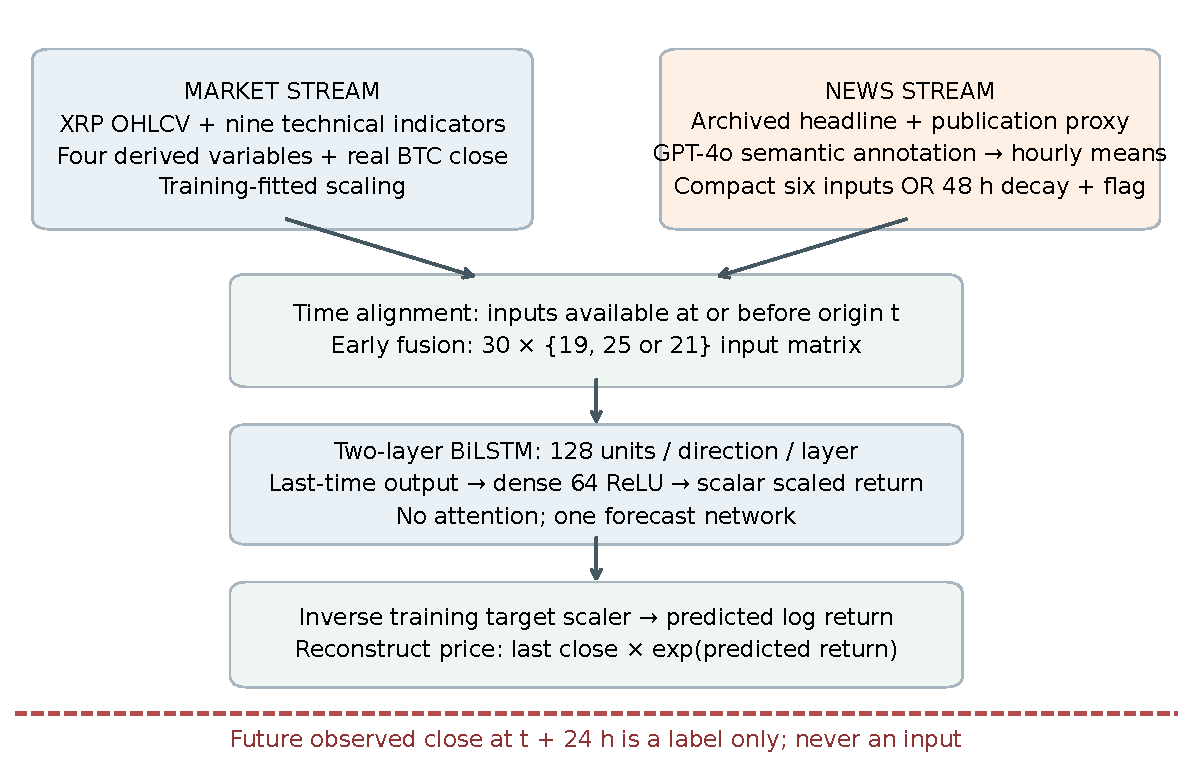
\includegraphics[width=.98\linewidth]{figures/fig01_architecture.pdf}
\caption{Proposed forecasting framework. Historical market observations and time-aligned news features are combined before entering a BiLSTM predictor. The technical-only and news-enhanced configurations use the same architecture design but are trained separately. All input observations occur at or before the forecast origin.}
\label{fig:flow}
\end{figure}

\subsubsection{BiLSTM architecture}

The forecasting model uses a Bidirectional Long Short-Term Memory network. LSTM networks were developed to represent sequential relationships using memory states that regulate information retention and updating \citep{Hochreiter1997}. Bidirectional recurrence extends this approach by processing an observed sequence in both forward and backward directions \citep{Schuster1997}.

In the present application, both directions operate exclusively within the 30-hour historical window. The backward direction does not access observations from the future 24-hour forecasting period.

The implemented architecture contains two stacked bidirectional LSTM layers. Each layer uses 128 hidden units per direction, producing 256-dimensional bidirectional outputs. Dropout with probability $0.2$ is applied between the recurrent layers.

The model reads the output at the final input time step. This representation is passed to a fully connected layer with 64 units and Rectified Linear Unit (ReLU) activation, followed by dropout with probability $0.2$ and a final linear layer producing one scalar forecast.

The architecture can be summarised as

\begin{equation}
\mathbf{X}_t
\longrightarrow
\mathrm{BiLSTM}_{128}
\longrightarrow
\mathrm{BiLSTM}_{128}
\longrightarrow
\mathrm{Dense}_{64}
\longrightarrow
\widehat{z}_t.
\label{eq:network_architecture}
\end{equation}

The scalar output $\widehat{z}_t$ represents the predicted scaled 24-hour log return. It is converted back to the original return scale and, where required, reconstructed as a future XRP closing price using Equation~\ref{eq:inverse}.

The network uses a final-time output readout rather than attention or pooling across all time steps. In particular, the final-time bidirectional output should not be interpreted as a symmetric concatenation of both full-window terminal directional states. Nevertheless, the stacked bidirectional layers allow information from different positions in the historical window to contribute to the learned representation.


The proposed framework therefore provides a consistent forecasting architecture for evaluating alternative input representations. The technical-only configuration establishes the baseline, while the direct-news and sentiment-decay configurations introduce different representations of GPT-4o-derived information. The experimental configurations, training procedures, baseline comparisons and evaluation methodology are described in Section~\ref{sec:experiments}.


\section{Experimental Design and Results}
\label{sec:experiment-evaluation}
\label{sec:experiments}

This section evaluates whether incorporating GPT-4o-derived news information improves the 24-hour forecasting of XRP/USDT closing prices beyond technical and market information. The empirical analysis proceeds from technical-only forecasting to controlled news-feature comparisons, then to later-period evaluation and model interpretability. To preserve comparability, results are grouped by experimental protocol: models are ranked together only when they share the relevant forecast origins, target timestamps and evaluation definition. Earlier architecture studies provide supporting evidence but are not pooled with the principal E0--E4 feature comparison.

\subsection{Research Questions and Evaluation Framework}
\label{subsec:research-questions}

The analysis follows the five research questions introduced in Section~\ref{sec:introduction}. RQ1 establishes the technical reference and examines the supporting LSTM/BiLSTM and Bitcoin-input comparisons. RQ2 tests the incremental value of direct news, including its later-period performance. RQ3 compares direct features with the four predefined decay settings. RQ4 examines exploratory market/news conditions and publication timing, with the conditional-risk results retained in Appendix~\ref{app:additional}. RQ5 concerns model attribution and the separate HBAR transfer experiment. The results below follow this sequence while keeping experiments with different fitting targets separate.

The principal comparison is \emph{E0 versus E1B}. Both models use the same historical XRP and BTC observations, the same 30-hour input length, the same 24-hour log-return target, the same chronological partitions, the same five seeds and the same training procedure. E0 receives technical and market inputs; E1B adds six hourly news-related features. The common BiLSTM design is preserved, although its input-dependent parameter count increases slightly when news variables are added. This matched design supports a focused test of incremental news information without conflating it with a different target or market period.

\subsection{Data, Forecasting Task and Experimental Controls}
\label{subsec:experimental-protocol}

\subsubsection{Data and chronological evaluation}

\noindent\textbf{Research materials.} Dataset definitions, source code, frozen configurations and saved prediction outputs are documented at \ResearchRepository. News-source text remains subject to the original providers' redistribution terms; acquisition instructions and the permitted derived numerical inputs should be used where full-text redistribution is restricted.

The prepared dataset contains 26,337 hourly XRP/USDT observations spanning October 2023 to October 2026, together with BTC/USDT closing prices and the technical features defined in the methodology section. The news archive contains 19,928 records, processed into hourly features using the recorded publication times. Each article is eligible for a forecast only after its archived timestamp has become available in the completed-hour feature sequence. News features are not backfilled using future article publication times.

The main matched experiment uses 18,861 training origins, 2,136 validation origins and 5,262 later evaluation origins. Validation covers 19 December 2025, 07:00 UTC, to 18 March 2026, 06:00 UTC; the later evaluation covers 19 March 2026, 07:00 UTC, to 24 October 2026, 12:00 UTC. Chronological boundaries are purged so that training labels do not overlap validation target periods. All input and target scaling parameters are fitted on training information only.

\begin{table}[!htbp]
\centering\small
\caption{Chronological design of the principal matched XRP experiments. All configurations within this programme use identical forecast origins and exactly 24-hour target timestamps.}
\label{tab:main_partitions}
\begin{tabular}{lrl}
\toprule
Partition & Origins & Role in evaluation \\
\midrule
Training & 18,861 & Model fitting and scaler estimation \\
Validation & 2,136 & Checkpoint and configuration selection \\
Later retrospective evaluation & 5,262 & Frozen E0/E1B performance assessment \\
\bottomrule
\end{tabular}
\end{table}

The later block is reserved from fitting and checkpoint selection for the final E0/E1B comparison. It is termed \emph{retrospective} because the broader historical period had been examined during the development of the research programme; it is not represented as a prospective live-trading test.

\subsubsection{Target, baselines and performance measures}

For an observed closing price $P_t$, each neural model receives the preceding 30 completed hourly feature vectors and predicts the logarithmic 24-hour return
\begin{equation}
 r_{t,24}=\log\!\left(\frac{P_{t+24}}{P_t}\right),
 \qquad
 \widehat P_{t+24}=P_t\exp(\widehat r_{t,24}).
 \label{eq:exp_target}
\end{equation}
The predicted return is inverse-scaled and converted back to a price before calculating the reported metrics. Bidirectional recurrence processes only the observed input window; it does not use future candles. The deterministic persistence benchmark predicts $\widehat P_{t+24}^{\mathrm{pers}}=P_t$ on exactly the same forecast origins.

The primary selection criterion is price-scale root mean squared error (RMSE). Mean absolute error (MAE), coefficient of determination ($R^2$) and directional accuracy provide complementary assessments:
\begin{align}
\mathrm{RMSE}&=\sqrt{\frac{1}{N}\sum_{t=1}^{N}(P_{t+24}-\widehat P_{t+24})^2}, \\
\mathrm{MAE}&=\frac{1}{N}\sum_{t=1}^{N}|P_{t+24}-\widehat P_{t+24}|,\\
R^2&=1-\frac{\sum_t(P_{t+24}-\widehat P_{t+24})^2}
{\sum_t(P_{t+24}-\overline P)^2}.
\label{eq:exp_metrics}
\end{align}
Directional accuracy compares the signs of observed and predicted price changes. Because persistence predicts zero movement, it is not assigned an up/down directional accuracy in the main tables. Price-level $R^2$ is reported alongside RMSE rather than used alone to establish forecasting skill.

\subsubsection{Training and architecture consistency}

E0--E3 share two stacked BiLSTM layers with 128 hidden units per direction, dropout $0.2$, a 64-unit ReLU dense layer and one scalar output. The network uses the final recurrent representation, without attention. E0 has 19 technical and market inputs, including BTC close, and 564,353 parameters. E1B has 25 inputs and 570,497 parameters. The 1.09\% parameter increase follows from the additional input columns; the architecture and optimisation design remain the same.

Five fixed seeds ($42$, $123$, $2026$, $7$ and $99$) are used throughout the matched neural experiments. Models are trained with Adam (learning rate $0.001$), batch size 32, at most 200 epochs and early-stopping patience 15. The checkpoint minimising validation scaled-return mean squared error is retained. Input RobustScaler and target MinMaxScaler transformations are fitted using training observations only. Validation rankings use the arithmetic mean of the five separately calculated seed RMSE values, not the best seed and not an ensemble forecast.

The principal programme evaluates ten configurations at five seeds each, comprising 40 newly trained and ten preserved E0/E1 runs. The complete ranking retains all 50 configuration--seed outcomes. E4 differs from E0--E3 by using a separate 16-unit GRU correction network on frozen, seed-matched E0 predictions and is therefore identified explicitly as a different model family.

\subsection{Technical-Only Forecasting: Establishing the Reference}
\label{subsec:technical-only-results}

\subsubsection{Matched E0 and persistence comparison}

The primary technical reference is E0, trained using the same target, dates and optimisation protocol as the subsequent news-enhanced models. Across five seeds on the 2,136-origin validation block, E0 achieved RMSE $0.063935$ USDT, MAE $0.044514$ USDT, $R^2=0.951957$ and directional accuracy $53.78\%$. Persistence achieved RMSE $0.064962$ USDT and MAE $0.044774$ USDT on the same targets. E0 therefore reduced validation RMSE by $1.58\%$ relative to persistence.

\begin{table}[!htbp]
\centering\small
\caption{Apples-to-apples technical reference on the common 2,136-origin validation block. E0 is the five-seed mean; persistence is deterministic. All targets are exactly 24 hours ahead.}
\label{tab:technical_matched_reference}
\begin{tabular}{lrrrr}
\toprule
Model & RMSE (USDT) & MAE (USDT) & $R^2$ & Direction (\%) \\
\midrule
E0 technical-only BiLSTM & \textbf{0.063935} & \textbf{0.044514} & \textbf{0.951957} & 53.78 \\
Persistence & 0.064962 & 0.044774 & 0.950403 & -- \\
\bottomrule
\end{tabular}
\end{table}

This result defines the technical reference against which news representations are evaluated. It is a comparison of the same price targets, rather than a comparison of unrelated historical model scores.

\subsubsection{Supporting technical architecture comparison}

A separate controlled technical-only experiment compared BiLSTM, unidirectional LSTM, a near-parameter-matched wider LSTM, ARIMAX and persistence on 5,262 common later-period price targets. This experiment used direct-price or log-price fitting objectives rather than the main E0--E4 log-return objective. Its results are therefore interpreted \emph{within that experiment only} and are not inserted into the E0--E4 ranking.

\begin{table}[!htbp]
\centering\small
\caption{Supporting technical-only architecture experiment on common later-period price targets. Neural values are means of five runs; ARIMAX and persistence are single-fit/deterministic comparators. This is a distinct training-target experiment from the matched E0--E4 study.}
\label{tab:technical_architecture_context}
\fitTable{%
\begin{tabular}{lrrrr}
\toprule
Model & RMSE (USDT) & Seed SD & MAE (USDT) & $R^2$ \\
\midrule
Persistence & \textbf{0.03934} & -- & 0.02675 & \textbf{0.93723} \\
Technical ARIMAX & 0.03945 & -- & \textbf{0.02673} & 0.93690 \\
BiLSTM with BTC & 0.05682 & 0.00996 & 0.04380 & 0.86584 \\
LSTM 128 with BTC & 0.06026 & 0.01292 & 0.04619 & 0.84735 \\
LSTM 210 with BTC & 0.06356 & 0.01449 & 0.05103 & 0.82934 \\
BiLSTM without BTC & 0.07027 & 0.00965 & 0.05811 & 0.79675 \\
\bottomrule
\end{tabular}}
\end{table}

Among the recurrent networks in this supporting experiment, BiLSTM with BTC had $5.70\%$ lower mean RMSE than LSTM 128 and $10.61\%$ lower mean RMSE than LSTM 210. The latter was designed as an approximate parameter-capacity comparison (562,089 versus 564,353 parameters). Removing BTC increased the BiLSTM's RMSE, supporting the inclusion of broader cryptocurrency-market context. ARIMAX and persistence achieved lower RMSE than the recurrent models in this separate price-target experiment. These observations motivate the selected BiLSTM architecture without implying that the numerical scores of different target-fitting protocols are interchangeable.

The wider archive also contains a GARCH volatility evaluation. Because its outcome is conditional variance rather than the future closing price, its variance errors are not included in the price-forecast ranking. No unverified SVM, plain-RNN or EGARCH price results are added.

\noindent\textbf{RQ1 finding.} The matched technical-only BiLSTM modestly improved upon persistence during validation. In a separate technical architecture study, BiLSTM outperformed the tested LSTM alternatives, while statistical and naive methods remained strong comparators. These results establish a well-defined technical reference for the incremental news experiment.


\subsection{Incremental Forecasting Value of News Features}
\label{subsec:news-representation-results}

\subsubsection{News configurations and controlled comparisons}

The main experiment compares alternative ways of representing GPT-4o-derived information within the fixed forecasting task. E1 is a preserved earlier direct-news construction with eight news-related inputs. E1B is the compact direct-news model with six inputs: hourly means of GPT-4o polarity, XRP specificity, XRP stance and uncertainty, plus news presence and capped recency. E2 introduces a specificity-weighted, trailing 48-hour sentiment representation using the predefined half-lives $h\in\{3,6,12,24\}$ hours (Equation~\eqref{eq:decay}). E3 combines E1B with the six-hour E2 representation. E4 applies gated or ungated GRU corrections to frozen E0 forecasts.

\begin{table}[!htbp]
\centering\small
\caption{Model families evaluated on the same 2,136 XRP validation origins. E0--E3 retain the shared BiLSTM design; E4 is a separately identified frozen-base correction model.}
\label{tab:matched_configuration_design}
\begin{tabular}{lp{6.7cm}r}
\toprule
Configuration & Representation & Input width \\
\midrule
E0 & Technical and market information only & 19 \\
E1 & Preserved earlier direct-news features & 27 \\
E1B & Six compact direct-news features & 25 \\
E2 ($h=3,6,12,24$) & Two decay-related news features & 21 \\
E3 & E1B combined with E2 ($h=6$) & 27 \\
E4 gated/ungated & GRU news correction to frozen E0 & Separate \\
\bottomrule
\end{tabular}
\end{table}

All configurations use the same origin and target timestamps, so the observed differences are attributable to the tested model-and-feature configurations rather than to changing the evaluation sample. The most direct incremental-news comparison is E0 versus E1B, which preserves the network design and changes the input representation. Comparisons involving E4 also change the correction architecture and are interpreted as alternative system designs rather than pure feature ablations. The older E1 construction differs from E1B in news preparation as well as feature width, so E1 versus E1B is not described as an isolated feature-count experiment.

\subsubsection{Matched validation results}

Table~\ref{tab:Table1} gives the complete ranking. The percentage improvement relative to the technical-only control is
\begin{equation}
G_m=100\left(1-\frac{\overline{\mathrm{RMSE}}_m}{\overline{\mathrm{RMSE}}_{E0}}\right),
\label{eq:validation_gain}
\end{equation}
where each bar denotes the arithmetic mean of five individual-seed RMSE values. Positive $G_m$ indicates lower validation error than E0.

\begin{table}[!htbp]
\centering\small
\caption{Complete matched XRP validation ranking: 2,136 identical origins, exact 24-hour targets and five seeds per neural configuration. SD measures between-seed variation; it is not a confidence interval over independent market periods.}
\label{tab:Table1}
\fitTable{%
\begin{tabular}{lrrrrrr}
\toprule
Configuration & RMSE & Seed SD & MAE & $R^2$ & Direction (\%) & Gain vs E0 (\%) \\
\midrule
E1B compact news & \textbf{0.063036} & 0.000385 & \textbf{0.043989} & \textbf{0.953299} & \textbf{55.87} & +1.406 \\
E4 ungated & 0.063474 & 0.000501 & 0.044355 & 0.952646 & 53.91 & +0.720 \\
E2 $h=6$ & 0.063637 & 0.000768 & 0.044611 & 0.952400 & 54.04 & +0.466 \\
E4 gated & 0.063646 & 0.000475 & 0.044498 & 0.952389 & 52.81 & +0.451 \\
E2 $h=3$ & 0.063724 & 0.000660 & 0.044432 & 0.952272 & 52.28 & +0.330 \\
E1 earlier news & 0.063883 & 0.000854 & 0.044766 & 0.952030 & 54.59 & +0.081 \\
E3 combined & 0.063924 & 0.001023 & 0.045195 & 0.951965 & 53.34 & +0.017 \\
E0 technical-only & 0.063935 & 0.000416 & 0.044514 & 0.951957 & 53.78 & 0.000 \\
E2 $h=12$ & 0.064019 & 0.001314 & 0.044839 & 0.951816 & 53.74 & -0.131 \\
E2 $h=24$ & 0.064341 & 0.000992 & 0.044975 & 0.951337 & 50.72 & -0.635 \\
Persistence & 0.064962 & -- & 0.044774 & 0.950403 & -- & -- \\
\bottomrule
\end{tabular}}
\end{table}

E1B achieved the lowest validation RMSE ($0.063036$ USDT), a $1.406\%$ reduction from E0 ($0.063935$ USDT), together with lower MAE and higher directional accuracy ($55.87\%$ versus $53.78\%$). Relative to persistence, E1B's numerical RMSE reduction was approximately $2.96\%$. These are performance differences on the common validation period, not evidence of a separate news-only forecasting capability.

Among decay variants, the six-hour half-life was best ($0.063637$ USDT), but it did not outperform compact direct news. The E3 combination produced nearly the same RMSE as E0. The ungated and gated E4 corrections improved numerically over E0 but did not surpass E1B. Thus, greater feature or model complexity did not consistently improve validation accuracy. The E2 normalised weighted average changes the relative weighting of available articles; it is not a calibrated causal price-impact coefficient.

\begin{figure}[!htbp]
\centering
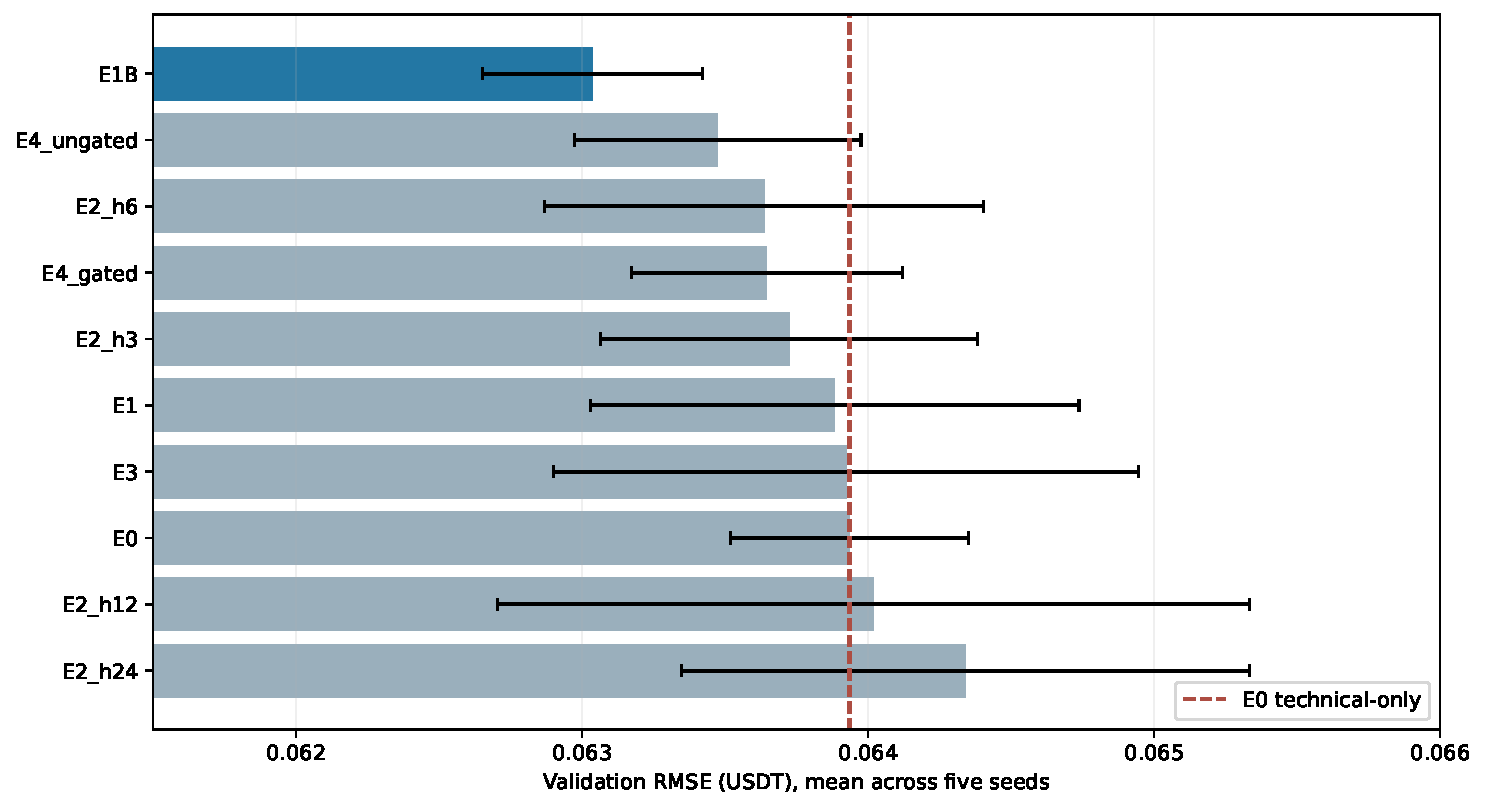
\includegraphics[width=.96\linewidth]{figures/new_validation_ranking.pdf}
\caption{Matched validation RMSE ranking for ten configurations. Bars show five-seed mean RMSE values and error bars show between-seed standard deviations. The dashed vertical line marks the technical-only E0 reference. The RMSE axis is truncated to resolve the small differences between configurations.}
\label{fig:validation_rank}
\end{figure}

Figure~\ref{fig:validation_rank} shows that E1B ranks first on validation, although several configurations occupy a narrow RMSE range. The plotted error bars describe sensitivity to neural training initialisation and do not replace the paired time-series uncertainty analysis below.

\begin{figure}[!htbp]
\centering
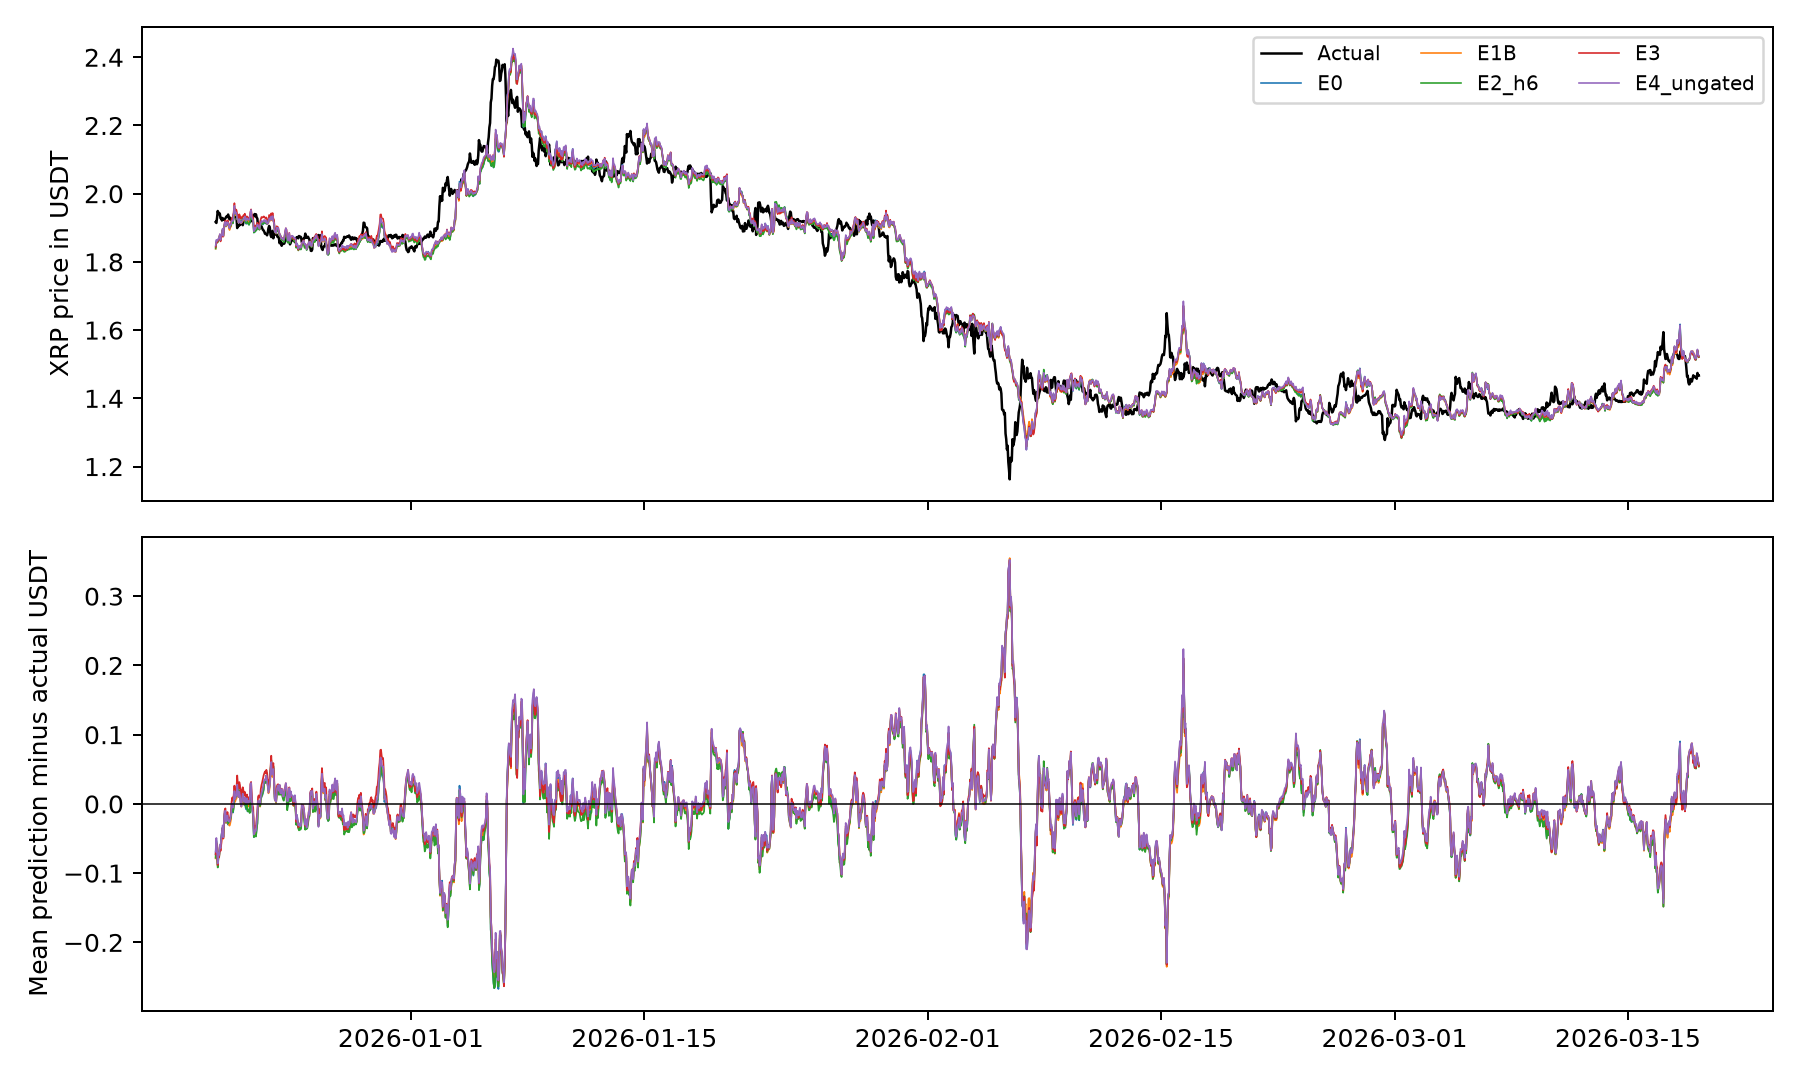
\includegraphics[width=\linewidth]{figures/validation_predictions.png}
\caption{Common-period XRP validation predictions for representative configurations. The upper panel plots observed prices and the mean prediction across five seeds; the lower panel plots mean prediction minus observed price. These mean curves are visual summaries only: Table~\ref{tab:Table1} reports the mean of the five individually evaluated seed metrics, not the performance of a prediction ensemble.}
\label{fig:validation_predictions}
\end{figure}

The price trajectories in Figure~\ref{fig:validation_predictions} show that the models track broad movements but can exhibit larger errors around abrupt changes. The residual panel complements the aggregate metrics by making those periods visible. The close visual agreement between model curves is consistent with the relatively small differences in validation RMSE.


\subsection{Statistical Robustness and Later-Period Generalisation}
\label{subsec:robustness-and-generalisation}

\subsubsection{Validation uncertainty and model selection}

Hourly 24-hour-ahead forecasts overlap in their outcome intervals, so their errors are serially dependent. The primary uncertainty analysis therefore uses 2,000 paired circular moving-block bootstrap resamples \citep{Kunsch1989}, with a 72-hour block length and sensitivity checks at 24 and 168 hours. The paired estimand is the difference in the square root of seed-averaged squared errors, rather than the difference between arithmetic mean seed RMSEs. This preserves the pairing of model errors at each forecast origin while accounting for temporal dependence.

Stage-specific multiplicity adjustments were applied to the predeclared contrasts: a 99.5\% interval in the initial ten-contrast stage, 98.75\% in the four-contrast E3 stage and approximately 99.286\% in the seven-contrast E4 stage. The E1B-versus-E0 comparison had a favourable unadjusted 95\% interval, but its multiplicity-adjusted interval included zero. E1B also outperformed E0 in only two of four calendar-month validation segments. E1B is therefore designated the \emph{validation-selected candidate} on mean RMSE, rather than a statistically established improvement under the adjusted comparisons.

\subsubsection{Frozen retrospective evaluation}

The validation-selected E1B configuration and the matched E0 control were then assessed using their saved checkpoints on 5,262 later forecast origins. Model weights, feature definitions and training scalers were not refitted using later evaluation targets. The comparison retains the same 24-hour return target and the same origin timestamps for E0, E1B and persistence.

\begin{table}[!htbp]
\centering\small
\caption{Later reserved retrospective XRP evaluation on 5,262 identical origins. Neural values are arithmetic means across five saved seeds; SD reflects seed variability. All RMSE and MAE values are in USDT.}
\label{tab:final}
\fitTable{%
\begin{tabular}{lrrrr}
\toprule
Model & Mean RMSE $\pm$ seed SD & MAE & $R^2$ & Direction (\%) \\
\midrule
Persistence & \textbf{0.039341} & \textbf{0.026753} & \textbf{0.937234} & -- \\
E0 technical-only & $0.039976\pm0.000239$ & 0.027432 & 0.935191 & 49.60 \\
E1B compact news & $0.042118\pm0.004186$ & 0.028314 & 0.927493 & 49.44 \\
\bottomrule
\end{tabular}}
\end{table}

The later evaluation reverses the validation ordering. E1B had $5.358\%$ higher arithmetic mean-seed RMSE than E0 ($0.042118$ versus $0.039976$ USDT). Persistence achieved the lowest RMSE ($0.039341$ USDT). E1B also had higher MAE and lower directional accuracy than E0. All five seeds remain included, including E1B seed 42, which produced later-period RMSE $0.049553$ USDT and contributed to the larger E1B seed dispersion.

\begin{figure}[!htbp]
\centering
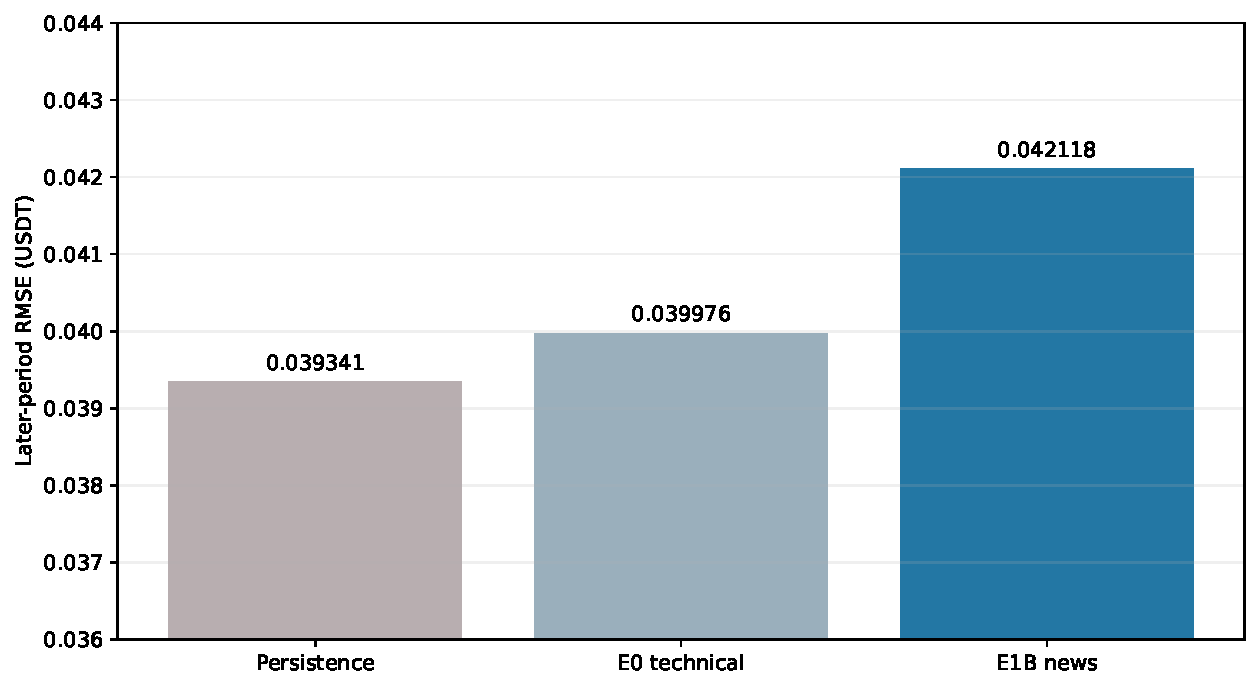
\includegraphics[width=.86\linewidth]{figures/new_final_comparison.pdf}
\caption{Later retrospective RMSE on identical XRP target prices. The bars show persistence and arithmetic mean RMSE across the five saved E0 and E1B checkpoints. The vertical axis begins above zero to resolve the differences; values are labelled above the bars.}
\label{fig:final_comparison}
\end{figure}

Figure~\ref{fig:final_comparison} makes the change in model ordering explicit. Absolute RMSE is lower in this period than during validation, but the market observations and price dynamics differ; the meaningful comparison is the relative performance of models on the \emph{same} later-period observations.

The primary 72-hour paired moving-block bootstrap produced an E1B-minus-E0 RMSE-risk difference of $+0.002307$ USDT, with a 95\% interval of $[0.000601,\,0.004255]$. The corresponding risk-estimand deterioration was $5.772\%$, slightly different from the $5.358\%$ comparison of arithmetic mean seed RMSEs because averaging and square-root operations are performed in a different order. The 24- and 168-hour block sensitivity intervals also favoured E0. A supplementary Newey--West HAC comparison of paired squared-error differences \citep{Newey1987} reported $p=0.0386$ using 71 lags.

The paired results support the observed later-period ranking in favour of E0. They do not imply that the same ranking will necessarily hold in every future regime. As an additional timing sensitivity check, the frozen E1B model was evaluated with 1-, 6- and 24-hour delays applied to news availability. The resulting RMSE values remained close to the original E1B score and did not reverse the comparison with E0. These delayed-input scenarios are diagnostic stress tests, not additional candidates selected on the later period.

\noindent\textbf{RQ2 and RQ3 findings.} Compact direct news achieved the best numerical validation performance, but the adjusted validation analysis did not establish a robust gain. On the later reserved retrospective block, the matched technical-only model and persistence both outperformed E1B. The experiment therefore identifies a validation-specific benefit that did not persist in the evaluated later market period.


\subsection{Feature Attribution and Interpretability}
\label{subsec:feature-attribution}
\label{subsec:shap-analysis}

To examine whether the saved E1B networks respond to the additional inputs, the study applies \emph{expected integrated gradients} (EIG) \citep{Sundararajan2017}. This method is distinct from exact SHAP or combinatorial Shapley-value estimation. The explained output is the inverse-scaled predicted 24-hour log return, before reconstruction into price. For an input $x$, a training reference $b$, feature $j$ and historical lag $\ell$, the attribution is
\begin{equation}
\mathrm{EIG}_{\ell j}(x)=
\mathbb E_{b}\!\left[
(x_{\ell j}-b_{\ell j})
\int_0^1
\left.\frac{\partial f(u)}{\partial u_{\ell j}}\right|_{u=b+\alpha(x-b)}
\,d\alpha
\right],
\label{eq:eig}
\end{equation}
where $f$ denotes the saved model's inverse-scaled predicted-return function. Attributions are aggregated in absolute value over the 30 historical lags and averaged over forecast origins.

The verification uses all five E1B checkpoints, two frozen training-reference sets per seed, 32 references per set and 1,000 fixed forecast origins per pass, yielding 10,000 explanations. Adaptive Gauss--Legendre integration uses 64, 128 or 256 quadrature points as needed. Of the 10,000 explanations, 9,948 met the stated completeness tolerance and 52 retained explanations did not; no seed or reference set was discarded. The global percentages are the equal-pass mean of absolute attribution shares.

\begin{table}[!htbp]
\centering\small
\caption{Verified EIG attribution shares for saved E1B models. The news group includes four GPT-derived semantic fields and two locally constructed news-availability fields.}
\label{tab:eig_attribution}
\begin{tabular}{lr}
\toprule
Input group & Mean absolute attribution share \\
\midrule
Technical and market features & \textbf{76.89\%} \\
News-related features & 23.11\% \\
\bottomrule
\end{tabular}
\end{table}


\begin{figure}[!htbp]
\centering
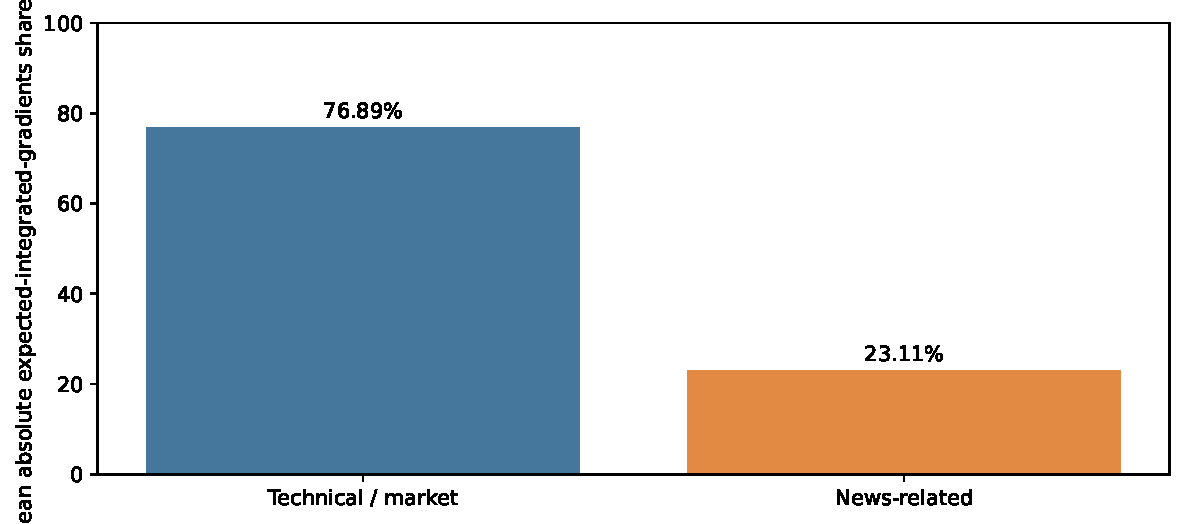
\includegraphics[width=.82\linewidth]{figures/new_attribution.pdf}
\caption{Verified expected-integrated-gradients shares for the saved E1B checkpoints: 76.89\% technical/market and 23.11\% news-related inputs. These are relative absolute attribution shares for predicted returns, not proportions of observed price movement or forecasting accuracy gains.}
\label{fig:attribution}
\end{figure}

The attribution result establishes that E1B's fitted forecasting function is sensitive to both market and news-related variables. The news group includes publication presence and recency, so its share cannot be interpreted as semantic sentiment alone. News attribution ranged from 18.45\% to 31.32\% across the ten seed--reference passes; the alternative pooled calculation yielded 22.82\%. These diagnostics characterise sensitivity to reference choice and model initialisation. The residual completeness exceptions are retained in the reported calculation.

Crucially, attribution measures how the model uses an input, not whether that input improves future predictions. The later-period forecasting results and the EIG results are therefore consistent: a model can respond measurably to news features while forecasting less accurately than its technical-only control.

\noindent\textbf{RQ5 attribution finding.} Technical and market variables account for approximately three-quarters of E1B's mean absolute attribution, while news-related variables account for approximately one-quarter under the verified EIG design. This establishes measurable model use of news information, without implying causal market influence or superior forecast performance.


The separate HBAR experiment addresses the cross-asset part of RQ5 and is reported in Section~\ref{sec:hbar-transfer}. Its results are kept outside the XRP model ranking because the asset, price scale and asset-specific news coverage differ.

\subsection{Synthesis of the Research Findings}
\label{subsec:experimental-synthesis}

The experiments provide a coherent sequence of evidence. The matched technical-only E0 model established the reference for incremental news evaluation and modestly improved upon persistence during validation. A separate architecture comparison showed that BiLSTM was competitive among the evaluated recurrent technical models, while ARIMAX and persistence remained strong statistical and naive benchmarks. These two experiment families were kept separate because their model-fitting targets differed.

On the principal matched validation block, compact direct-news E1B achieved the lowest RMSE among ten configurations, with a $1.406\%$ numerical reduction relative to E0. Neither the tested sentiment-decay equations nor the combined and GRU-correction alternatives improved upon E1B. The paired, multiplicity-adjusted validation analysis did not establish a robust advantage from the selected news representation.

The later retrospective evaluation reversed the validation ordering: E1B had $5.358\%$ higher arithmetic mean-seed RMSE than E0, while persistence performed best. Dependence-aware paired intervals supported the later-period comparison. EIG nevertheless attributed $23.11\%$ of absolute model sensitivity to news-related inputs, demonstrating that the model used the additional features even when they did not improve its evaluated forecasts. The HBAR transfer check likewise showed no forecasting benefit from the transferred news representation; the limited asset-specific coverage is examined separately in Section~\ref{sec:hbar-transfer}.

The central finding is therefore a distinction between \emph{successful integration of news information into a forecasting network} and \emph{demonstrated generalisable forecasting improvement}. The proposed framework accomplishes the former and exhibits a small numerical validation benefit, but the available later-period evidence does not establish the latter. For RQ4, the exploratory conditional-risk analyses in Appendix~\ref{app:additional} identify no multiplicity-adjusted forecasting improvement in the examined strata. The timing and coverage of archived news are discussed in Section~\ref{sec:discussion}; these diagnostics do not establish causal news effects.


% ============================================================
% SECTION 5: SECONDARY CROSS-ASSET EVALUATION
% ============================================================

\FloatBarrier
\section{Secondary Cross-Asset Evaluation: HBAR}
\label{sec:hbar-transfer}

To assess the transferability of the proposed news representation, a separate experiment was conducted using Hedera (HBAR). XRP remained the primary research asset, while HBAR provided an additional evaluation of whether the compact news representation selected during XRP validation could generalise without asset-specific retuning. The experiment used the shared cryptocurrency and ISO 20022-related news watchlist, which includes asset-specific, regulatory, policy and broader market developments. Inclusion in this watchlist represents the scope of news collection and does not imply that any cryptocurrency holds ISO certification.

The HBAR experiment followed the principal forecasting protocol. Technical indicators were derived independently from HBAR OHLCV observations, while BTC closing prices provided common market context. The models used identical validation dates, 30-hour historical sequences, exact 24-hour log-return targets, chronological partitions and five training seeds. All HBAR transformations were fitted exclusively on the corresponding HBAR training data.

\subsection{Cross-Asset Forecasting Performance}
\label{subsec:hbar-performance}

Table~\ref{tab:hbar-results} presents the HBAR validation results across 2,136 matched forecast origins. The transferred news representation increased mean RMSE by 2.060\% relative to the HBAR technical-only model, while persistence achieved the lowest RMSE among the evaluated HBAR configurations.

\begin{table}[!htbp]
\centering\small
\caption{HBAR validation results across 2,136 matched forecast origins. Neural results are five-seed means; standard deviations reflect training-seed variability. Errors are expressed in USDT per HBAR.}
\label{tab:hbar-results}
\fitTable{%
\begin{tabular}{lrrrr}
\toprule
Model & RMSE mean $\pm$ SD & MAE & $R^2$ & Directional accuracy (\%) \\
\midrule
Technical-only & $0.0037095 \pm 0.0000423$ & 0.0028132 & 0.881438 & 53.16 \\
Transferred news & $0.0037860 \pm 0.0000520$ & 0.0028592 & 0.876497 & 53.11 \\
Persistence & \textbf{0.0036900} & 0.0028151 & \textbf{0.882699} & -- \\
\bottomrule
\end{tabular}}
\end{table}

The primary 72-hour paired moving-block bootstrap produced a hybrid-minus-technical RMSE-risk confidence interval of $[0.00000709,\,0.00014937]$ USDT, favouring the technical-only configuration. Thus, the compact news representation selected using XRP validation did not provide an incremental forecasting advantage when transferred directly to HBAR. This is a separate validation transfer experiment rather than an additional final-period evaluation. Absolute RMSE values should not be compared directly between XRP and HBAR because their price scales differ substantially.

\subsection{News Coverage and Transferability}
\label{subsec:hbar-coverage}

To contextualise the transfer results, the shared news archive was examined for explicit asset-name coverage. Across the dataset period, 118 headlines explicitly mentioned HBAR or Hedera, compared with 11,428 headlines mentioning XRP or Ripple. Within the 2,136 validation origins, only 216 origins (10.11\%) had an explicit HBAR/Hedera headline in the preceding 48 hours. Under the same archive definition, all XRP validation origins had an explicit XRP/Ripple headline within that historical window. HBAR-specific coverage was therefore considerably sparser in the collected corpus.

The combination of limited HBAR-focused reporting and XRP-oriented semantic annotations offers a plausible explanation for the weaker transfer performance. Nevertheless, the experiment does not isolate the individual effects of coverage quantity, annotation relevance or market-specific information content. It also does not establish a minimum news-volume threshold for successful forecasting. Determining whether improved HBAR-specific coverage would enhance predictive accuracy requires a separately annotated HBAR corpus and a controlled experiment.

Figure~\ref{fig:hbar-transfer} presents the forecasting comparison alongside the 48-hour headline-coverage diagnostic. Together, these findings illustrate why asset-specific information relevance must be considered when transferring news-enhanced forecasting models.

\begin{figure}[!htbp]
\centering
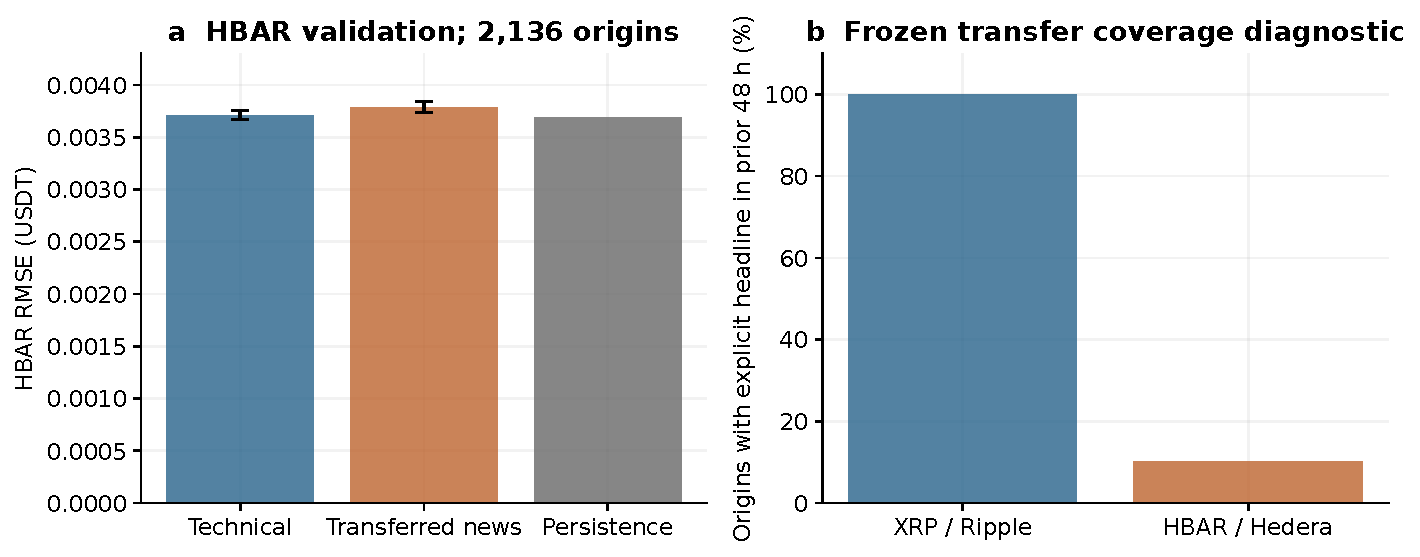
\includegraphics[width=.92\linewidth]{figures/fig15_hbar_transfer.pdf}
\caption{HBAR validation transfer results and asset-specific news coverage. The forecasting comparison is within HBAR; the coverage panel reports the share of validation origins with an explicit asset-name headline in the preceding 48 hours. Sparse coverage is a limitation, not an identified cause of the forecasting difference.}
\label{fig:hbar-transfer}
\end{figure}

% ============================================================
% SECTION 6: DISCUSSION AND LIMITATIONS
% ============================================================

\FloatBarrier
\section{Discussion and Limitations}
\label{sec:discussion}

\subsection{Incremental Predictive Value of News}
\label{subsec:discussion-news-value}

The central objective was to determine whether GPT-4o-derived news information provides incremental forecasting value beyond historical market data, technical indicators and BTC market context. The matched experiments provide a conditional answer. Both compact direct news and the best-performing sentiment-decay configuration achieved numerical improvements in validation RMSE relative to the technical-only BiLSTM. E1B achieved the largest improvement, reducing mean RMSE by 1.406\%, but this advantage was not statistically robust after the predefined multiple-comparison adjustment. The six-hour decay configuration achieved a smaller improvement of 0.466\%, and its adjusted uncertainty interval also included zero.

The later reserved retrospective evaluation assessed whether the selected validation advantage persisted. E1B produced 5.358\% higher arithmetic mean-seed RMSE than E0, while persistence achieved the lowest error. The tested news representations therefore did not establish a sustained forecasting advantage across the evaluated periods. This distinction matters because model selection and later-period evaluation answer different questions: a favourable validation result identifies a candidate, but it does not independently establish effectiveness under changing market conditions.

\subsection{Interpretation of the Sentiment-Decay Model}
\label{subsec:discussion-decay}

The sentiment-decay formulation provides an explicit mechanism for incorporating relevance and recency through specificity weighting and exponential temporal decay. The six-hour half-life achieved the strongest validation result within the tested grid. However, this mechanism is a feature-representation strategy, not a calibrated estimate of the causal market impact of an individual news event. Its transparency does not by itself establish predictive validity.

A supplementary evaluation of the frozen six-hour configuration also performed worse than E0 during the later retrospective period, with RMSE 1.426\% higher than the technical-only model. Because this check followed examination of the selected E1B results, it remains exploratory and cannot replace the original validation-selected model as the primary comparison. Taken together, the findings support treating the decay equation as a transparent experimental representation while leaving its generalisable predictive advantage unestablished.

\subsection{Temporal Alignment and Information Availability}
\label{subsec:discussion-timing}

The relationship between news publication and market movement is critical to cryptocurrency forecasting. Historical archives generally provide recorded publication timestamps, which may differ from the earliest public availability of the underlying information. An article describing a significant event may therefore appear after prices have already adjusted. Tariff announcements, regulatory developments and other XRP-related episodes illustrate the need to distinguish the underlying event, the archived publication and the observed market response.

For a forecast generated at time $t$, only information available at or before $t$ can legitimately contribute to the prediction; later publications must not enter its historical input sequence. Even when an article is correctly aligned to its recorded timestamp, its information may already be reflected in market prices. The forecasting task is therefore to determine whether the available features add information about the subsequent 24-hour movement, rather than merely recognise an important historical event.

The delayed-input sensitivity experiments did not reverse the retrospective E1B--E0 ranking. These tests do not establish that publication latency caused the observed deterioration. A causal explanation would require independently verified first-availability timestamps and a specifically designed latency intervention.

\subsection{Model Interpretability and Predictive Utility}
\label{subsec:discussion-interpretability}

Expected integrated gradients provides complementary evidence about the fitted model. Across the verified calculations, technical and market features accounted for 76.89\% of mean absolute attribution and news-related features for 23.11\%. The saved networks therefore respond to news-related inputs rather than ignoring them. These shares measure contributions within the trained forecasting function; they do not measure the causal contribution of news to prices or its incremental contribution to forecast accuracy.

The shares depend on the explained output, reference distribution, aggregation procedure and checkpoint. The verification retained the numerical completeness exceptions and documented variation across seeds and reference sets. Accordingly, the attribution and forecasting results are consistent: a model may use additional information without predicting more accurately than its technical-only control. Distinguishing \emph{feature utilisation} from \emph{predictive utility} is a central methodological finding of this study.

\subsection{Generalisation and Experimental Boundaries}
\label{subsec:discussion-generalisation}

Differences between validation and later-period performance may reflect changing market conditions, noisy annotations, overlap between technical and textual information, or sensitivity to model initialisation. The experiments establish the reversal in forecasting performance, the larger E1B seed variability and the absence of a statistically robust adjusted validation advantage. They do not identify which mechanism caused the deterioration.

Several design limitations define the scope of that conclusion. First, the archive provides retrospective publication timestamps rather than complete independently verified first-seen records, and empty intervals may indicate incomplete collection. Second, headline annotations do not capture all article content or related communications. GPT-4o scores are model-generated assessments rather than observed economic impacts. The 300-article provenance check concerns consistency of archived scoring records; it does not replace independent human assessment of annotation accuracy or inter-annotator agreement.

Third, validation was reused across experimental stages, creating potential selection optimism beyond within-stage multiplicity adjustments. The later period was reserved for the frozen comparison, but the wider historical archive had been examined during preceding research. Fourth, five seeds quantify training variability on the observed calendar rather than robustness across independent market regimes. Adding news also slightly changes the parameter count, although E0 and E1B retain the same architecture design and training procedure.

Finally, the supporting technical-only architecture comparisons use a different fitting target from the matched news experiments. They provide architectural context but cannot be pooled to estimate sentiment's incremental effect. Keeping these comparisons separate preserves their interpretation and the boundaries of the reported evidence.

\subsection{Practical Implications}
\label{subsec:discussion-implications}

A practical news-enhanced forecasting system requires more than improvement on a historical validation set. It should retain technical-only and persistence benchmarks, record first-observed news availability, monitor source coverage and annotation distributions, and evaluate paired errors across successive periods. Such monitoring can identify when a news-enhanced configuration ceases to add predictive value.

This study evaluates statistical forecasting performance rather than investment profitability. Transaction costs, spreads, execution delays and risk-adjusted trading outcomes were not evaluated. The reported metrics therefore do not establish profitable trading performance.

% ============================================================
% SECTION 7: FUTURE WORK
% ============================================================

\section{Future Work}
\label{sec:future-work}

For practical deployment, future studies should also assess forecasting stability, economic utility and trading costs. These extensions would help determine the conditions under which generative-AI-derived news information provides reliable incremental predictive value.

\section{Conclusion}
\label{sec:Conclusion}

This research investigated whether generative-AI-derived news information can enhance technical cryptocurrency price forecasting within a controlled bidirectional LSTM framework. The proposed approach combined historical XRP/USDT market observations, technical indicators, BTC market context and structured GPT-4o news features. The experimental protocol employed 30-hour historical input sequences, an exact 24-hour prediction horizon, chronological data partitions, training-only scaling and five-seed evaluation. 

The principal matched experiments demonstrated that compact direct-news features achieved the lowest validation RMSE among the evaluated configurations, with a numerical improvement of 1.406\% relative to technical-only BiLSTM. The proposed relevance-weighted sentiment-decay formulation provided a transparent alternative representation, with the six-hour half-life achieving the strongest result within its tested parameter grid. However, neither the direct-news advantage nor the decay-model improvement was established as statistically robust under the reported adjusted validation analysis. 

The reserved retrospective evaluation further demonstrated that the validation-selected news-enhanced model did not maintain its advantage. Its mean-seed RMSE was 5.358\% higher than the technical-only configuration, while persistence achieved the lowest error. 

The refined expected-integrated-gradients analysis attributed 76.89\% of mean absolute model sensitivity to technical and market inputs and 23.11\% to news-related features. These results confirm that the trained network incorporated the additional news information, while demonstrating that feature utilisation does not necessarily translate into improved forecasting performance. 

The separate HBAR transfer experiment also failed to establish an incremental benefit from the XRP-selected news representation. Its substantially lower asset-specific news coverage provides useful context, although coverage alone was not established as the cause of the observed result. 

The principal contribution of this study is a systematic and auditable evaluation of generative-AI-derived news features within a technical cryptocurrency forecasting framework. By distinguishing validation performance, statistical reliability, later-period generalisation, temporal information availability and model interpretability, the research provides evidence about both the potential and the boundaries of news-enhanced forecasting. The findings establish that successful integration of structured news information into a forecasting network does not, by itself, guarantee sustained predictive improvement.

\section*{Declarations}
\begingroup\small

\noindent\textbf{Funding and competing interests.}
No external funding or competing interests
were reported.

\par\noindent\textbf{Data and code availability.}
The prepared numerical model datasets, source code, frozen configurations, chronological split definitions, saved checkpoints, per-seed predictions, training histories, numerical verification outputs and figures are publicly available at \ResearchRepository. The repository is organised into named experimental subprojects and includes instructions for reproducing metrics from saved outputs. Redistribution of original news text remains subject to source-provider terms; the public release supplies the derived numerical model inputs and documents the remaining provenance and full-training reproducibility limitations.

\par\noindent\textbf{Ethics and annotation validation.}
The study uses historical market
observations and archived news headlines.
Independent human annotation validation
remains pending; consequently, no
human-derived accuracy or agreement
statistics are reported.

\par\noindent\textbf{Generative AI disclosure.}
GPT-derived headline annotations
constitute part of the research
methodology. 

% IMPORTANT:
% Preserve the COMPLETE existing bibliography below.
% Do not replace it with a shortened reference list.
% Preserve the existing \end{document} command.

\endgroup

\clearpage
\appendix
\section{Additional reproducibility results}\label{app:additional}
Tables~\ref{tab:epochs}--\ref{tab:shares} preserve selected epochs, every final-evaluation seed and every attribution pass. The technical controls retain their own target definition and selected epochs.

\begin{table}[!htbp]\centering\small
\caption{Selected validation epochs for seeds in fixed order.}\label{tab:epochs}
\begin{tabular}{lrrrrrl}\toprule
Model & 42 & 123 & 2026 & 7 & 99 & Parameters\\\midrule
Technical BiLSTM & 3 & 2 & 3 & 1 & 2 & 564353 \\
Direct news hybrid & 6 & 4 & 2 & 3 & 2 & 570497 \\
Decay 3 h & 3 & 4 & 3 & 1 & 2 & 566401 \\
Decay 6 h & 3 & 1 & 1 & 3 & 2 & 566401 \\
Decay 12 h & 3 & 1 & 1 & 1 & 2 & 566401 \\
Decay 24 h & 1 & 1 & 1 & 4 & 2 & 566401 \\

\bottomrule\end{tabular}
\tabnote{All parameters are trainable. Selection is by minimum validation scaled-return MSE.}
\end{table}


\begin{table}[!htbp]\centering\small
\caption{Selected epochs for the absolute-price technical controls.}\label{tab:benchepochs}
\begin{tabular}{lrrrrrl}\toprule
Model & 42 & 123 & 2026 & 7 & 99 & Parameters\\\midrule
BiLSTM with BTC & 1 & 2 & 2 & 1 & 1 & 564353 \\
BiLSTM without BTC & 2 & 12 & 2 & 11 & 6 & 563329 \\
LSTM 128 with BTC & 1 & 2 & 1 & 9 & 13 & 216705 \\
LSTM 210 with BTC & 1 & 7 & 2 & 3 & 2 & 562089 \\

\bottomrule\end{tabular}
\tabnote{The same five seeds are retained for every recurrent control. ARIMAX has no neural epoch. These epochs do not refer to the return-trained E0.}
\end{table}

\begin{table}[!htbp]\centering\small
\caption{Individual later-period results; no favourable seed is omitted.}\label{tab:seeds}
\begin{tabular}{lrrrrrr}\toprule
Model & Seed & Epoch & RMSE & MAE & $R^2$ & DA \%\\\midrule
E0 & 42 & 3 & 0.040061 & 0.027502 & 0.934918 & 45.86 \\
E0 & 123 & 2 & 0.039976 & 0.027606 & 0.935193 & 48.65 \\
E0 & 2026 & 3 & 0.040330 & 0.027665 & 0.934041 & 53.06 \\
E0 & 7 & 1 & 0.039732 & 0.027383 & 0.935981 & 49.49 \\
E0 & 99 & 2 & 0.039782 & 0.027006 & 0.935819 & 50.97 \\
E1B & 42 & 6 & 0.049553 & 0.031123 & 0.900422 & 48.57 \\
E1B & 123 & 4 & 0.040979 & 0.027888 & 0.931900 & 45.32 \\
E1B & 2026 & 2 & 0.040121 & 0.027353 & 0.934722 & 53.04 \\
E1B & 7 & 3 & 0.039586 & 0.027515 & 0.936450 & 47.91 \\
E1B & 99 & 2 & 0.040350 & 0.027692 & 0.933974 & 52.34 \\
\bottomrule\end{tabular}
\end{table}

\begin{table}[!htbp]\centering\small
\caption{All attribution passes for the E1B model.}\label{tab:shares}
\begin{tabular}{rrrrr}\toprule
Seed & Reference & Technical \% & News \% & Tolerance failures\\\midrule
42 & 0 & 75.66 & 24.34 & 0 \\
42 & 1 & 79.06 & 20.94 & 52 \\
123 & 0 & 80.11 & 19.89 & 0 \\
123 & 1 & 81.55 & 18.45 & 0 \\
2026 & 0 & 77.82 & 22.18 & 0 \\
2026 & 1 & 74.67 & 25.33 & 0 \\
7 & 0 & 79.63 & 20.37 & 0 \\
7 & 1 & 79.54 & 20.46 & 0 \\
99 & 0 & 72.16 & 27.84 & 0 \\
99 & 1 & 68.68 & 31.32 & 0 \\
\bottomrule\end{tabular}
\tabnote{Each pass contains 1,000 explanations. Reference sets contain 32 training sequences. The technical/news split is based on absolute expected integrated-gradient contributions to unscaled predicted log return, not exact SHAP or causal market effects.}
\end{table}


\begin{table}[htbp]\centering\small
\caption{All primary validation seeds; metrics use reconstructed price.}\label{tab:validationseeds}
\begin{tabular}{lrrrrr}\toprule
Model & Seed & RMSE & MAE & $R^2$ & DA \%\\\midrule
E0 & 42 & 0.064064 & 0.045029 & 0.951765 & 48.74\\
E0 & 123 & 0.063668 & 0.044608 & 0.952359 & 54.82\\
E0 & 2026 & 0.063917 & 0.044337 & 0.951986 & 56.79\\
E0 & 7 & 0.064558 & 0.044965 & 0.951018 & 51.31\\
E0 & 99 & 0.063469 & 0.043630 & 0.952657 & 57.26\\
E1B & 42 & 0.062431 & 0.043774 & 0.954192 & 56.98\\
E1B & 123 & 0.062889 & 0.043997 & 0.953518 & 53.75\\
E1B & 2026 & 0.063212 & 0.043576 & 0.953039 & 58.05\\
E1B & 7 & 0.063260 & 0.044458 & 0.952968 & 53.51\\
E1B & 99 & 0.063389 & 0.044139 & 0.952776 & 57.07\\
E2\_h3 & 42 & 0.063613 & 0.044502 & 0.952441 & 54.31\\
E2\_h3 & 123 & 0.063288 & 0.043818 & 0.952926 & 56.60\\
E2\_h3 & 2026 & 0.063898 & 0.044517 & 0.952015 & 48.13\\
E2\_h3 & 7 & 0.064758 & 0.045660 & 0.950713 & 46.63\\
E2\_h3 & 99 & 0.063062 & 0.043667 & 0.953262 & 55.71\\
E2\_h6 & 42 & 0.063055 & 0.043938 & 0.953272 & 53.93\\
E2\_h6 & 123 & 0.063192 & 0.044050 & 0.953068 & 56.41\\
E2\_h6 & 2026 & 0.063811 & 0.044680 & 0.952145 & 54.54\\
E2\_h6 & 7 & 0.064909 & 0.046749 & 0.950484 & 48.69\\
E2\_h6 & 99 & 0.063217 & 0.043637 & 0.953031 & 56.65\\
E2\_h12 & 42 & 0.063187 & 0.043936 & 0.953077 & 58.43\\
E2\_h12 & 123 & 0.063170 & 0.044121 & 0.953102 & 55.01\\
E2\_h12 & 2026 & 0.064203 & 0.044943 & 0.951554 & 53.79\\
E2\_h12 & 7 & 0.066240 & 0.047651 & 0.948433 & 45.46\\
E2\_h12 & 99 & 0.063295 & 0.043547 & 0.952916 & 55.99\\
E2\_h24 & 42 & 0.065146 & 0.045507 & 0.950122 & 48.46\\
E2\_h24 & 123 & 0.063261 & 0.044263 & 0.952967 & 54.82\\
E2\_h24 & 2026 & 0.064245 & 0.044876 & 0.951492 & 52.90\\
E2\_h24 & 7 & 0.065537 & 0.046425 & 0.949521 & 43.87\\
E2\_h24 & 99 & 0.063516 & 0.043802 & 0.952586 & 53.56\\\bottomrule\end{tabular}
\tabnote{Seeds describe optimisation variation in the same market period, not five independent temporal replications.}
\end{table}

\begin{table}[htbp]\centering\small
\caption{Supplementary later E2 six-hour results from frozen checkpoints.}\label{tab:e2laterseeds}
\begin{tabular}{rrrrr}\toprule
Seed & RMSE & MAE & $R^2$ & DA \%\\\midrule
42 & 0.040305 & 0.027563 & 0.934120 & 49.22\\
123 & 0.040160 & 0.027514 & 0.934593 & 47.34\\
2026 & 0.040104 & 0.027834 & 0.934778 & 50.38\\
7 & 0.042269 & 0.029181 & 0.927544 & 48.76\\
99 & 0.039891 & 0.027111 & 0.935467 & 51.86\\\bottomrule\end{tabular}
\tabnote{Post-exposure analysis without retraining or replacement of the validation-selected E1B model.}
\end{table}

\begin{table}[htbp]\centering\small
\caption{Exploratory conditional risks: validation period.}\label{tab:conditionalall}
\begin{tabular}{p{.30\linewidth}rrrrp{.22\linewidth}}\toprule
Condition & $n$ & E0 & E1B & Change \% & Adjusted interval\\\midrule
High volatility & 107 & 0.091356 & 0.086339 & -5.49 & [-0.00873,0.00107]\\
Other volatility & 2029 & 0.062155 & 0.061564 & -0.95 & [-0.00185,0.00043]\\
Current-hour news & 903 & 0.066480 & 0.065664 & -1.23 & [-0.00223,0.00064]\\
No current-hour news & 1233 & 0.062007 & 0.061041 & -1.56 & [-0.00256,0.00035]\\
XRP-specific news within 6h & 1995 & 0.062607 & 0.061942 & -1.06 & [-0.00179,0.00039]\\
No XRP-specific news within 6h & 141 & 0.080424 & 0.076878 & -4.41 & [-0.00817,0.00291]\\
Positive XRP stance & 446 & 0.066105 & 0.065067 & -1.57 & [-0.00269,0.00049]\\
Negative XRP stance & 124 & 0.055649 & 0.054439 & -2.17 & [-0.00275,0.00064]\\
High specificity with news & 784 & 0.067635 & 0.066673 & -1.42 & [-0.00244,0.00058]\\
Lower specificity with news & 119 & 0.058303 & 0.058590 & +0.49 & [-0.00112,0.00176]\\
High uncertainty with news & 490 & 0.066844 & 0.066107 & -1.10 & [-0.00217,0.00071]\\
Lower uncertainty with news & 413 & 0.066046 & 0.065136 & -1.38 & [-0.00249,0.00078]\\
High trailing24h article count & 254 & 0.096113 & 0.094259 & -1.93 & [-0.00548,0.00208]\\
Other trailing24h article count & 1882 & 0.058248 & 0.057540 & -1.21 & [-0.00205,0.00042]\\
Curated event window & 24 & 0.040513 & 0.041725 & +2.99 & Not estimable\\
Outside curated event window & 2112 & 0.064153 & 0.063238 & -1.43 & [-0.00219,0.00034]\\\bottomrule\end{tabular}
\tabnote{RMSE is square-root mean-seed risk, not arithmetic mean seed RMSE. Negative change favours news. Intervals are 99.84375\% calendar-block intervals over 32 contrasts; 50,000 resamples; endpoint Monte Carlo brackets and block sensitivity are supplied separately; small strata remain imprecise. No subgroup has an adjusted improvement.}
\end{table}

\begin{table}[htbp]\centering\small
\caption{Exploratory conditional risks: later period.}\label{tab:conditionallater}
\begin{tabular}{p{.30\linewidth}rrrrp{.22\linewidth}}\toprule
Condition & $n$ & E0 & E1B & Change \% & Adjusted interval\\\midrule
High volatility & 152 & 0.103221 & 0.114542 & +10.97 & [-0.00144,0.03298]\\
Other volatility & 5110 & 0.036452 & 0.038090 & +4.49 & [-0.00007,0.00525]\\
Current-hour news & 1633 & 0.037802 & 0.039145 & +3.55 & [-0.00020,0.00353]\\
No current-hour news & 3629 & 0.040917 & 0.043623 & +6.61 & [0.00014,0.00668]\\
XRP-specific news within 6h & 4276 & 0.038867 & 0.041113 & +5.78 & [-0.00000,0.00579]\\
No XRP-specific news within 6h & 986 & 0.044471 & 0.047025 & +5.74 & [0.00006,0.00602]\\
Positive XRP stance & 723 & 0.039908 & 0.041553 & +4.12 & [-0.00031,0.00434]\\
Negative XRP stance & 205 & 0.033446 & 0.033596 & +0.45 & [-0.00133,0.00229]\\
High specificity with news & 1263 & 0.037850 & 0.039471 & +4.28 & [-0.00009,0.00402]\\
Lower specificity with news & 370 & 0.037640 & 0.038010 & +0.98 & [-0.00108,0.00258]\\
High uncertainty with news & 904 & 0.035198 & 0.035910 & +2.02 & [-0.00056,0.00288]\\
Lower uncertainty with news & 729 & 0.040802 & 0.042818 & +4.94 & [-0.00008,0.00499]\\
High trailing24h article count & 579 & 0.034095 & 0.033627 & -1.37 & [-0.00169,0.00113]\\
Other trailing24h article count & 4683 & 0.040645 & 0.043234 & +6.37 & [0.00016,0.00617]\\
Curated event window & 48 & 0.139955 & 0.144324 & +3.12 & Not estimable\\
Outside curated event window & 5214 & 0.037849 & 0.040158 & +6.10 & [0.00006,0.00575]\\\bottomrule\end{tabular}
\tabnote{RMSE is square-root mean-seed risk, not arithmetic mean seed RMSE. Negative change favours news. Intervals are 99.84375\% calendar-block intervals over 32 contrasts; 50,000 resamples; endpoint Monte Carlo brackets and block sensitivity are supplied separately; small strata remain imprecise. No subgroup has an adjusted improvement.}
\end{table}

\begin{figure}[htbp]\centering
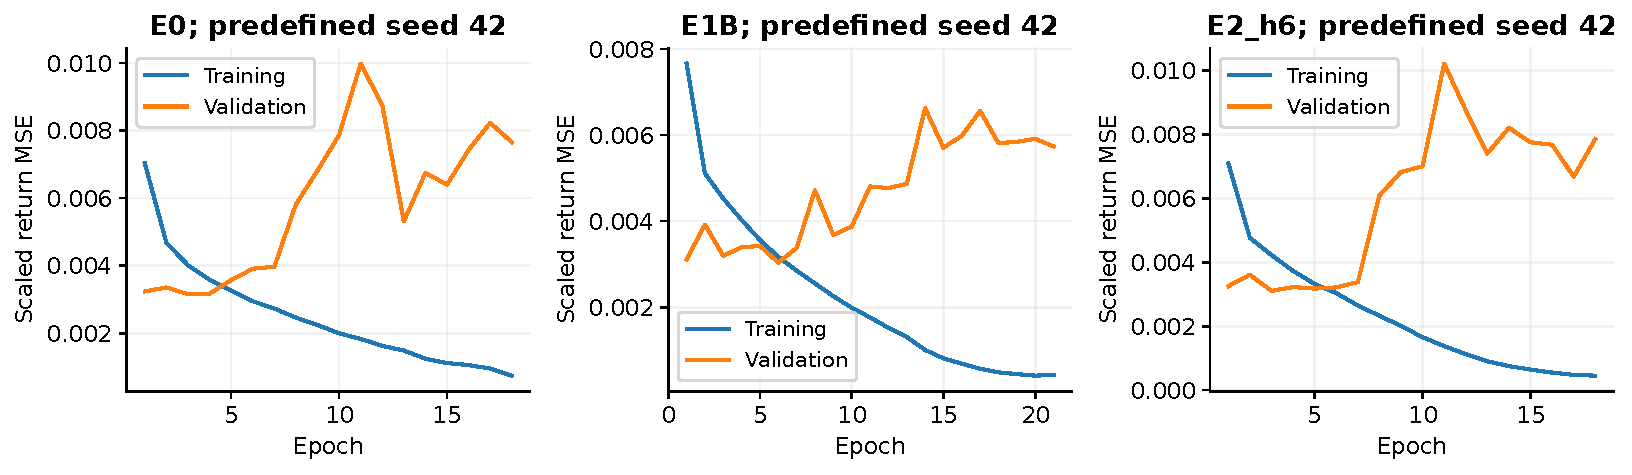
\includegraphics[width=.98\linewidth]{figures/figS01_training_diagnostics.pdf}
\caption{Saved training and validation scaled-return MSE for seed 42, selected in advance as the representative plotting rule. All other histories and selected epochs remain available. Early selected epochs are not overwritten by increasing training.}\label{fig:training}
\end{figure}

\begin{figure}[htbp]\centering
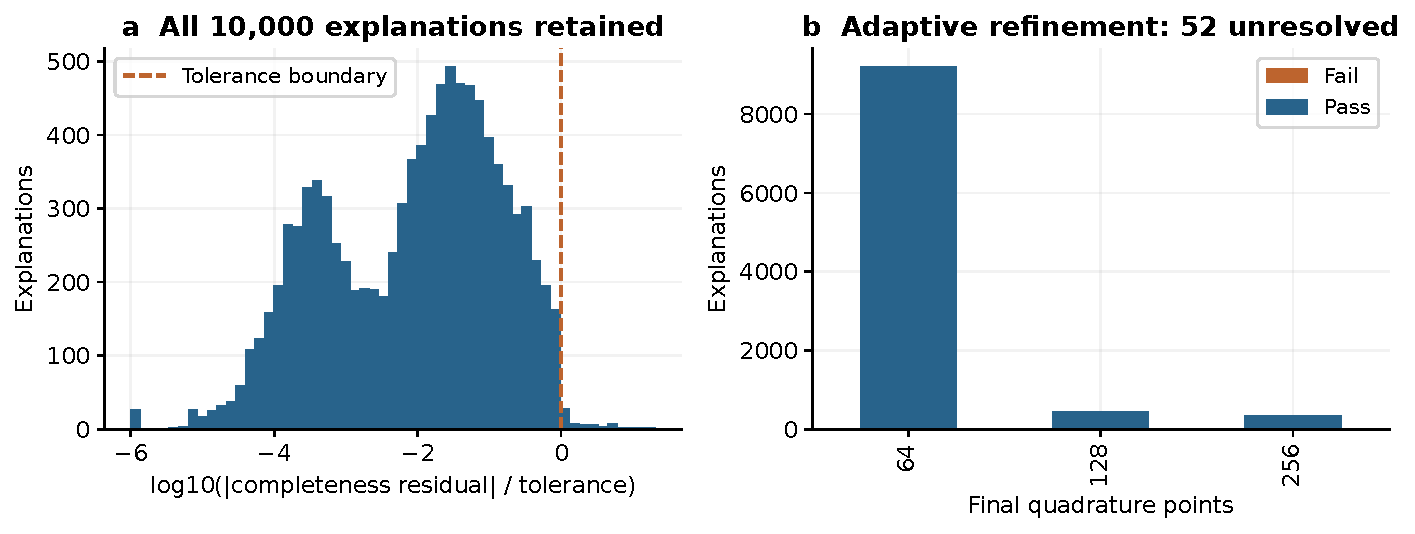
\includegraphics[width=.98\linewidth]{figures/figS02_precision_diagnostics.pdf}
\caption{Completeness residual-to-tolerance ratios and adaptive quadrature counts. All 10,000 explanations remain in the primary shares; 52 fail tolerance. A small total residual cannot guarantee featurewise convergence.}\label{fig:precision}
\end{figure}

\FloatBarrier
\begin{thebibliography}{99}
\bibitem[Alessandretti et~al.(2018)]{Alessandretti2018} Alessandretti, L., ElBahrawy, A., Aiello, L.M., Baronchelli, A., 2018. Anticipating cryptocurrency prices using machine learning. Complexity 2018, 8983590. \doi{10.1155/2018/8983590}.
\bibitem[American Presidency Project(2025a)]{APP2025April} American Presidency Project, 2025a. Truth Social posts of April 9, 2025. Presidential post archive; displayed times Pacific. \url{https://www.presidency.ucsb.edu/documents/truth-social-posts-april-9-2025}.
\bibitem[American Presidency Project(2025b)]{APP2025October} American Presidency Project, 2025b. Truth Social posts of October 10, 2025. Presidential post archive; displayed times Pacific. \url{https://www.presidency.ucsb.edu/documents/truth-social-posts-october-10-2025}.
\bibitem[Araci(2019)]{Araci2019} Araci, D., 2019. FinBERT: Financial sentiment analysis with pre-trained language models. MSc thesis preprint, arXiv:1908.10063. \url{https://arxiv.org/abs/1908.10063}.
\bibitem[Baltrusaitis et~al.(2019)]{Baltrusaitis2019} Baltru\v{s}aitis, T., Ahuja, C., Morency, L.-P., 2019. Multimodal machine learning: A survey and taxonomy. IEEE Transactions on Pattern Analysis and Machine Intelligence 41, 423--443. \doi{10.1109/TPAMI.2018.2798607}.
\bibitem[Bergmeir et~al.(2018)]{Bergmeir2018} Bergmeir, C., Hyndman, R.J., Koo, B., 2018. A note on the validity of cross-validation for evaluating autoregressive time series prediction. Computational Statistics \& Data Analysis 120, 70--83. \doi{10.1016/j.csda.2017.11.003}.
\bibitem[Bollen et~al.(2011)]{Bollen2011} Bollen, J., Mao, H., Zeng, X., 2011. Twitter mood predicts the stock market. Journal of Computational Science 2, 1--8. \doi{10.1016/j.jocs.2010.12.007}.
\bibitem[Erion et~al.(2021)]{Erion2021} Erion, G., Janizek, J.D., Sturmfels, P., Lundberg, S.M., Lee, S.-I., 2021. Improving performance of deep learning models with axiomatic attribution priors and expected gradients. Nature Machine Intelligence 3, 620--631. \doi{10.1038/s42256-021-00343-w}.
\bibitem[Fama(1970)]{Fama1970} Fama, E.F., 1970. Efficient capital markets: A review of theory and empirical work. Journal of Finance 25, 383--417. \doi{10.1111/j.1540-6261.1970.tb00518.x}.
\bibitem[Fischer and Krauss(2018)]{Fischer2018} Fischer, T., Krauss, C., 2018. Deep learning with long short-term memory networks for financial market predictions. European Journal of Operational Research 270, 654--669. \doi{10.1016/j.ejor.2017.11.054}.
\bibitem[Hochreiter and Schmidhuber(1997)]{Hochreiter1997} Hochreiter, S., Schmidhuber, J., 1997. Long short-term memory. Neural Computation 9, 1735--1780. \doi{10.1162/neco.1997.9.8.1735}.
\bibitem[Hyndman and Athanasopoulos(2021)]{Hyndman2021} Hyndman, R.J., Athanasopoulos, G., 2021. Forecasting: Principles and Practice, third ed. OTexts, Melbourne. \url{https://otexts.com/fpp3/}.
\bibitem[Kingma and Ba(2015)]{Kingma2015} Kingma, D.P., Ba, J., 2015. Adam: A method for stochastic optimization. International Conference on Learning Representations. \url{https://arxiv.org/abs/1412.6980}.
\bibitem[Kraaijeveld and De Smedt(2020)]{Kraaijeveld2020} Kraaijeveld, O., De Smedt, J., 2020. The predictive power of public Twitter sentiment for forecasting cryptocurrency prices. Journal of International Financial Markets, Institutions and Money 65, 101188. \doi{10.1016/j.intfin.2020.101188}.
\bibitem[Kunsch(1989)]{Kunsch1989} Kunsch, H.R., 1989. The jackknife and the bootstrap for general stationary observations. Annals of Statistics 17, 1217--1241. \doi{10.1214/aos/1176347265}.
\bibitem[Lopez-Lira and Tang(2023)]{LopezLira2023} Lopez-Lira, A., Tang, Y., 2023. Can ChatGPT forecast stock price movements? Return predictability and large language models. arXiv:2304.07619, revised 2025. \doi{10.48550/arXiv.2304.07619}.
\bibitem[Lundberg and Lee(2017)]{Lundberg2017} Lundberg, S.M., Lee, S.-I., 2017. A unified approach to interpreting model predictions. Advances in Neural Information Processing Systems 30. \url{https://arxiv.org/abs/1705.07874}.
\bibitem[Newey and West(1987)]{Newey1987} Newey, W.K., West, K.D., 1987. A simple, positive semi-definite, heteroskedasticity and autocorrelation consistent covariance matrix. Econometrica 55, 703--708. \doi{10.2307/1913610}.
\bibitem[Schuster and Paliwal(1997)]{Schuster1997} Schuster, M., Paliwal, K.K., 1997. Bidirectional recurrent neural networks. IEEE Transactions on Signal Processing 45, 2673--2681. \doi{10.1109/78.650093}.
\bibitem[Sezer et~al.(2020)]{Sezer2020} Sezer, O.B., Gudelek, M.U., Ozbayoglu, A.M., 2020. Financial time series forecasting with deep learning: A systematic literature review, 2005--2019. Applied Soft Computing 90, 106181. \doi{10.1016/j.asoc.2020.106181}.
\bibitem[statsmodels developers(2026)]{Statsmodels2026} statsmodels developers, 2026. SARIMAX: regression with seasonal ARIMA errors. Official documentation, accessed 8 November 2026. \url{https://www.statsmodels.org/stable/generated/statsmodels.tsa.statespace.sarimax.SARIMAX.html}.
\bibitem[Sullivan et~al.(1999)]{Sullivan1999} Sullivan, R., Timmermann, A., White, H., 1999. Data-snooping, technical trading rule performance, and the bootstrap. Journal of Finance 54, 1647--1691. \doi{10.1111/0022-1082.00163}.
\bibitem[Sundararajan et~al.(2017)]{Sundararajan2017} Sundararajan, M., Taly, A., Yan, Q., 2017. Axiomatic attribution for deep networks. Proceedings of Machine Learning Research 70, 3319--3328. \url{https://proceedings.mlr.press/v70/sundararajan17a.html}.
\bibitem[Tetlock(2007)]{Tetlock2007} Tetlock, P.C., 2007. Giving content to investor sentiment: The role of media in the stock market. Journal of Finance 62, 1139--1168. \doi{10.1111/j.1540-6261.2007.01232.x}.
\bibitem[U.S. Government Publishing Office(2025)]{GovInfo2025} U.S. Government Publishing Office, 2025. Remarks Announcing Additional United States Tariff Actions on Foreign Imports, 2 April 2025. Daily Compilation of Presidential Documents, DCPD-202500423. \url{https://www.govinfo.gov/content/pkg/DCPD-202500423/html/DCPD-202500423.htm}.
\bibitem[U.S. Securities and Exchange Commission(2026)]{SEC2026} U.S. Securities and Exchange Commission, 2026. SEC proposes new Regulation Crypto Assets. Press release 2026-76, 18 August. \url{https://www.sec.gov/newsroom/press-releases/2026-76-sec-proposes-new-regulation-crypto-assets}.
\bibitem[Bollerslev(1986)]{Bollerslev1986}
Bollerslev, T., 1986. Generalized autoregressive conditional heteroskedasticity. Journal of Econometrics 31(3), 307--327. \url{https://doi.org/10.1016/0304-4076(86)90063-1}.

\bibitem[Nelson(1991)]{Nelson1991}
Nelson, D.B., 1991. Conditional heteroskedasticity in asset returns: A new approach. Econometrica 59(2), 347--370. \url{https://doi.org/10.2307/2938260}.

\bibitem[Tay and Cao(2001)]{Tay2001}
Tay, F.E.H., Cao, L., 2001. Application of support vector machines in financial time series forecasting. Omega 29(4), 309--317. \url{https://doi.org/10.1016/S0305-0483(01)00026-3}.

\bibitem[Hamayel and Owda(2021)]{Hamayel2021}
Hamayel, M.J., Owda, A.Y., 2021. A novel cryptocurrency price prediction model using GRU, LSTM and bi-LSTM machine learning algorithms. AI 2(4), 477--496. \url{https://doi.org/10.3390/ai2040030}.

\bibitem[Young(2025)]{Young2025} Young, M., 2025. Bitcoin Price Plummets to \$82K in Reaction to Trump Tariffs. CryptoPotato, 3 April 2025, 05:41 UTC. \url{https://cryptopotato.com/bitcoin-price-plummets-to-82k-in-reaction-to-trump-tariffs/}.
\end{thebibliography}
\end{document}
